%\setcounter{chapter}{7}
\chapter{Module Production for the Phase I CMS Pixel Detector Upgrade}\label{ch:phase1}

As discussed in chapter \ref{ch:lhcandcms} the CMS pixel detector will \ital{suffer} from radiation damage throughout its lifetime hence the need for periodical updates. The first version of the detector was known as phase 0, it became fully operational 2010 after solving a setback during the original starting period in 2008. In 2017 the pixel detector was replaced during the so-called phase 1 upgrade, the University of Nebraska, high energy group (UNL-HEP) played a major role in assembling and testing over 500 modules, from 2013 to 2016, which then became part of the forward region of the pixel detector (FPix). The next update of this detector (phase 2) is projected to take place in 2025 when the current detector will be reaching its limits. In this chapter we describe why the phase 0 pixel detector needed an upgrade making 

the work done by the UNL-HEP group. Some of these steps will be highlighted and described in detail as they were my contributions to this production campaign. Specially the  and highlighting 

\section{The CMS Pixel Detector Phase I Upgrade}
The CMS pixel detector is composed of two sections, the barrel section (BPix) and the forward section (FPix). Each of these sections (for phase 0) was composed of three layers originally designed to record three 3D positions (tracks) of the particles emerging from the \ital{pp} collisions. As well as to provide information to reconstruct primary and secondary vertices of decaying particles. This detector performed well during the LHC run I,{\rojo{incorporate the bunch crossing?}} taking data at the design luminosity of $1 x 10^{34} cm^{-2} s^{-1}$, which was then used in many analysis including the discovery of the Higgs bosson published in 2013. But after a few years of operation the pixel detector started to degrade due to radiation damage, causing an increase of fake rates as well as loose on resolution. Moreover, for run II the LHC planned to double the luminosity with successive increment until reach its peak of $2 x 10^{35} cm^{-2} s^{-1}$. A simulation of the performance of the pixel detector under different luminosity conditions can be seen in figure \ref{fig:red_perf}

\begin{figure}[!h]
\centering
\includegraphics[width=0.9\textwidth]{ch7/reducedperformance}
%\includegraphics[width=0.9\textwidth]{pixel/reducedperformance}
\caption[Expected performance of the original pixel detector for different luminosities.]{Expected performance of the original pixel detector under different luminosity conditions: a) track-finding efficiency; b) fake rate. Conventions are the same for both plots, considering zero pileup (blue squares), average pileup of 25 (red dots), average pileup of 50 (black diamonds), and average pileup of 100 (magenta triangles).\cite{pix_tdr}}\label{fig:red_perf}
\end{figure}

This degradation prompted the need for an improved pixel detector. It was designed to have four layers in the barrel ubicated at distances of Hena2420
and 3 layers at each endcap as shown in \ref{fig:new_pix}. better

\begin{figure}[!h]
\centering
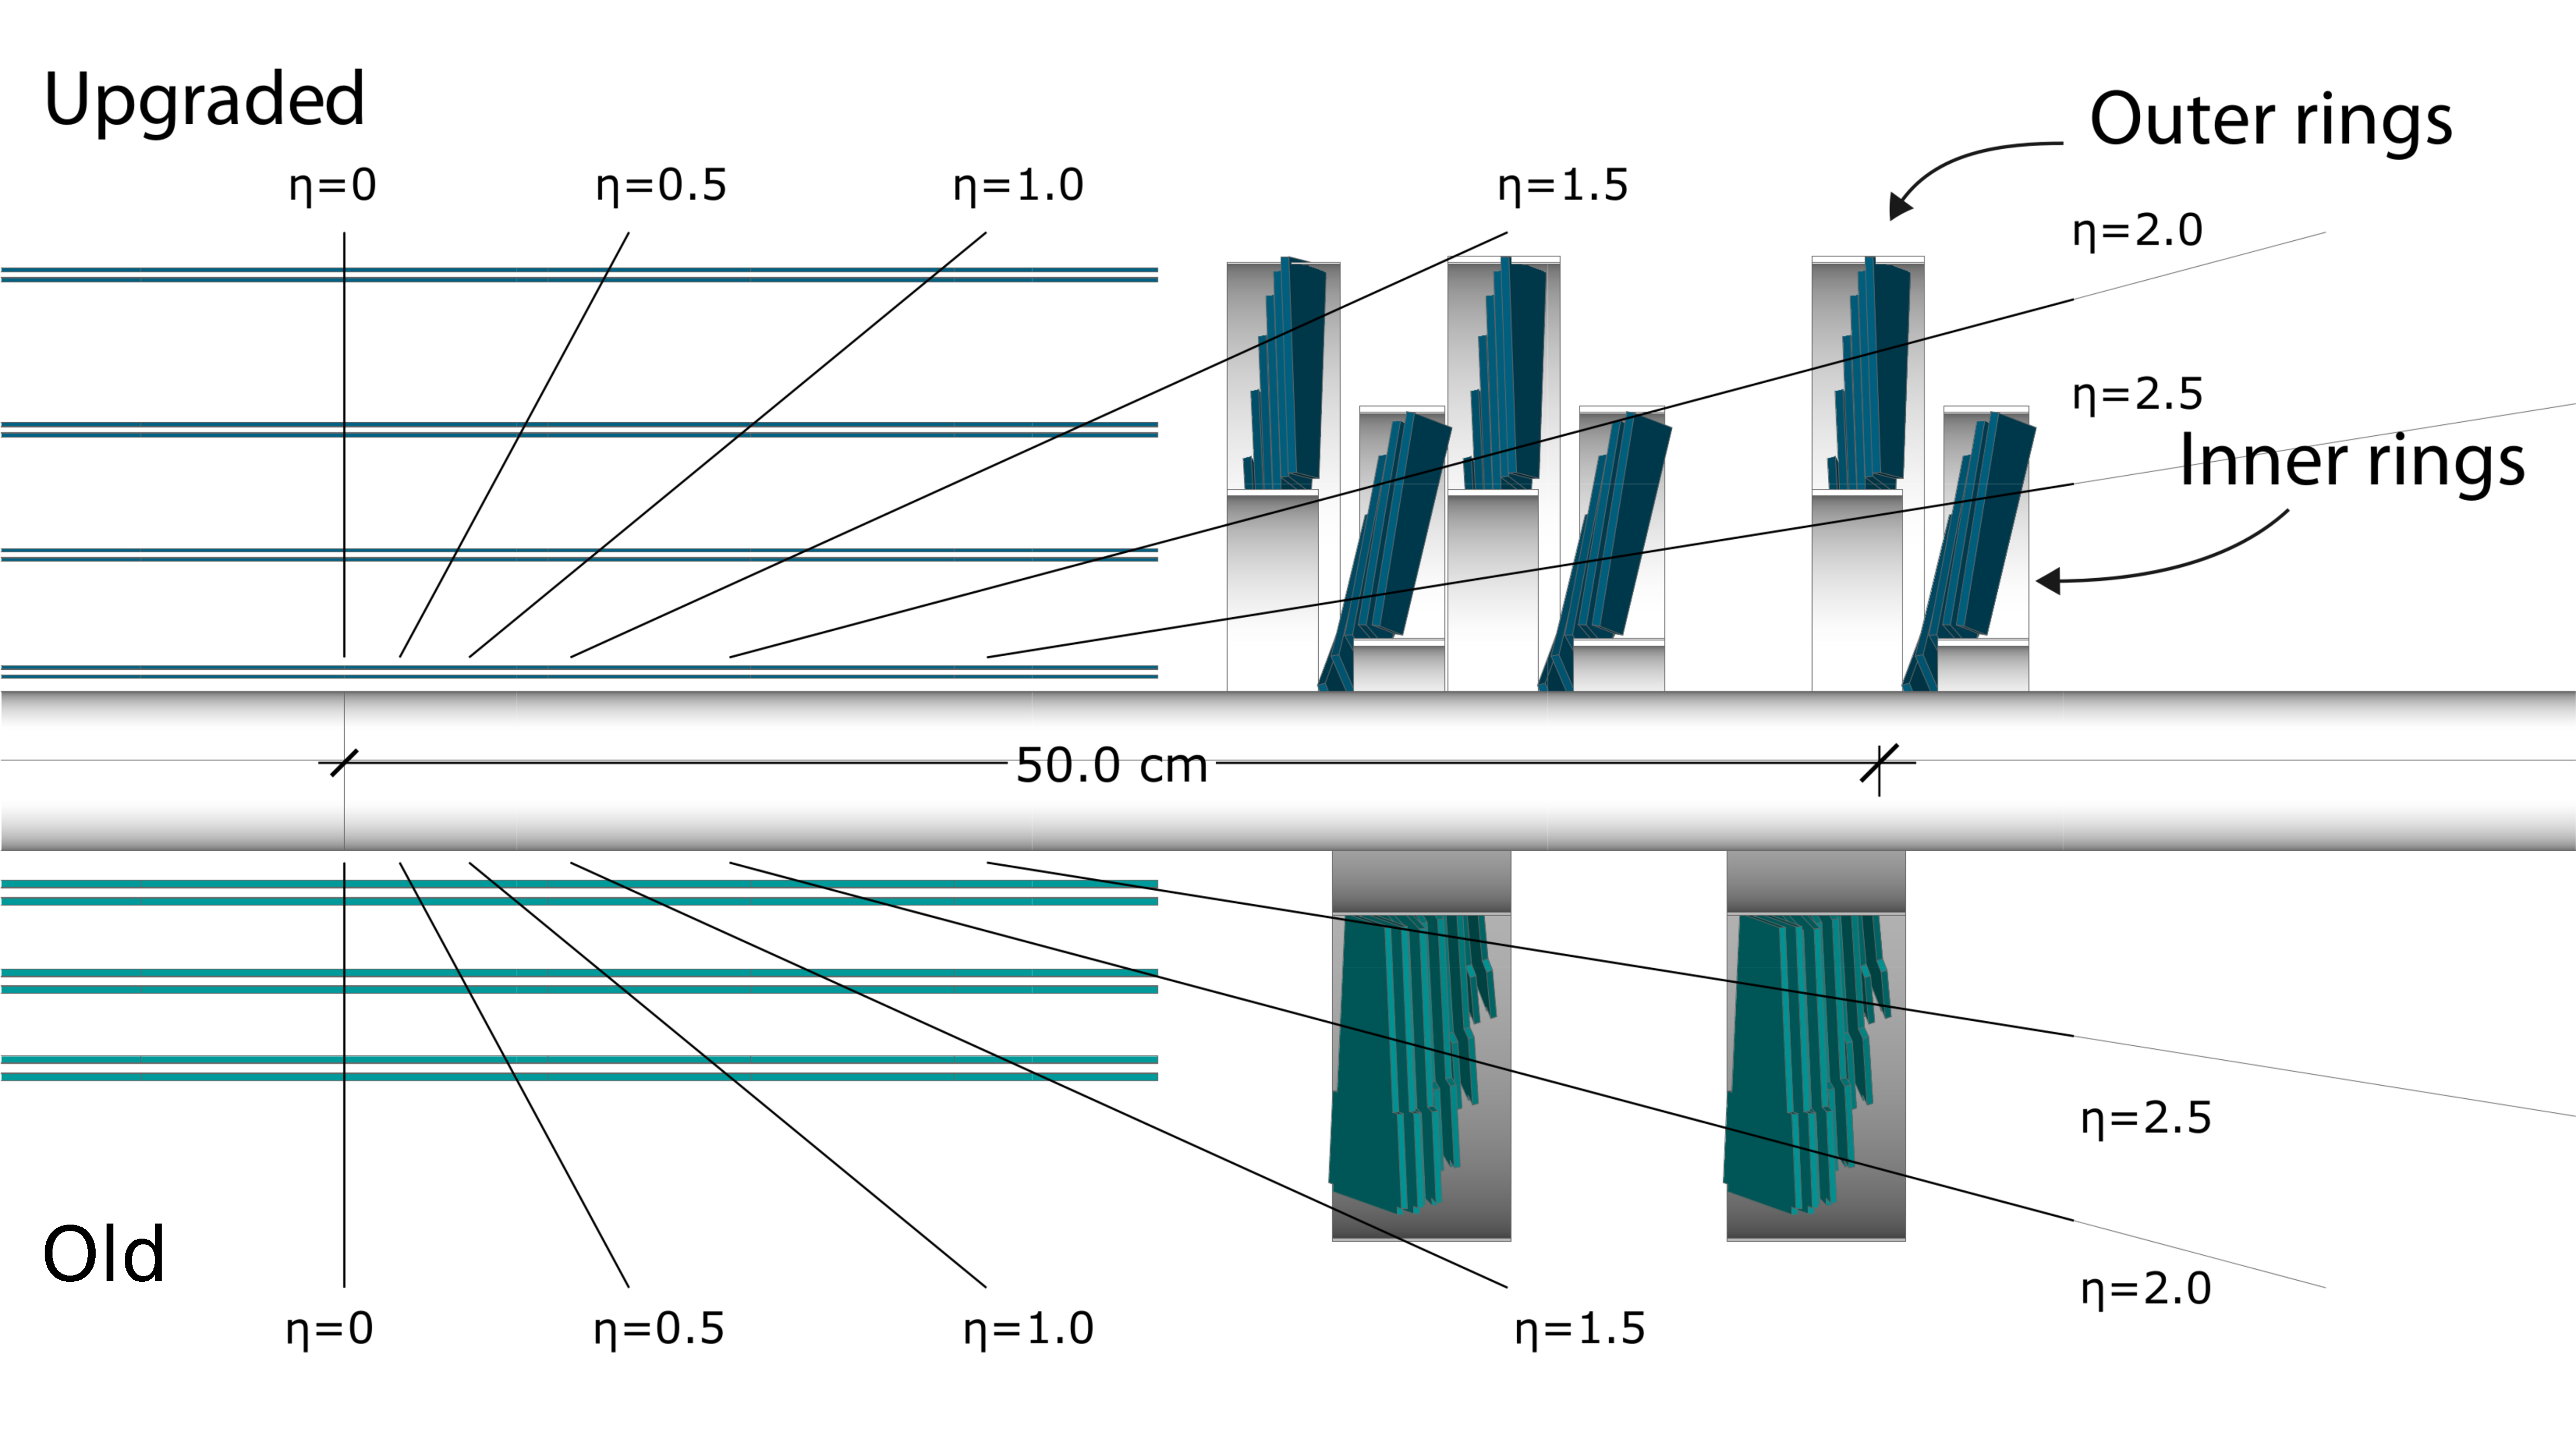
\includegraphics[width=0.6\textwidth]{../images/ch7/fpix.pdf}
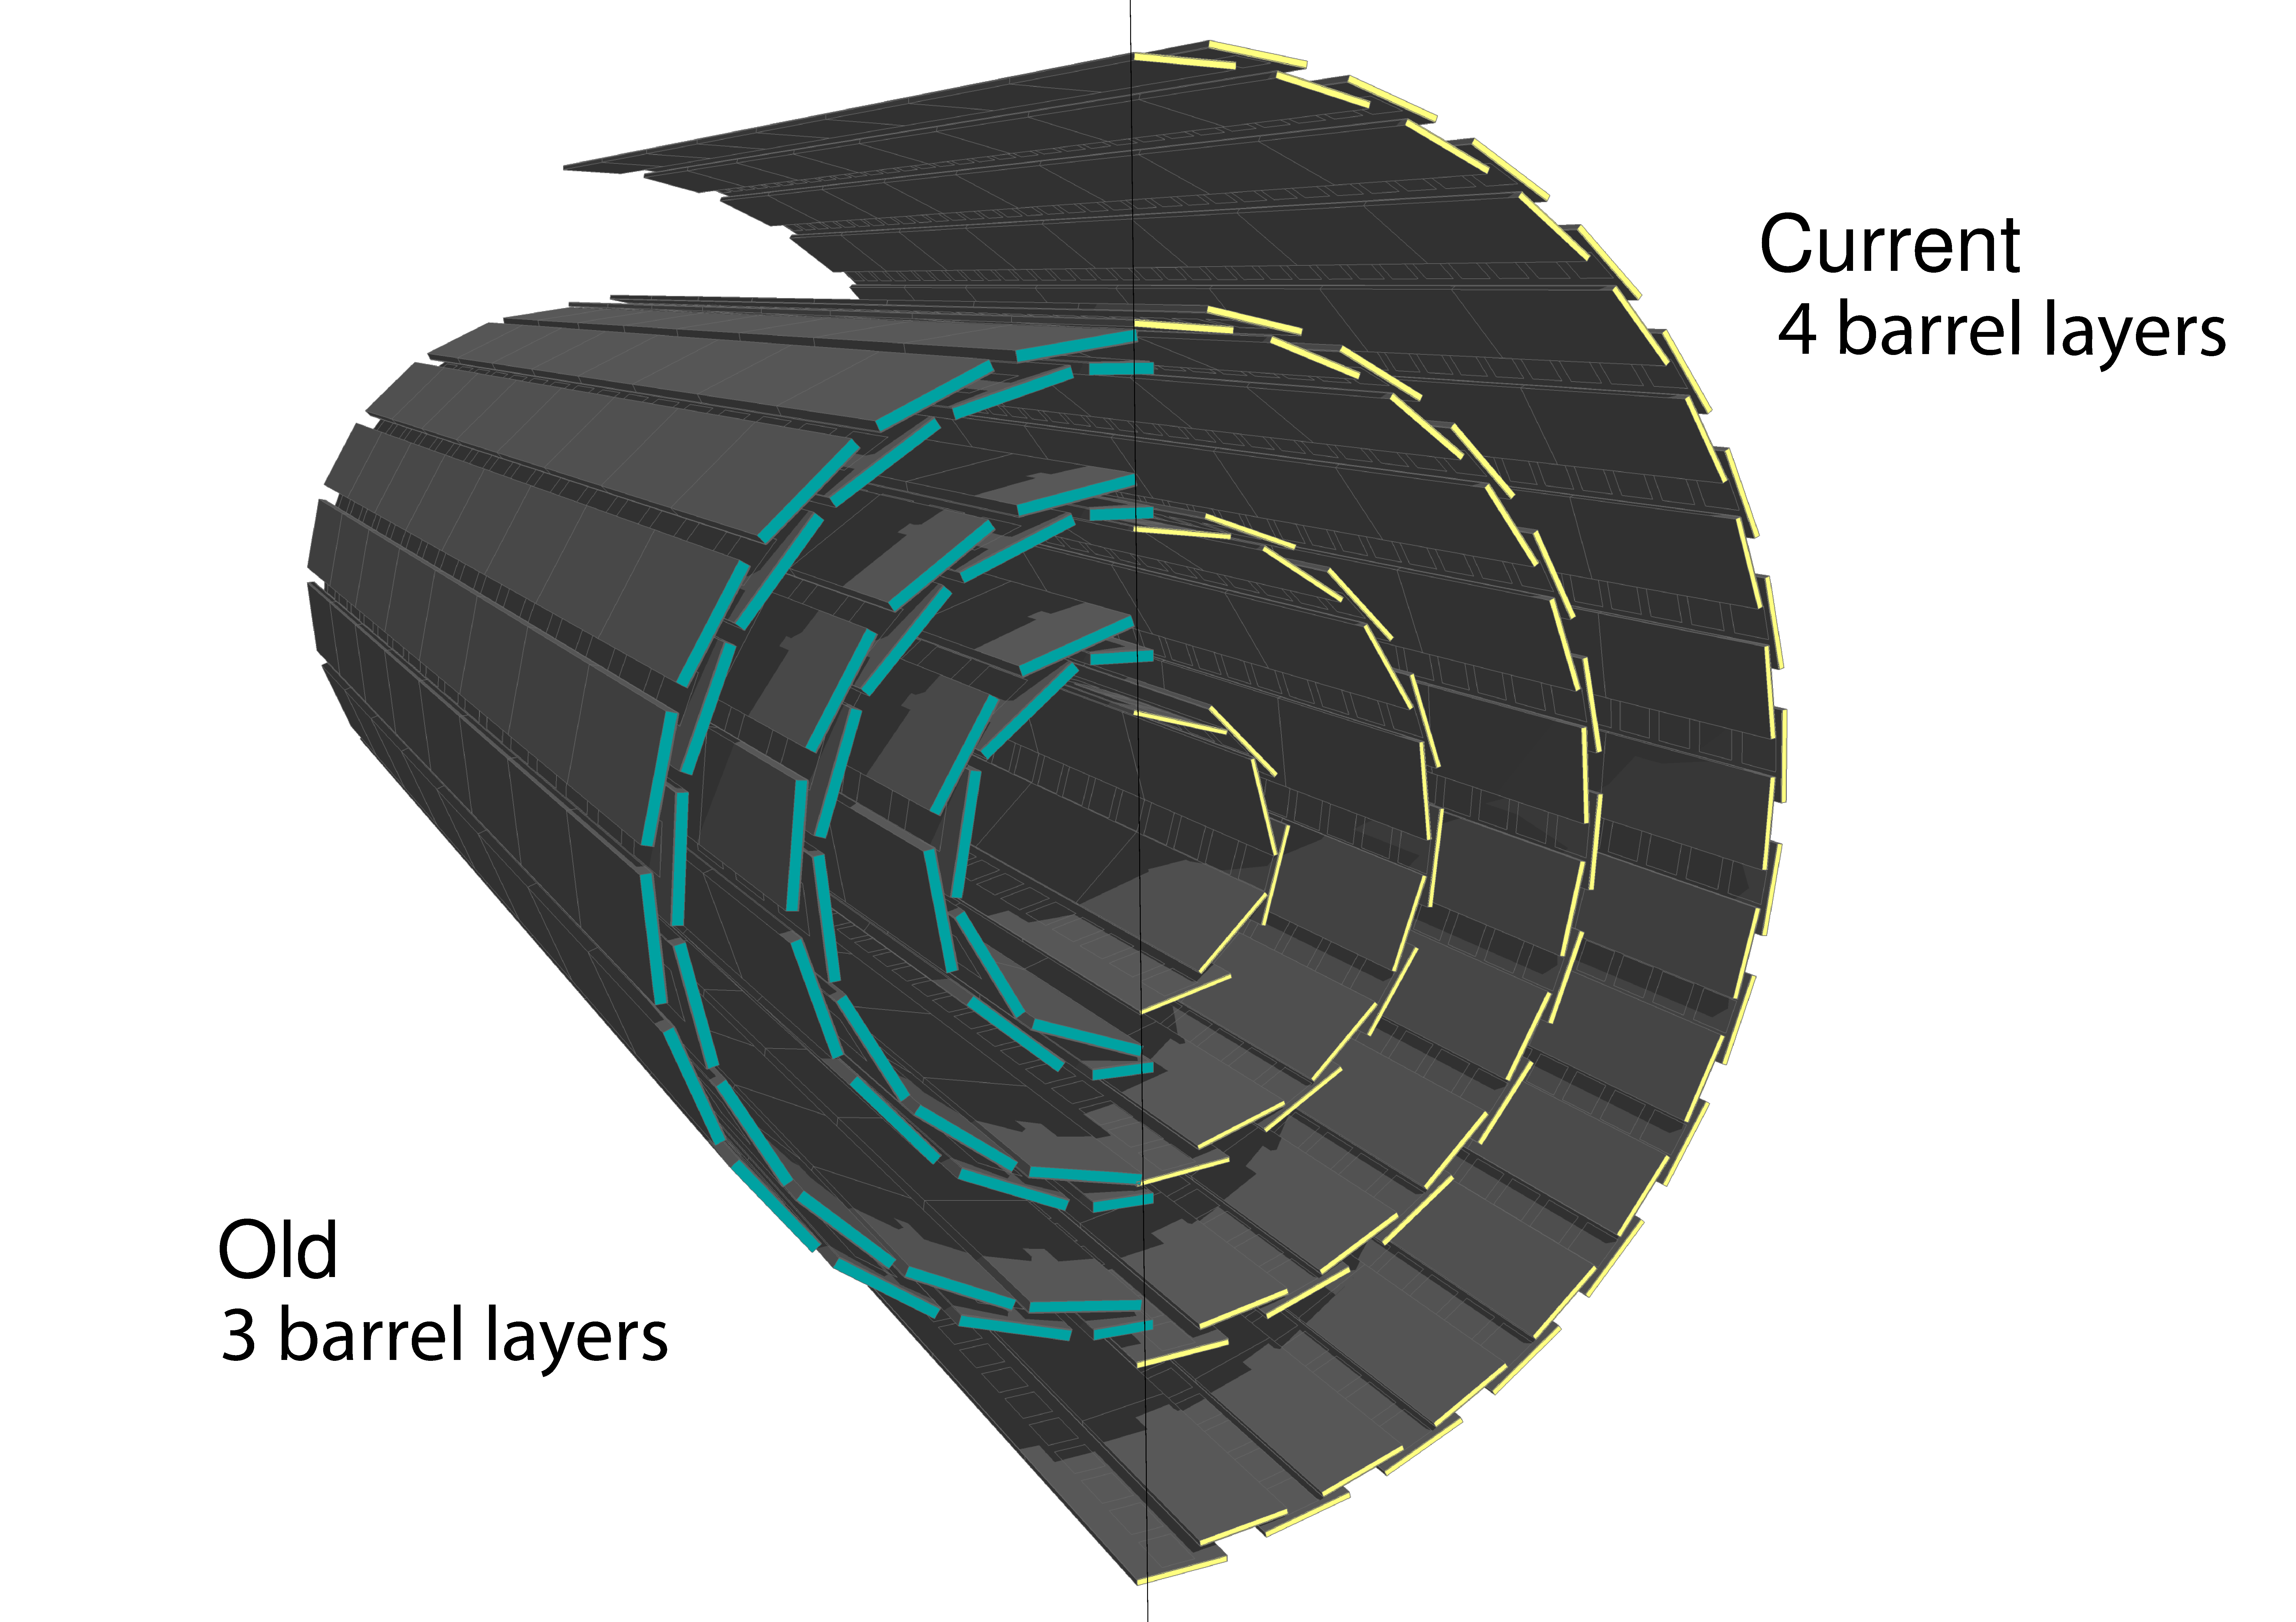
\includegraphics[width=0.39\textwidth]{../images/ch7/bpix.pdf}
\caption[Layout of the upgraded and old pixel detectors.]{Layout and comparison of the layers and disks in the upgraded (Phase I) and old (Phase 0) pixel detectors \cite{pix_tdr}.}\label{fig:new_pix}
\end{figure}

%%%%%%%%%%%%%
%%%%%%%%%%%%
%%%%%%%%%%

\section{Module Production at UNL}
The UNL module production workflow was designed to follow a pipeline-like structure as shown in figure \ref{fig:unlworkflow}. 

\begin{figure}[!h]
  \centering
  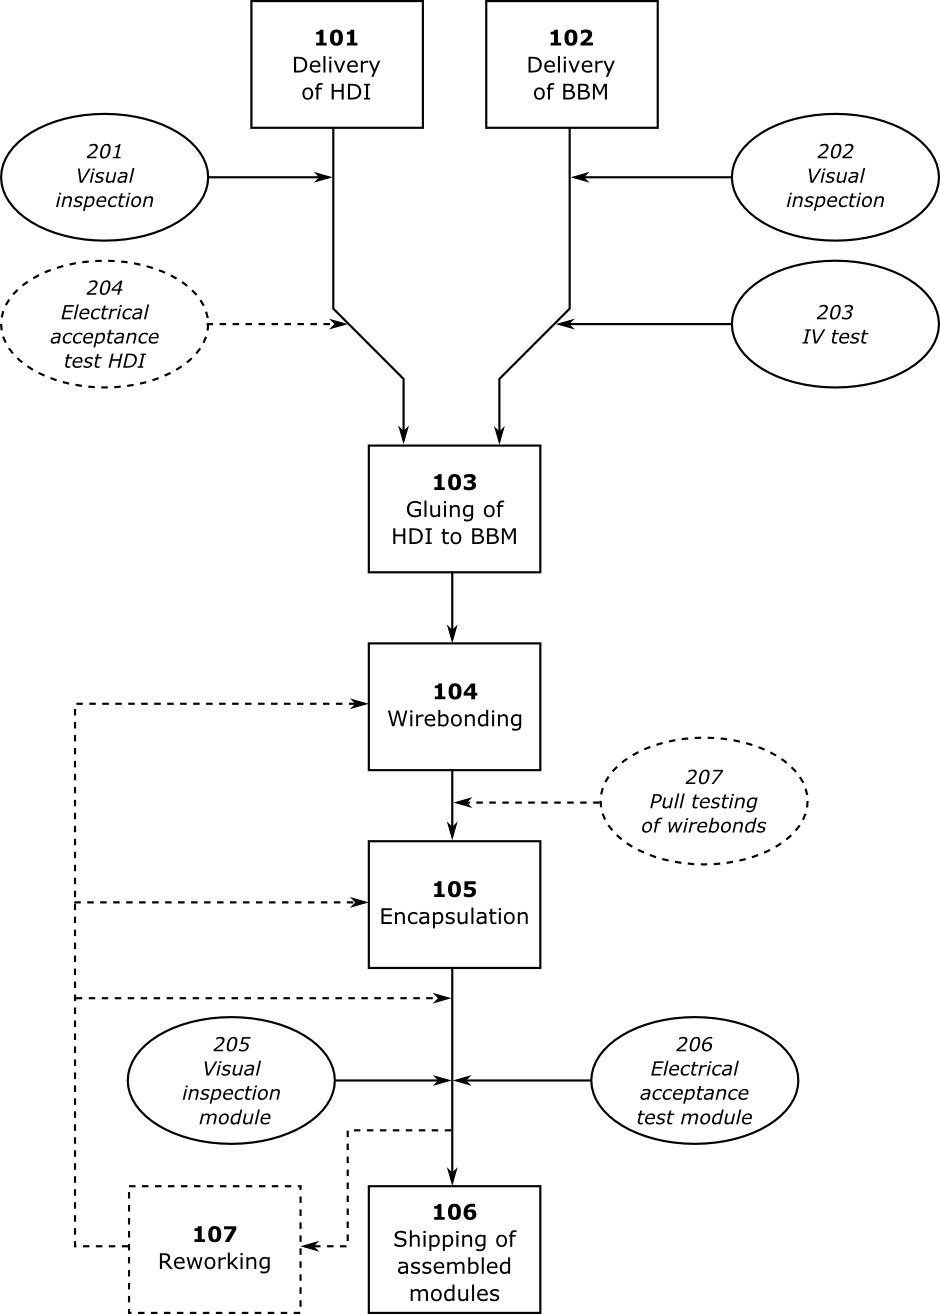
\includegraphics[width=0.7\textwidth]{../images/ch7/unl_workflow}
  \caption[UNL module assembly workflow]{UNL module assembly workflow. Dashed lines represent occasional quality testing and reworking procedures\cite{ph1_sop}.}\label{fig:unlworkflow}
\end{figure}

This allows for different batches of modules to be going through it at different stages without stopping the workflow. Following is a short description of the tests and procedures performed during the production in the UNL silicon Lab. Special emphasis will be made in IV test, visual inspection and electrical test, the stages where the author of this work made most of the work{\rojo{improve}}. 

\subsection{Visual Inspections}
The UNL-HEP group assembly workflow started upon receiving two components: a Bare Bonded Module (BBM) and a High Density Interconnect (HDI), see figure \ref{fig:bbmyhdi}.

\begin{figure}[!h]
\centering
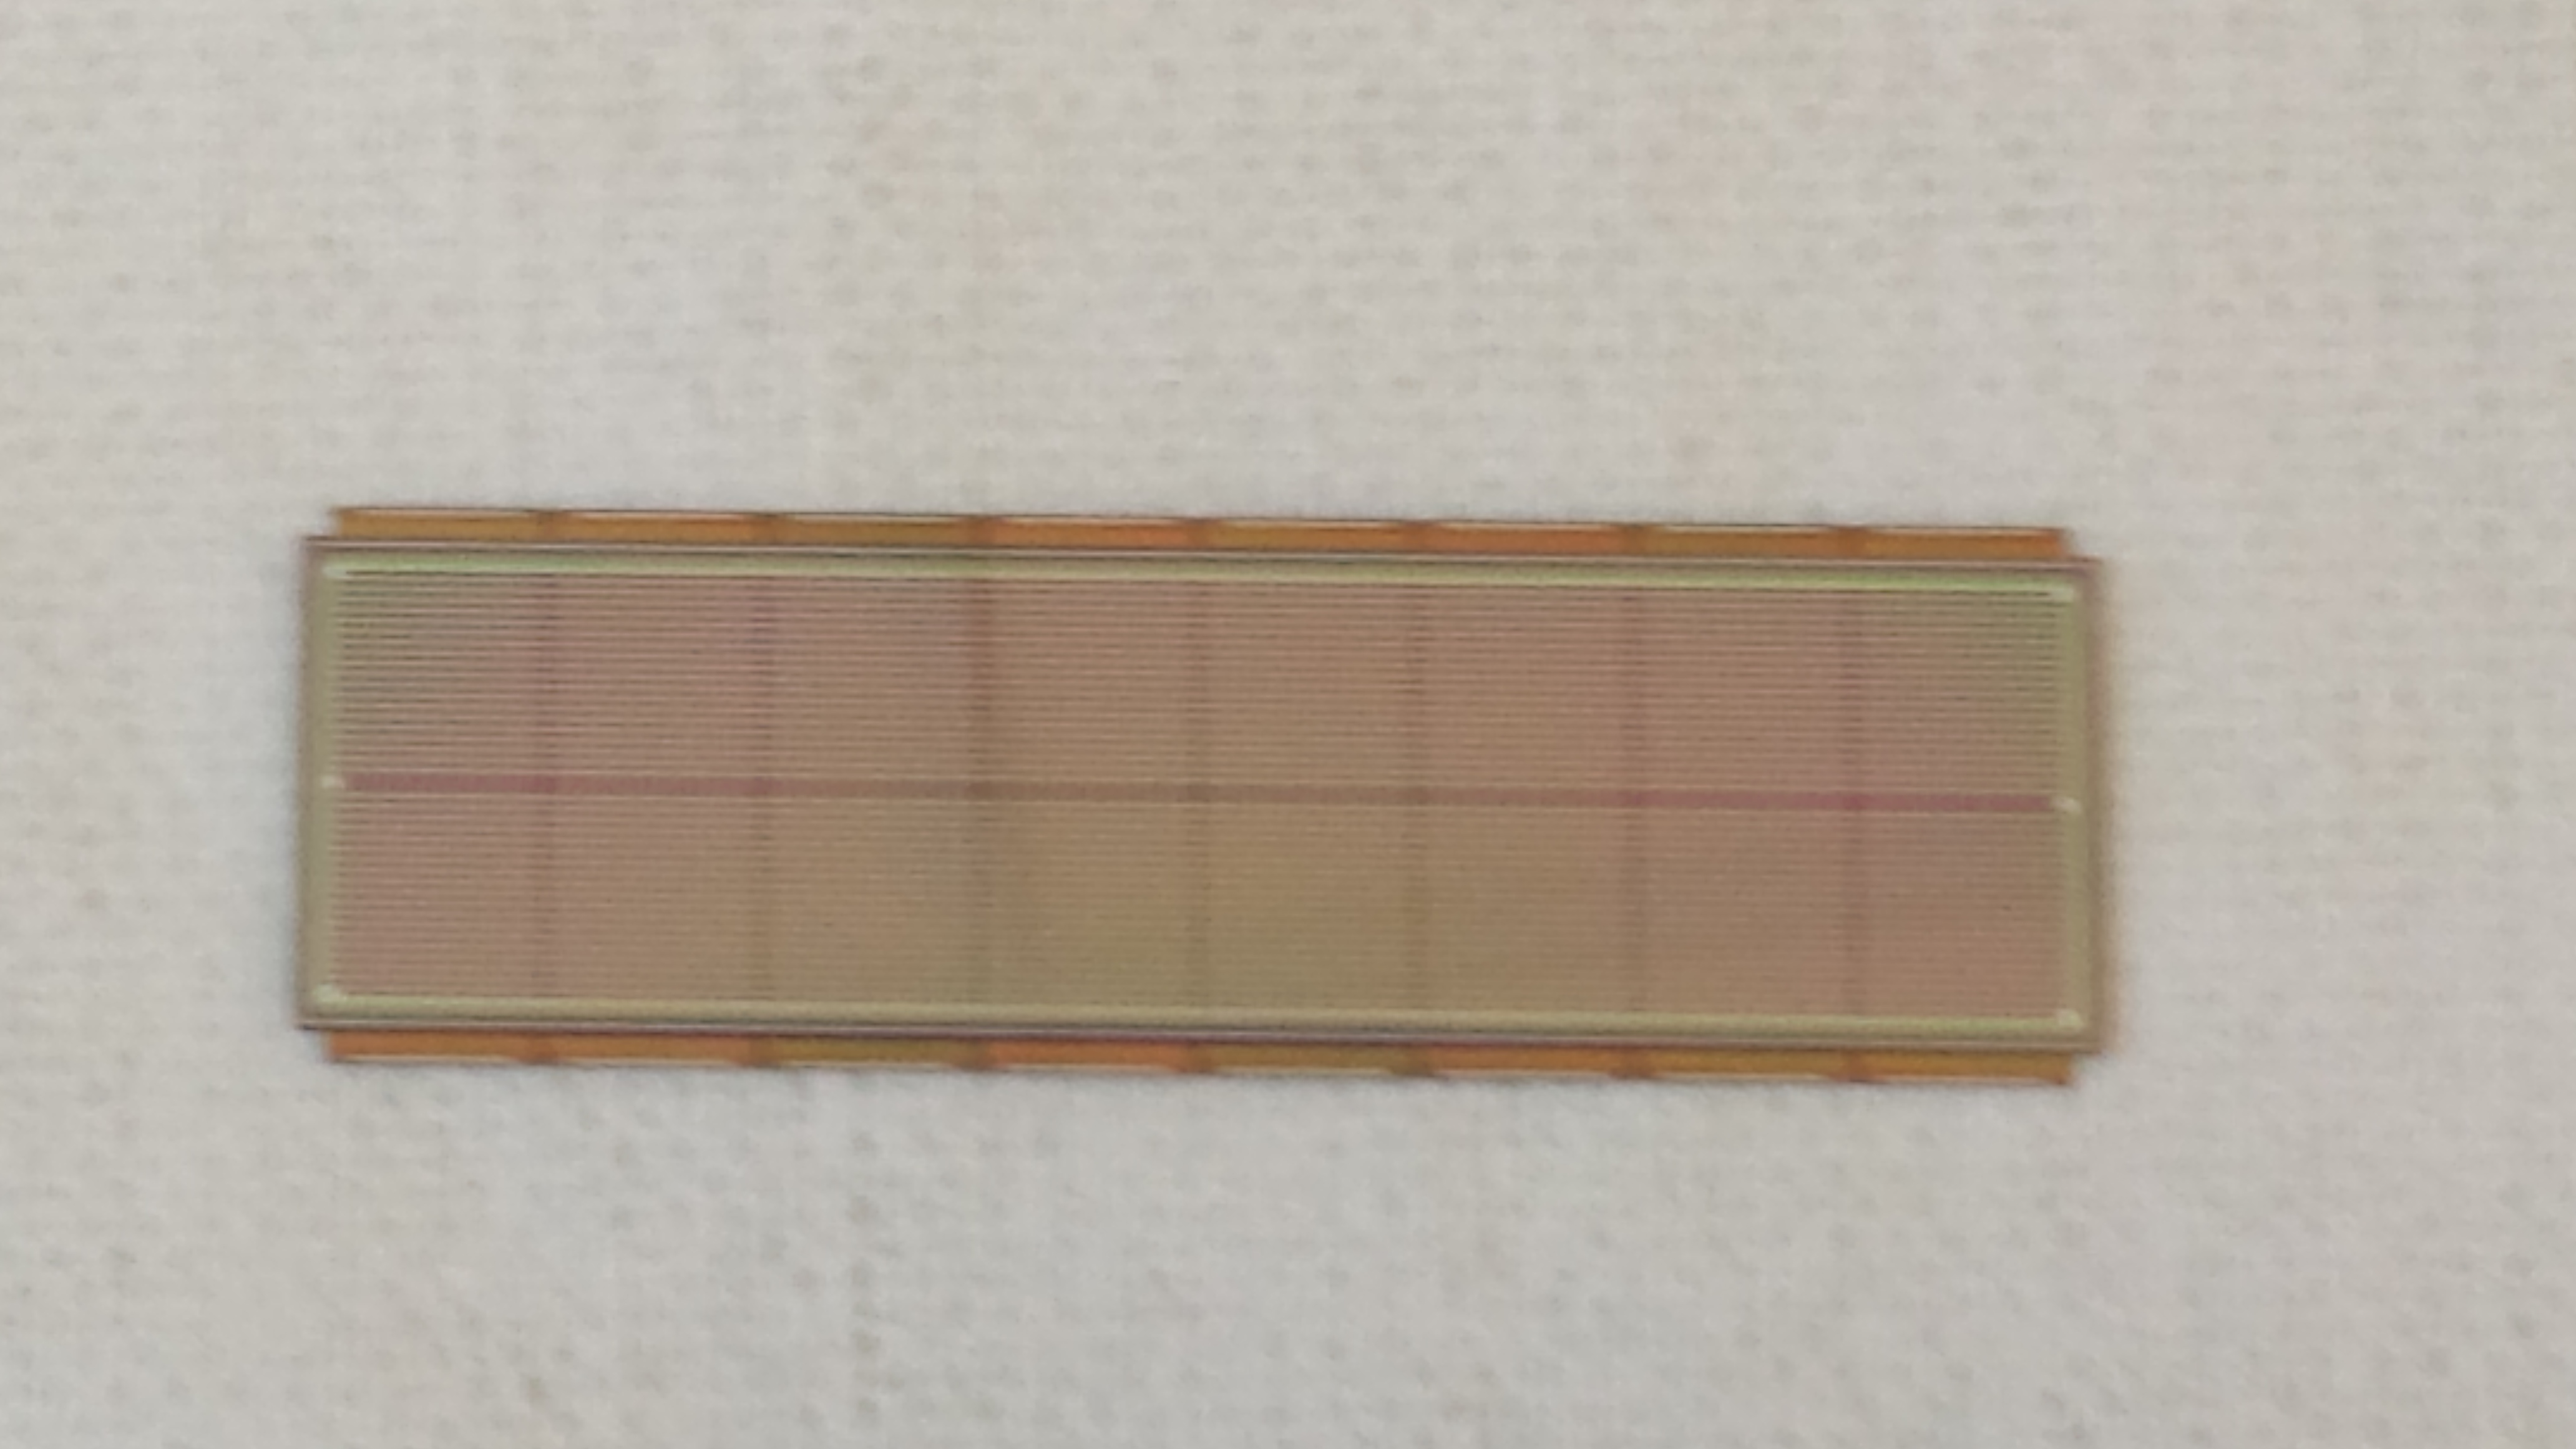
\includegraphics[width=0.6\textwidth]{ch7/bare_module}

\includegraphics[width=0.39\textwidth]{ch7/gato2}
\caption[Photograph of a BBM and HDI.]{Photograph of a BBM (left) and HDI {\rojo{right one}}(right) as received by the UNL-HEP group.}\label{fig:bbmyhdi}
\end{figure}

The first stage of the module production was to do a visual inspection on these components to ensure they were in good conditions and able to continue into the production pipeline. {\rojo{punto aparte?}} To get a good view of such a small components a powerful microscope with magnification of {\rojo{confirm}}, an attached camera, and LED ring illumination was used. A photograph of the set up is shown in figure \ref{fig:probe_station}. The entire set up was connected to a vacuum line to secure these component in place and avoid any damage during the visual inspection. BBM were received in a gel pack while the the HDI were usually received in their modules carriers. BBM and HDI were moved from the container into the probe station using a portable vacuum pen and taking the appropriate safety precaution: ESD wristband, gloves, face mask, etc.

\begin{figure}[!h]
\centering
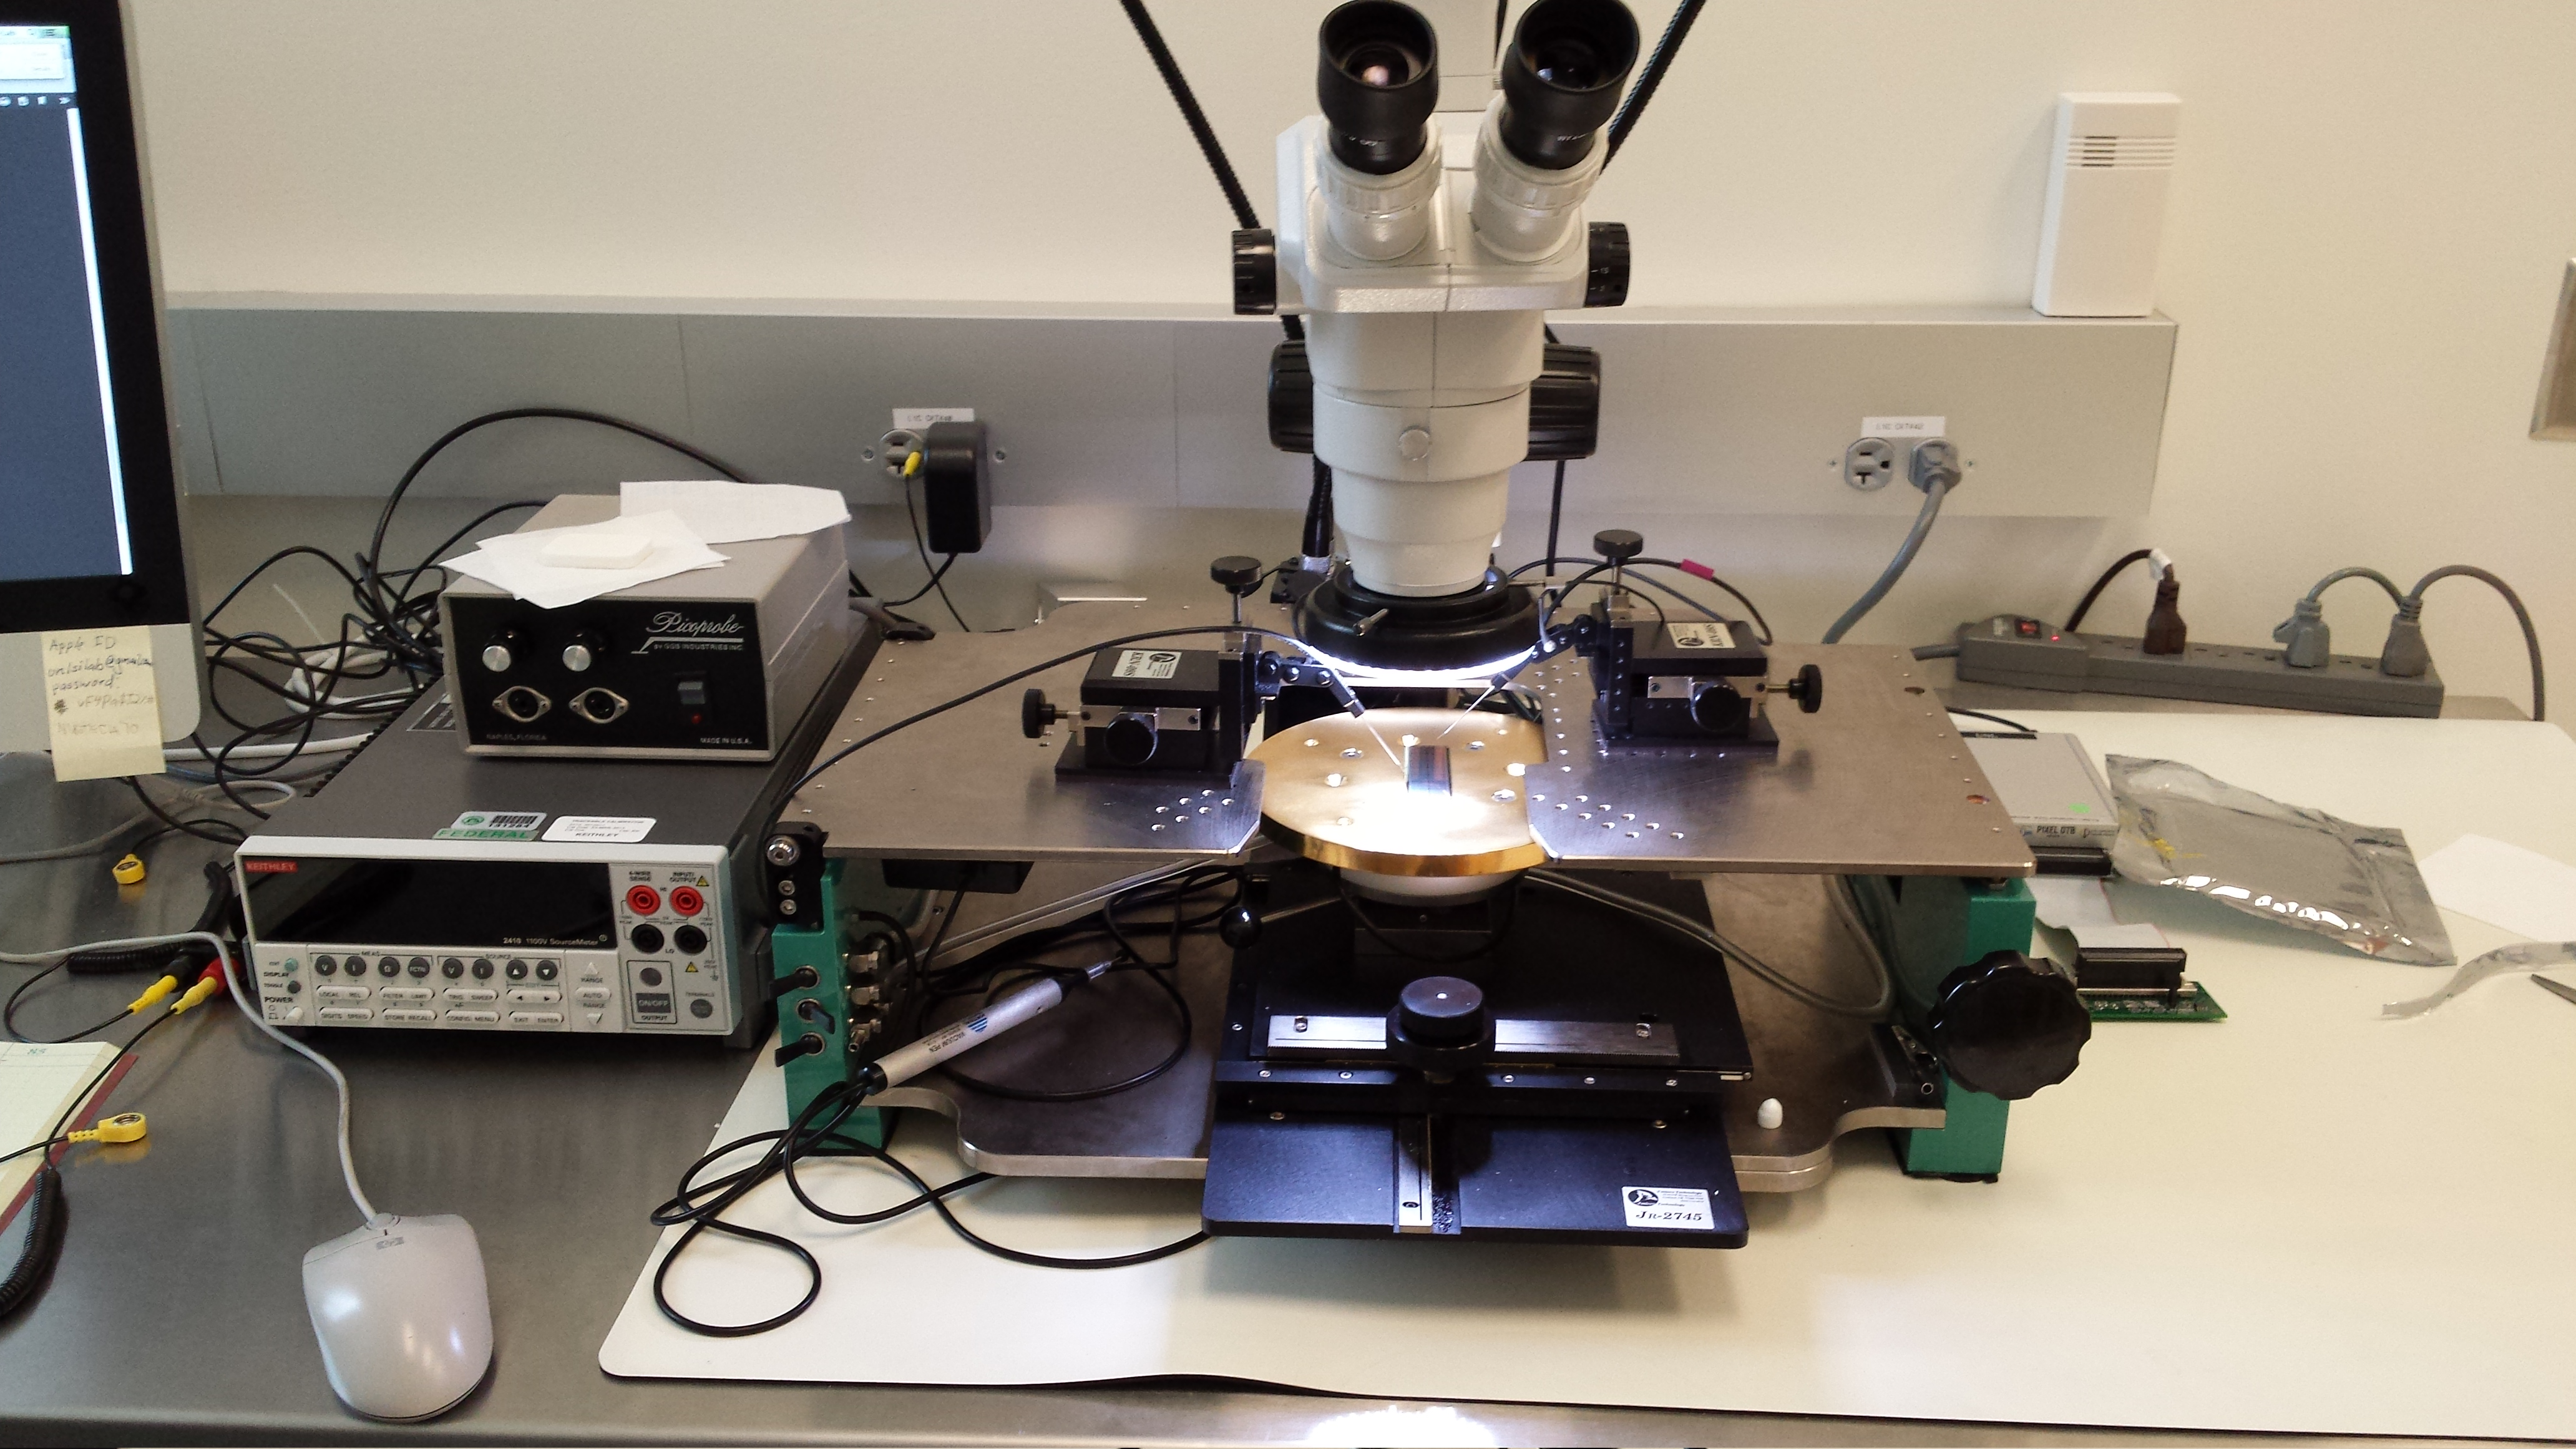
\includegraphics[width=0.7\textwidth]{ch7/probe_station}
\caption[Photograph of the visual inspection and IV test station.]{{\rojo{fix}} Photograph showing a BBM under the microscope during a visual inspection. This station also served as IV test stand.}\label{fig:probe_station}
\end{figure}

During visual inspection BBMs were scanned for unusual features or sign of damage, special attention was given to the high voltage connection and bond pads. Figure \ref{fig:vis_insp_bbm} shows different parts of four different modules where defects are observed {\rojo{defects are on only 3}}. Some of these defects, bottom right figure, caused, the module to be rejected immediately while others, top right and bottom left plots, will still undergo an IV test. While for the HDI the bond pads of the 16 ROCs, the wirebonds of the tbm, and the address pads were carefully checked. Figure \ref{fig:vis_insp_hdi} shows the TBM wirebonds as well as the bondpads of a ROC in a HDI.

\begin{figure}[!h]
  \centering
  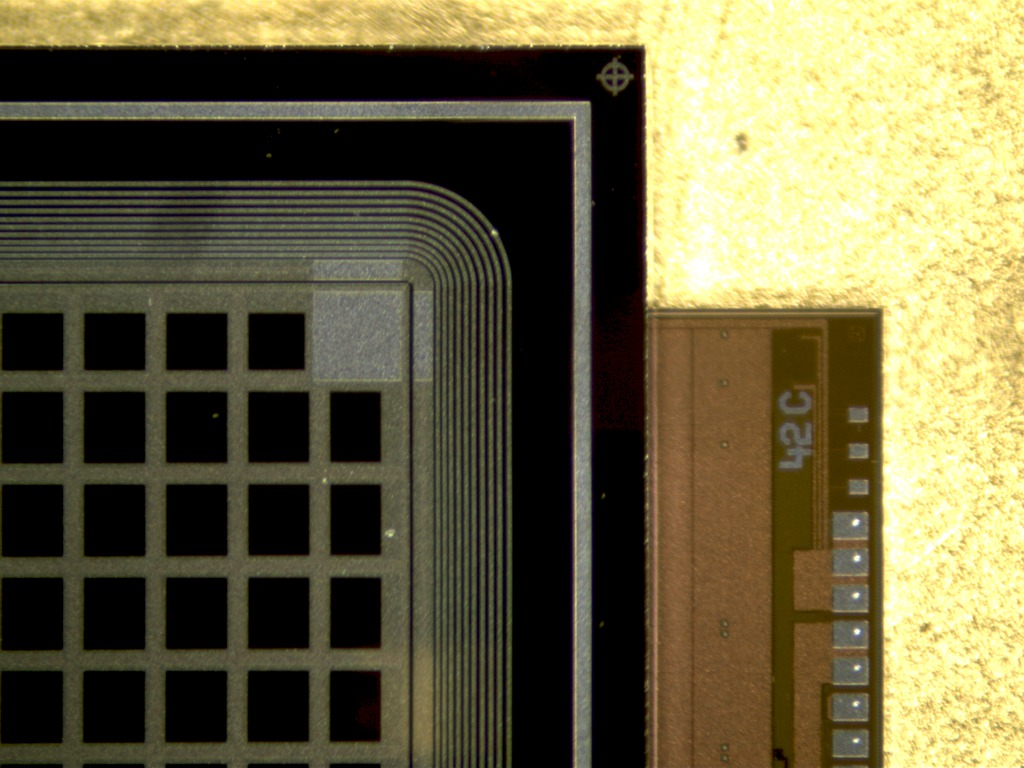
\includegraphics[width=0.4\textwidth]{ch7/vis_insp_1}
  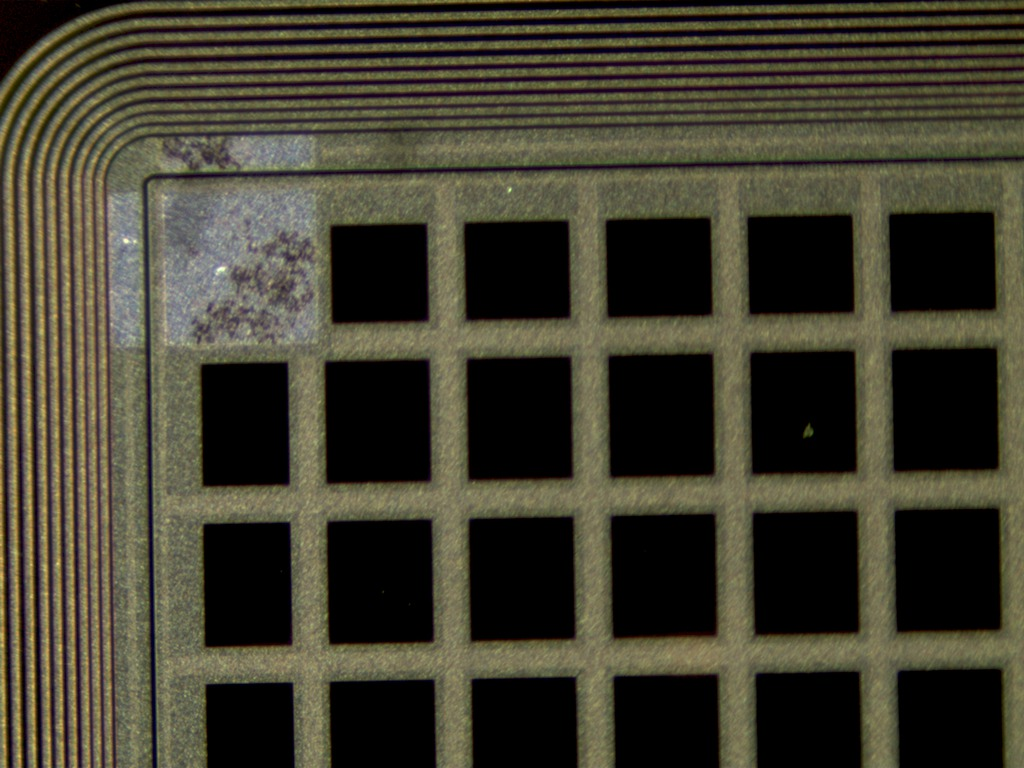
\includegraphics[width=0.4\textwidth]{ch7/vis_insp_2}
  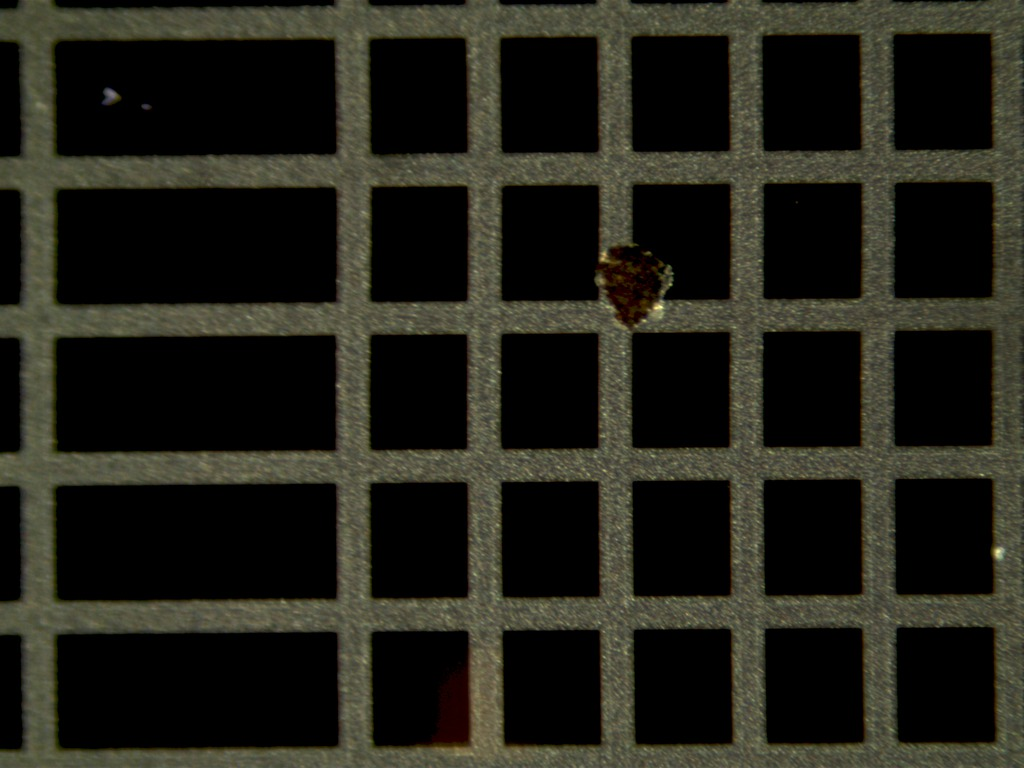
\includegraphics[width=0.4\textwidth]{ch7/vis_insp_3}
  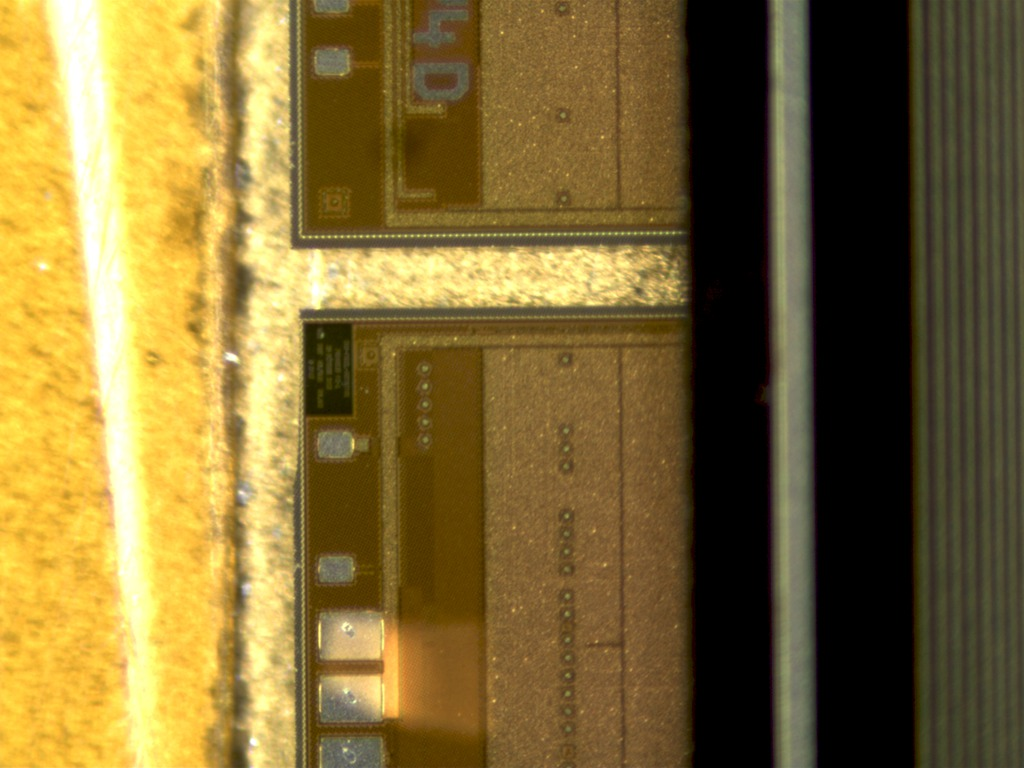
\includegraphics[width=0.4\textwidth]{ch7/vis_insp_5}
  \caption[Visual inspection of a bare module.]{Photograph of the visual inspection of a BBM showing few of the things observed during a visual inspection: A good module (top left), scratches on the high voltage connection path (top right), scratch on the midle of the BBM (bottom left), and scratches on the wire bonds pad (bottom right)}\label{fig:vis_insp_bbm}
\end{figure}

\begin{figure}[!h]
  \centering
  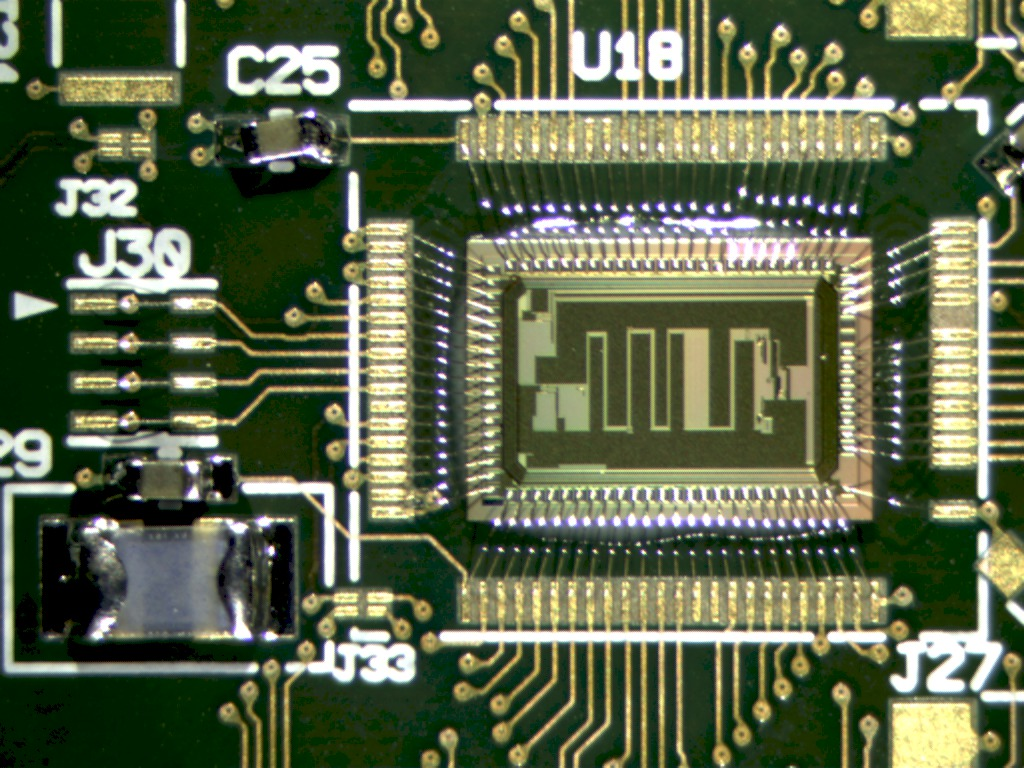
\includegraphics[width=0.4\textwidth]{ch7/hdi_tbm}
  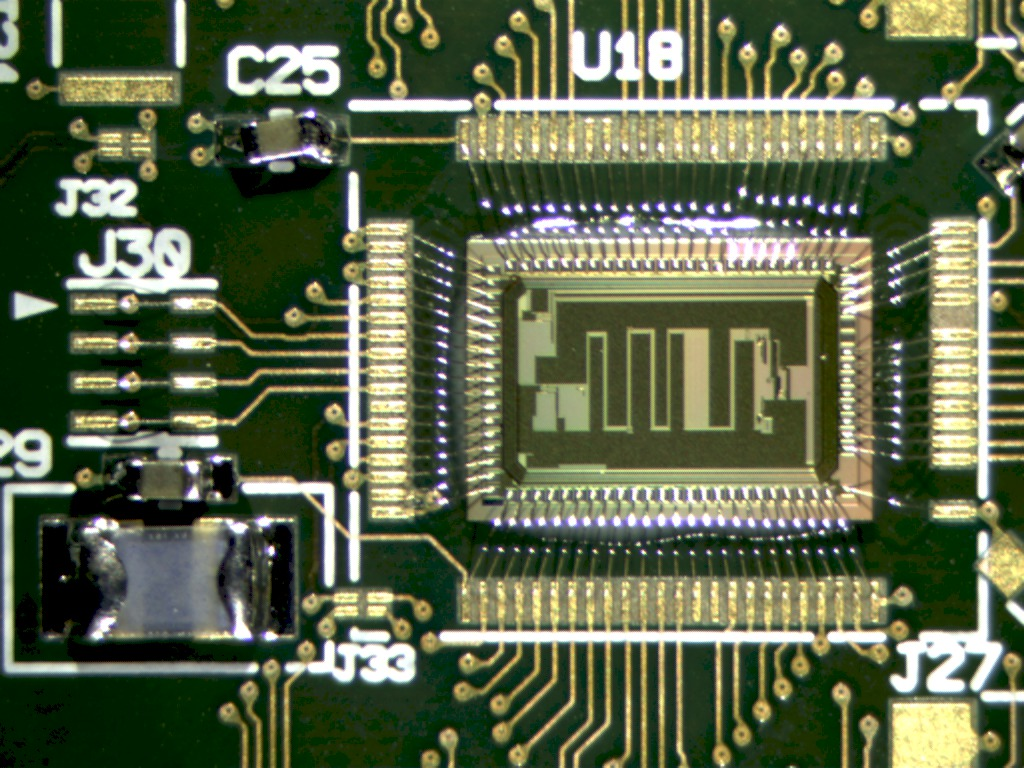
\includegraphics[width=0.4\textwidth]{ch7/hdi_tbm}
  \caption[Visual inspection of a HDI.]{Photograph of the visual inspection of a HDI shwing the wirebonds of the TBM (left) and the bondpads of a ROC (right). {\rojo{right fig}}}\label{fig:vis_insp_hdi}
\end{figure}

Figures \ref{fig:vis_insp_bbm} and Fig. \ref{fig:vis_insp_hdi} show a trend that was observed throughout the entire production. In general more unusual features and damage were observed in BBMs than on HDI. This was because BBM were derivered directly from the production company to our lab while the HDI were delivered to the Fermi National Laboratory (FermiLab) first where they were preliminary tested before the arrived at our testing facilities. 

\subsection{IV Test}\label{ivbbm}
After both BBM and HDI have succesfully passed the visual inspection the BBM continues to the probe station for a current vs voltage (IV) test. The test uses the fact that the sensor behaves like a diode. During operation a potential difference is applied to the sensor to draw the electrons created by a charge particle passing through the sensor towards the bump bond to be collected. If this potential difference is too small not all electron will collected in time and if it is large the sensor could break. This potential difference is known as a depletion voltage. The IV test is meant to find the operating range for a given module (sensor) Figure \ref{fig:iv_test} shows the IV results for a BBM in good condition and figure \ref{fig:sensor_probe_positions} shows the position of the probes to perform an IV on a BBM.  

\begin{figure}[!h]
  \centering
  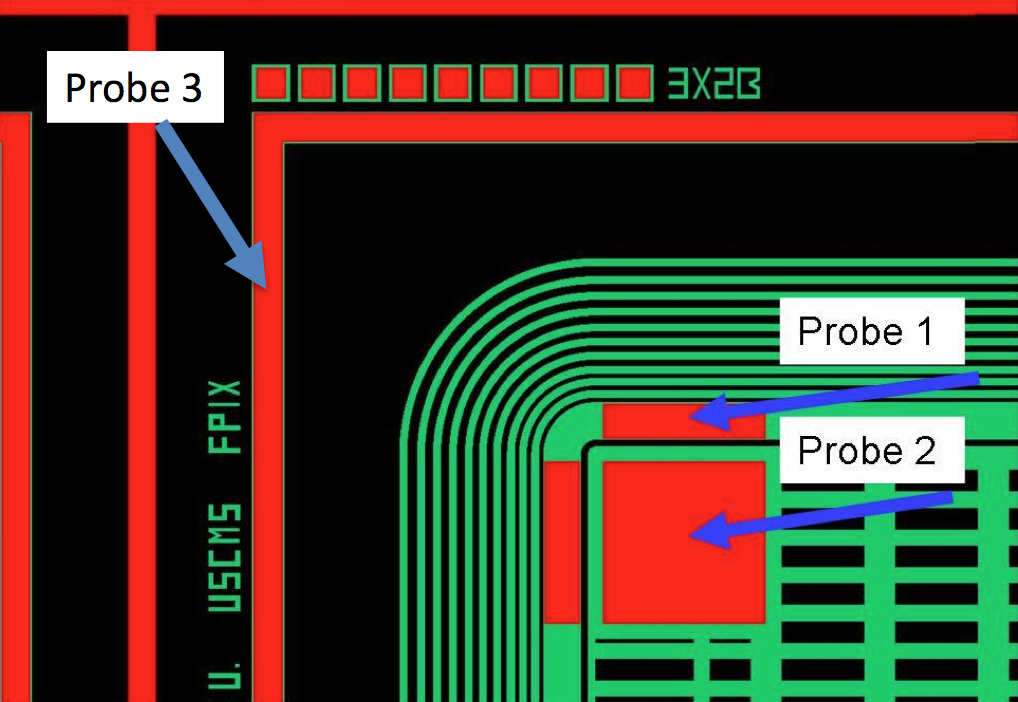
\includegraphics[width=0.5\textwidth]{ch7/sensor_probe_positions}
  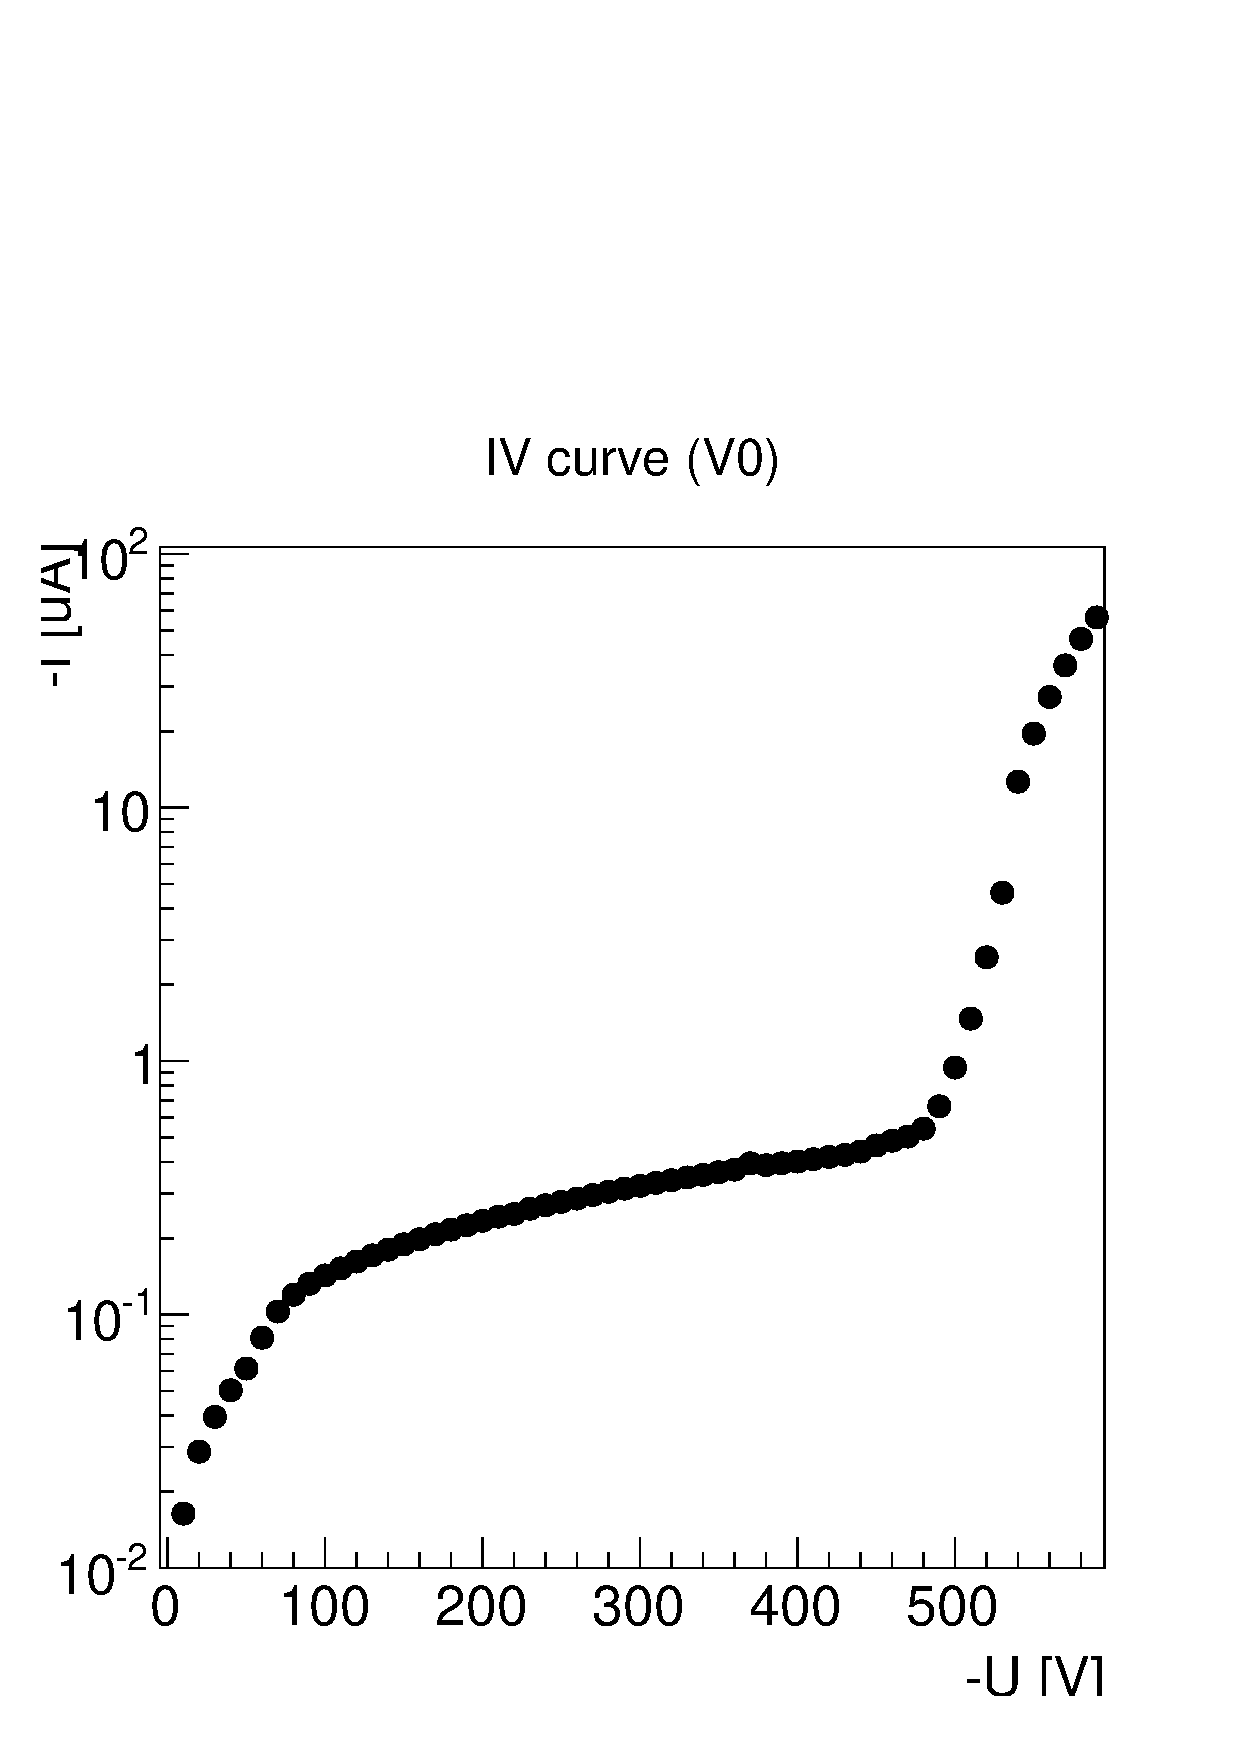
\includegraphics[width=0.4\textwidth]{ch7/iv_test}
  \caption[IV test of BBM]{Left: Probe position for an IV test on a BBM. Probe 2 is high voltage, probe 3 is ground, and probe 1 was not used \cite{ph1_sop}. Right: IV test results for a good BBM. The depletion voltage for this module is around {\rojo{confirm with right picture}}.}\label{fig:sensor_probe_positions}
\end{figure}

%{\rojo{why bbm has lower compliance?}}









\subsection{Gluing}
The gluing routine was carefully design to perfectly match the HDI and BBM bondpads. This stage of the production was done using a custom made gantry \ital{AGS15000 Series Gantry}, fabricated by Aerotech \cite{aerotech}. It offered translational motion in 3D as well as rotation in x-y (gantry table) plane. A camera was attached to the gantry head allowing the user to monitor the entire process. This camera was of particular importance during the development and improvement of the gluing routine. A video showing the gluing routine in action can be watched at \cite{gluing_frank} and a full description of the gluing routine and procedure can be found in \cite{and_the}. Figure \ref{fig:gantry} shows the gantry with the different tools used to glue a HDI on a BBM. The final product after the process in complete can be seen in Fig. \ref{fig:hdionbbm}.

\begin{figure}[!h]
  \centering
  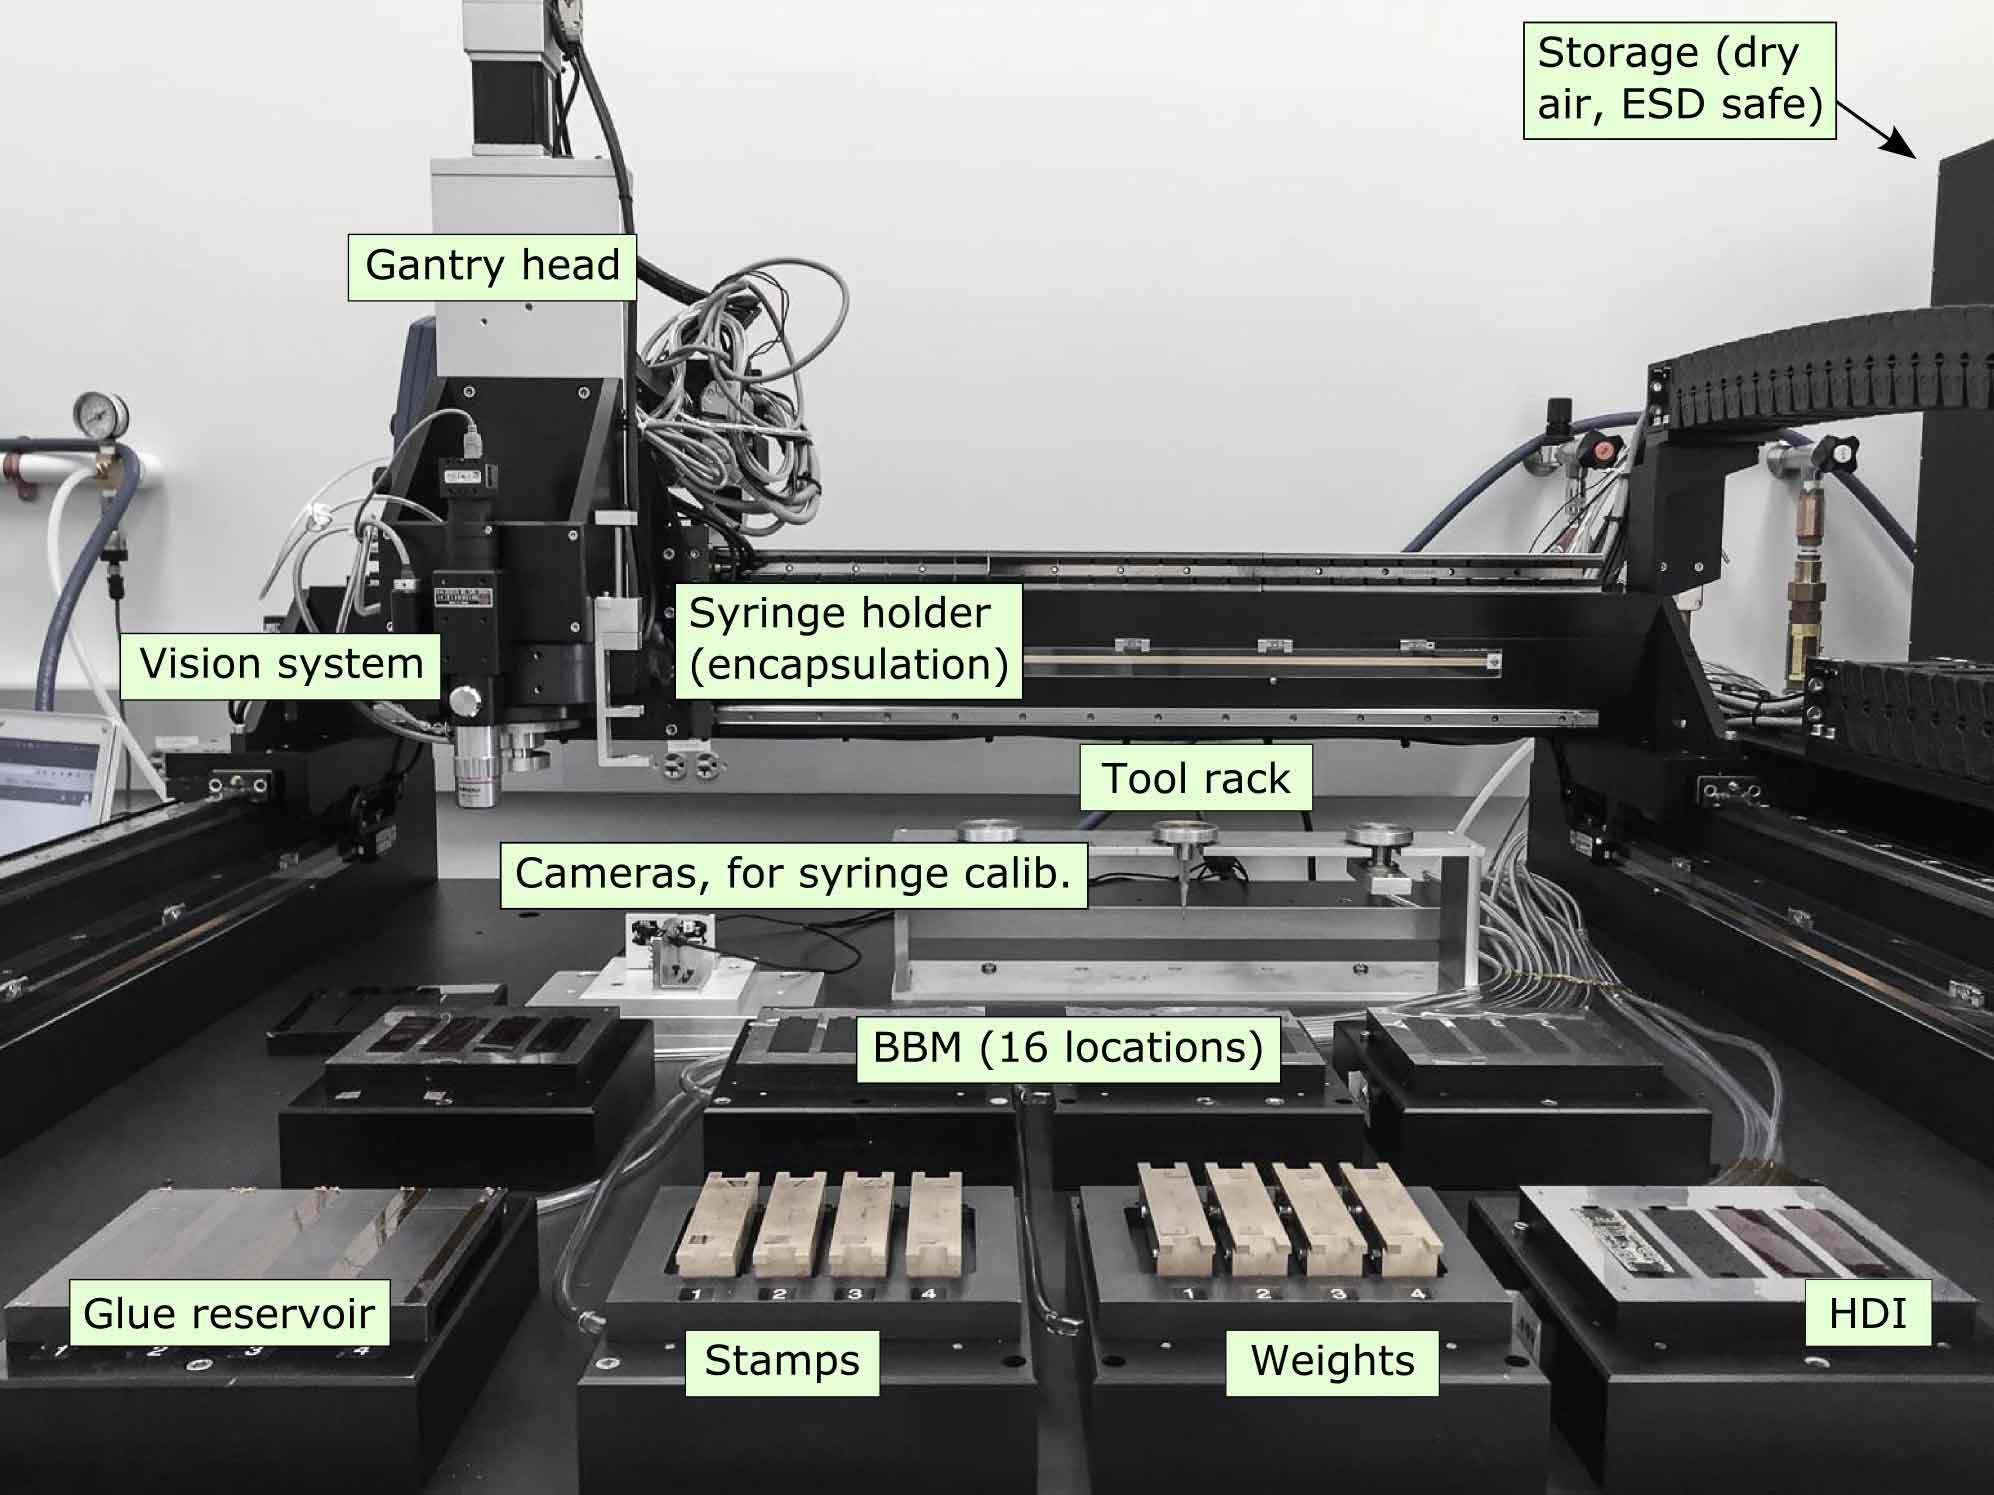
\includegraphics[width=0.7\textwidth]{ch7/gantry}
  \caption[Gluing and encapsulation set up]{Photograph of a gantry used for gluing and encapsulation showing different parts of the set up and tools. }\label{fig:gantry}
\end{figure}

\begin{figure}[!h]
  \centering
  \includegraphics[width=0.5\textwidth]{ch7/hdi_on_bbm}
  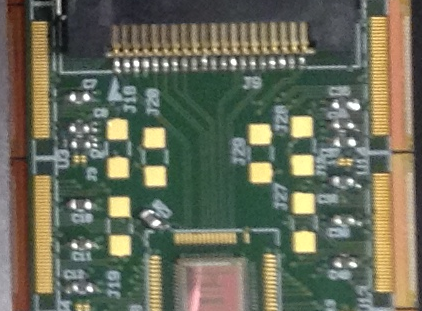
\includegraphics[width=0.5\textwidth]{ch7/hdi_on_bbm_close}
  \caption[Gluing result]{HDI glued on top of a BBM. For a batch of four modules (top) zoom in view to note the almost perfect alignment between the HDI and BBM bondpads.}\label{fig:hdionbbm}
\end{figure}








\subsection{Wirebonding}
After an HDI is glued to a BBM the next step in the assembly process is to make electrical connection between them. 

\begin{figure}[!h]
  \centering
  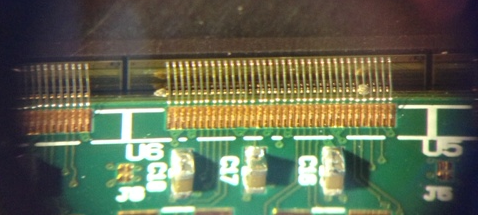
\includegraphics[width=0.7\textwidth]{ch7/wirebonder}
  \caption[wirebonder machine]{Wirebonding set up.}\label{fig:wirebonder}
\end{figure}


\begin{figure}[!h]
  \centering
  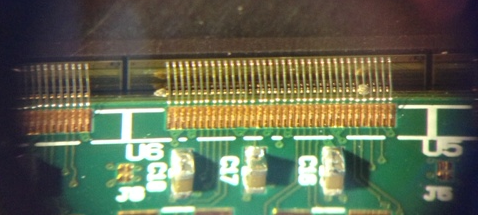
\includegraphics[width=0.7\textwidth]{ch7/wirebond}
  \caption[Wirebonded module]{Close up view of the wirebonds for a single ROC on a wirebonded module.}\label{fig:wirebond}
\end{figure}



\subsection{Encapsulation}
The final step in manufacturing a module is to protect (cover) the wirebonds with an encapsulant, wirebond encapsulation. This procedure is necessary to ensure that the wirebonds are secure at both HDI and BBM ends. The set up and the equipment used is the same as for gluing showed in figure \ref{fig:gantry} and additional materials needed for this step are shown in figure \ref{fig:encapmate}. 
 
\begin{figure}[!h]
  \centering
  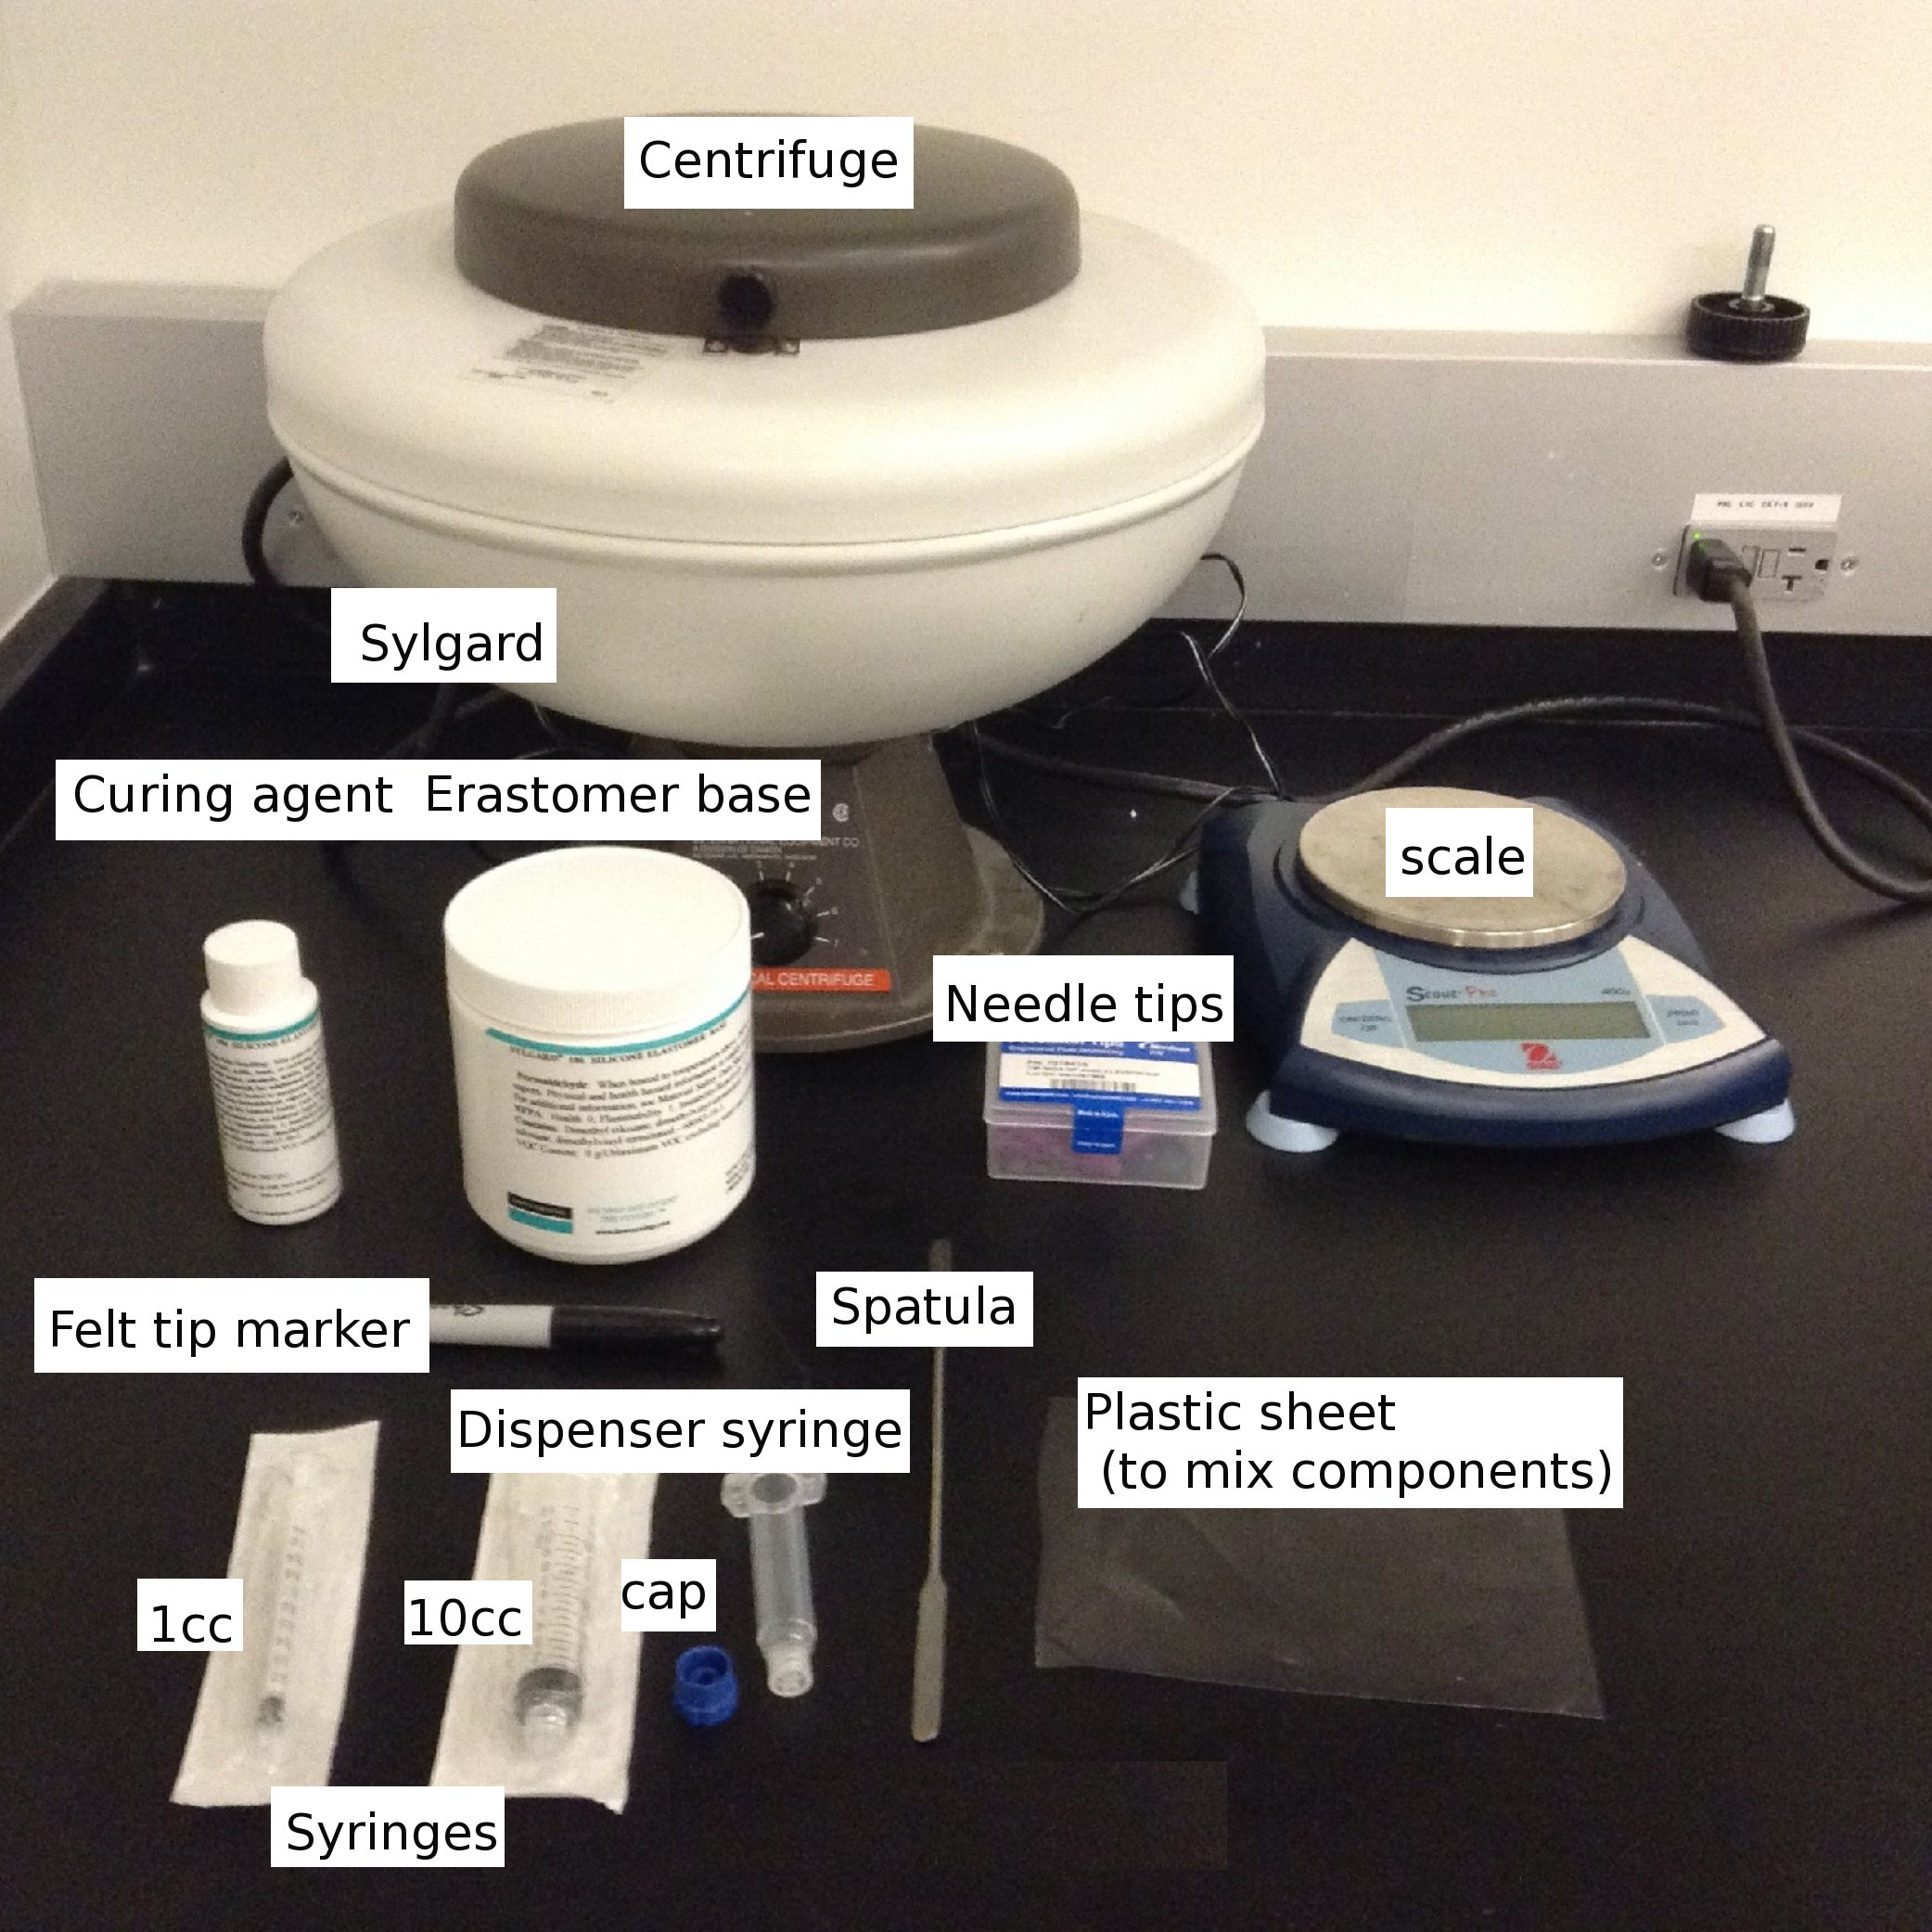
\includegraphics[width=0.5\textwidth]{ch7/encap_mat}
  \caption[Encapsulation materials]{Wirebonds encapsulation materials \cite{ph1_sop}.}\label{fig:encapmate}
\end{figure}

A material suitable for this task must be radiation hard and lightweight among other properties. After testing different material and alloys we settle on \ital{Silgard 186}, a mixture of two-component encapsulant. Erastomer (10 cc) and elastomer (1 cc) base and curing agent respectively. The components were then mix together using a centriguge and place in syringes for dispensing. Figure \ref{fig:encap} shows a module after its different components have been encapsulated. Note how all bond foots and pads are fully covered as needed. 

\begin{figure}[!h]
  \centering
  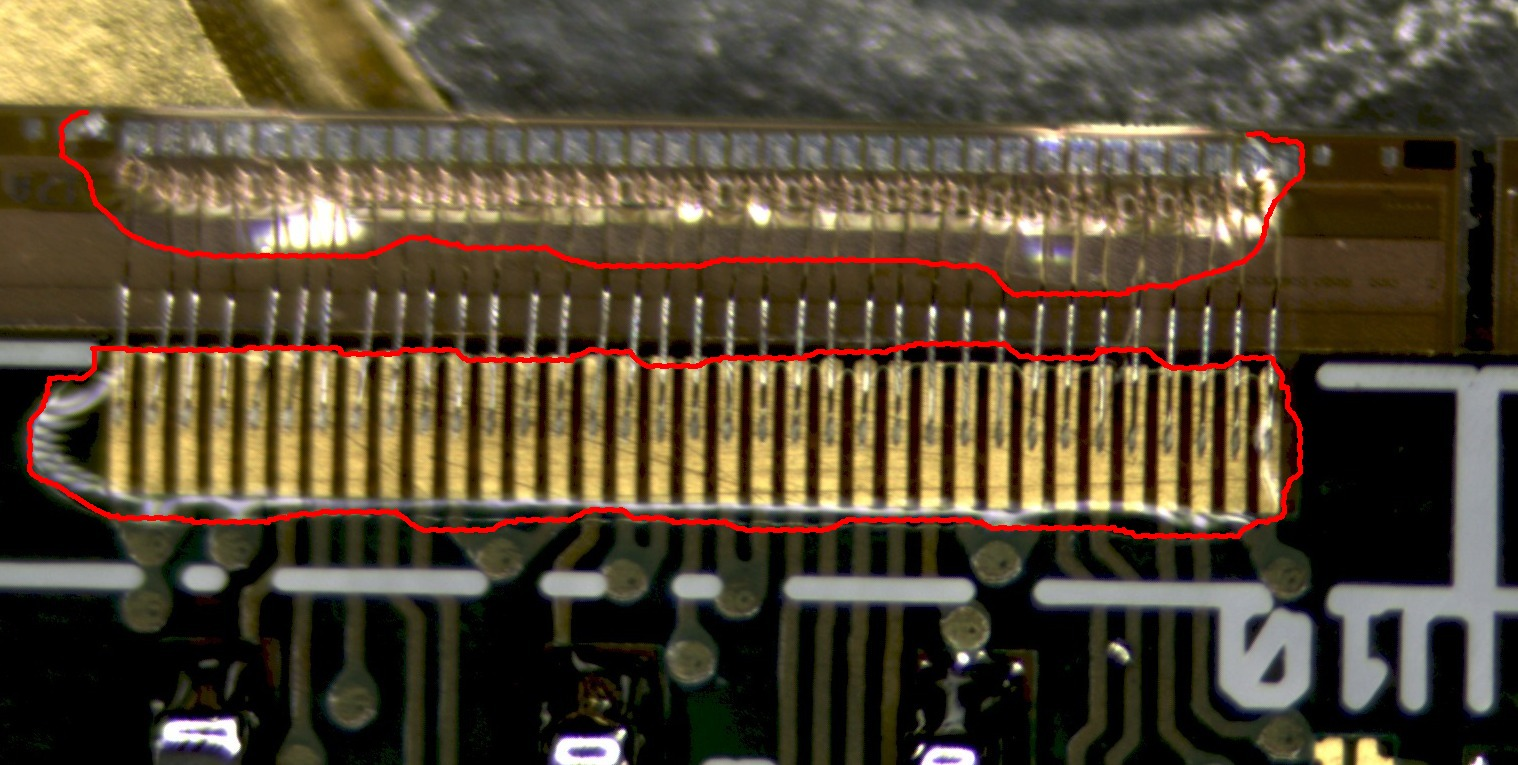
\includegraphics[width=0.5\textwidth]{ch7/encap_ref}
  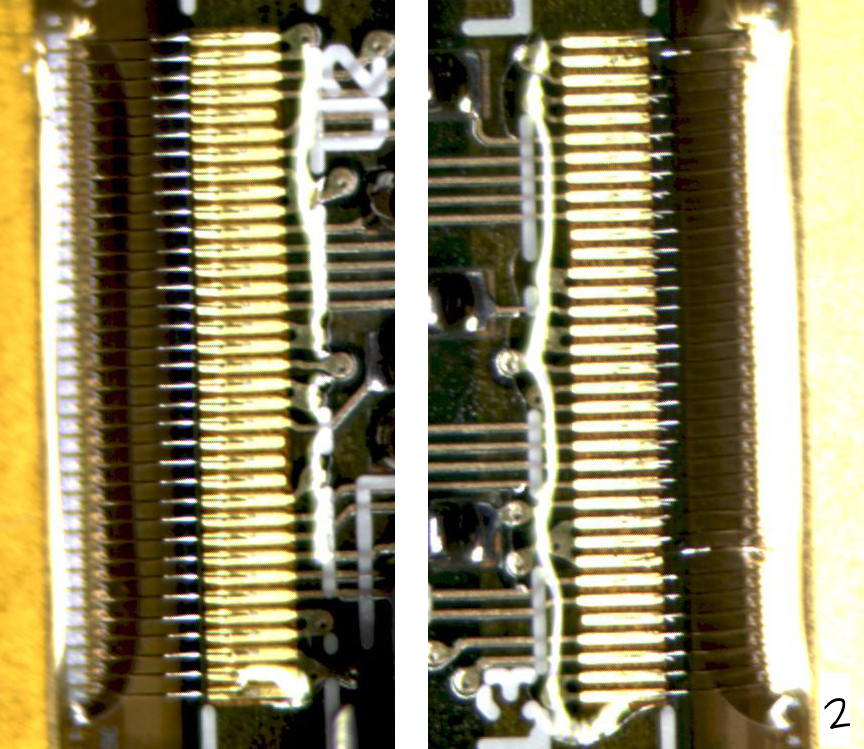
\includegraphics[width=0.4\textwidth]{ch7/encap_roc}
  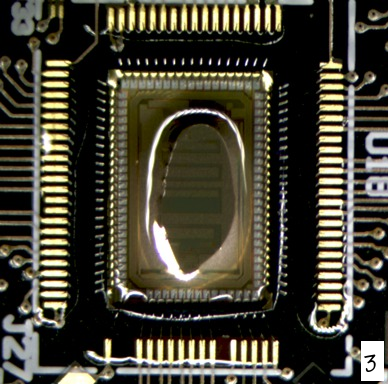
\includegraphics[width=0.2\textwidth]{ch7/encap_tbm}
  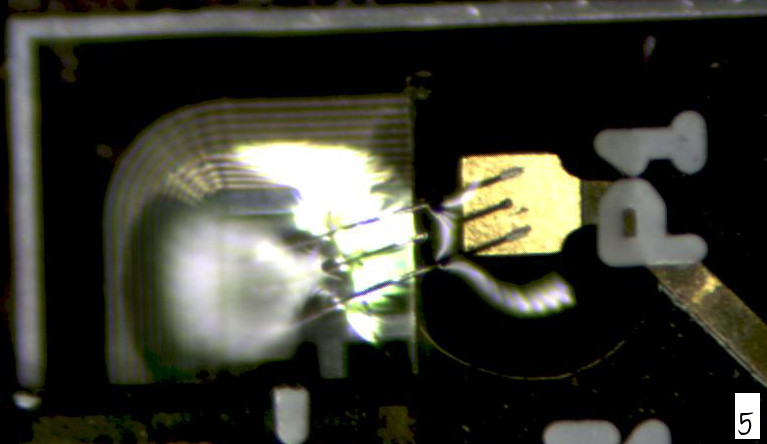
\includegraphics[width=0.4\textwidth]{ch7/encap_hv}
  \caption[Encapsulation results]{Wirebonds encapsulation of the components of a module. Top left, roc used as reference, the boundaries of the encapsulant are enhanced with red lines for better visibility. Top right, two ROCs on two different modules side by side, b) encapsulation of TBM, c) encapsulation of the high voltage pad.}\label{fig:encap}
\end{figure}

\subsection{Electrical Test of a Fully assembly Module}
A manufactured module can be seen in Figure \ref{fig:fully_asem_mod}, it is then visually inspected and mark as ready for electrical test {\rojo{at the end of previous session?}}. 
The electrical test of a fully assembly modules are done using the \ital{pXar} software framework. More information on pXar can be found at \cite{pxar}. The objective of the electrical test is to ensure that all 16 ROCs were functional and have good performance. For this purpose a suit of several tests were designed and developed, the software is flexible in the sense that we could execute a single test just by calling it or we could execute them all with a single command usually referred to as \ital{fulltest}. 
The following section {\rojo{subsections?}} give a short description of the most \ital{important} tests a module has to surpass as well as the output of said test. A full list of the tests, a comprehensive description of them, and a {\rojo{description}} of their purpose can be found in \cite{fpix_module_testing_guide} and references therein. 

\begin{figure}[!h]
  \centering
  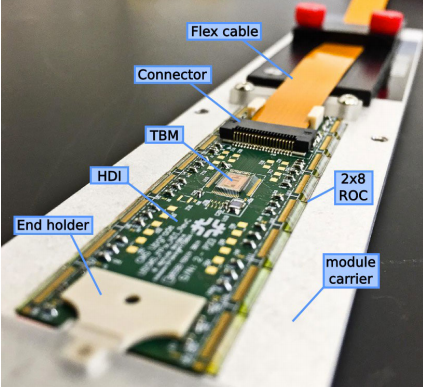
\includegraphics[width=0.7\textwidth]{../images/ch7/fully_asem_mod}
  \caption[Fully assembly Module]{Fully assembly Module}\label{fig:fully_asem_mod}
\end{figure}

\subsubsection{IV Test}
A fully assembled module also undergoes an IV test as described in \ref{ivbbm}. The primary purpose of this test is to ensure that not damage was done to the circuitry during the assembly process. The IV result for a sample module is shown in figure \ref{ivfullmod}

\begin{figure}[!h]
  \centering
  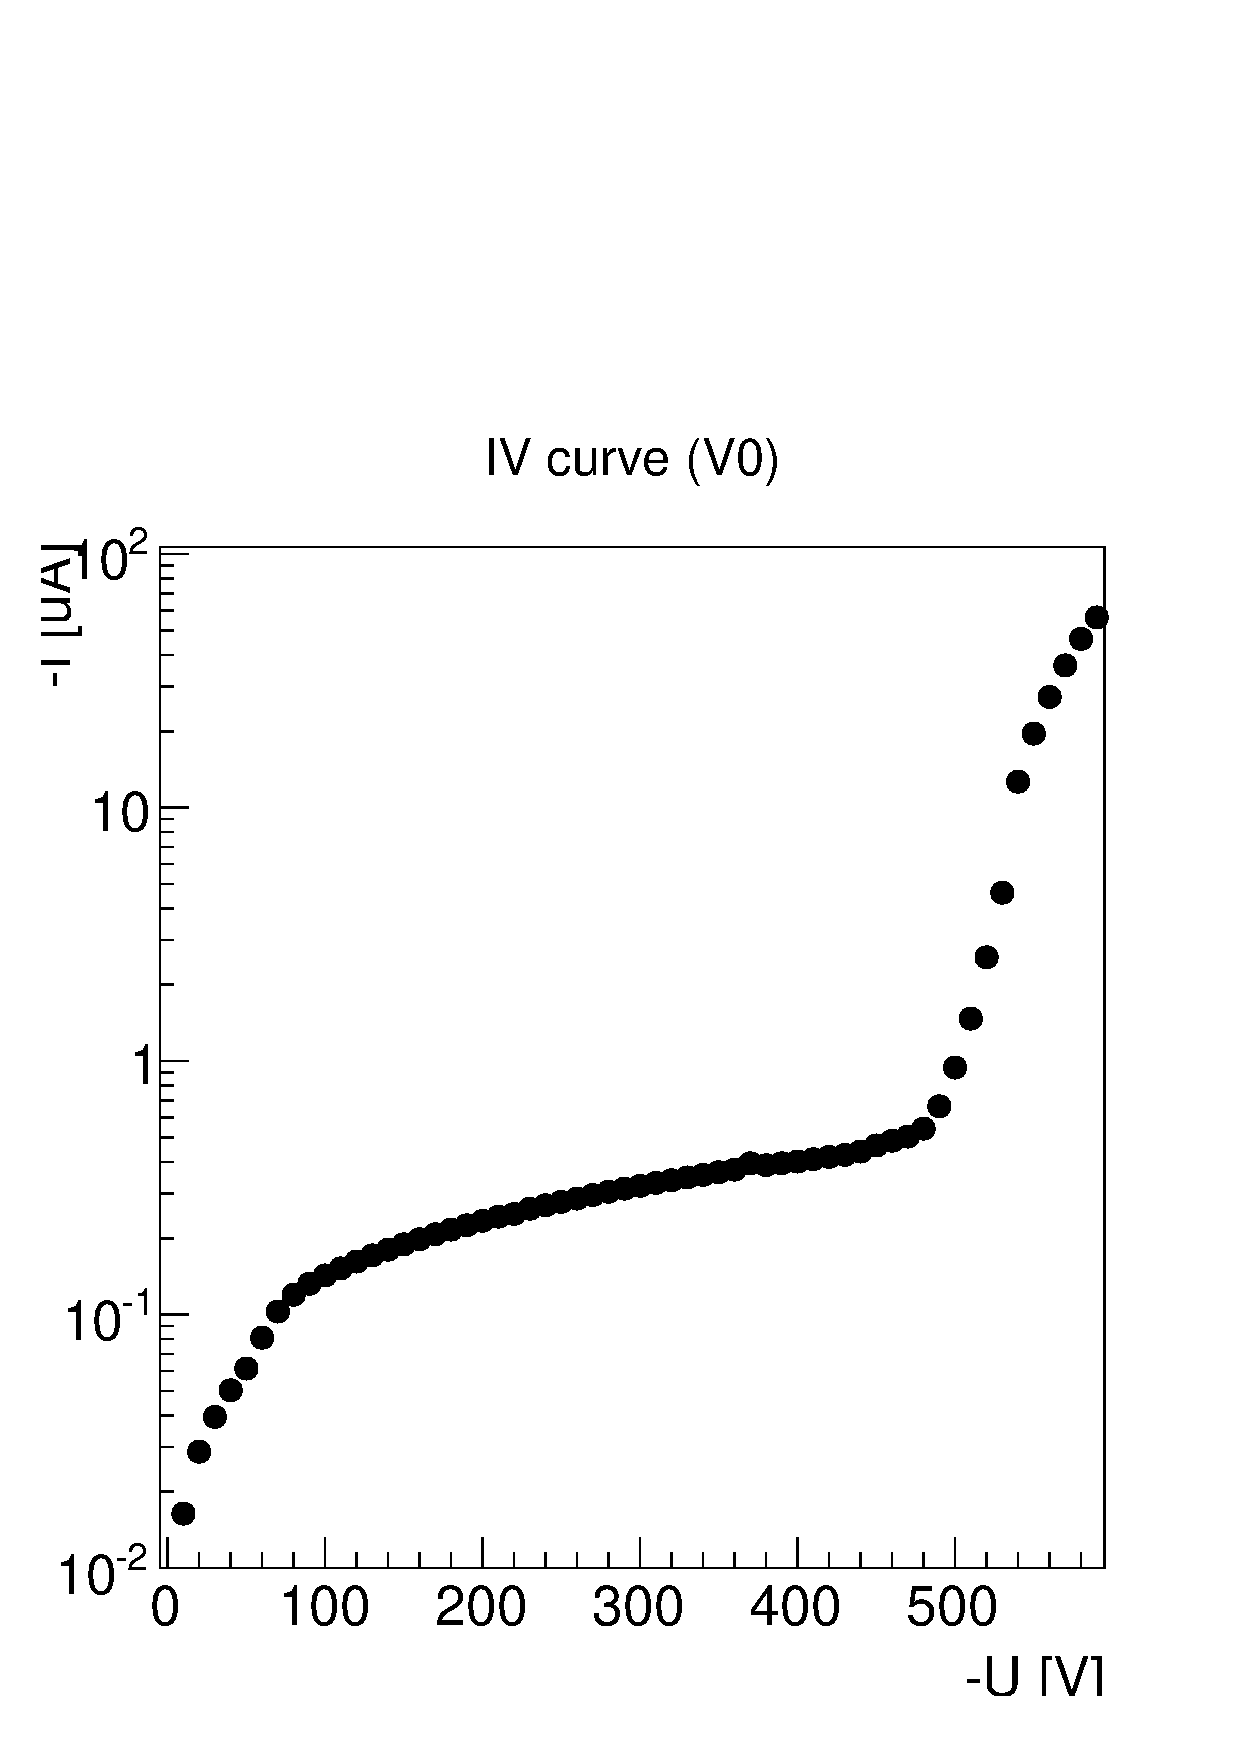
\includegraphics[width=0.4\textwidth]{ch7/iv_test}
  \caption[IV results of a module]{IV test for a fully assembly module.}\label{fig:iv_test}
\end{figure}

\subsubsection{Pretest}
It is composed of several subtests and its purpose is to check the basic functionalities of the ROCs and to calibrate some of the DAC {\rojo{list of DACs here or in ch 2}} settings. A couple of these subtests are: The \ital{ProgramRoc} measures the difference in current (Iana) drawn by the amplifiers when a voltage (Vana) is applied and remove. 
If the difference between these two measurements is non-zero it implies that we are able to change DAC values by sending a command, the ROC is programmable. This test is done for all 16 modules in a ROC. The \ital{SetVthrCompCalDel} subtest is done to optimize the value of the VthrComp and CalDel DACs. It chooses a pixel from within a ROC and sends 5 calibration pulses to PUC of this pixel. This process is repeated for the 256 x 256 parameter space of these DACs and the response of the pixel is read to make an efficiency plot. Then VthrComp is set to the lower plateau plus 50 units and CalDel is set to half of the left and right edges. Figure \ref{fig:pretest} shows the output of these subtests for a sample module

\begin{figure}[!h]
  \centering
  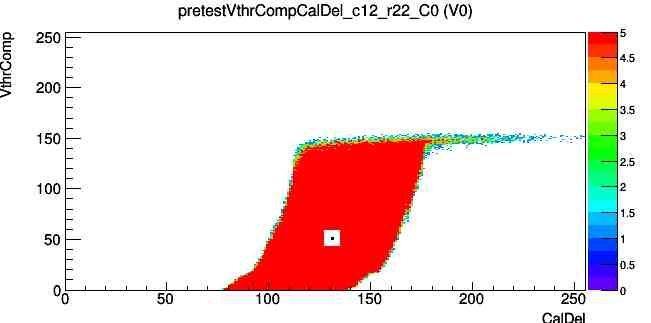
\includegraphics[width=0.7\textwidth]{../images/ch7/working_point}
  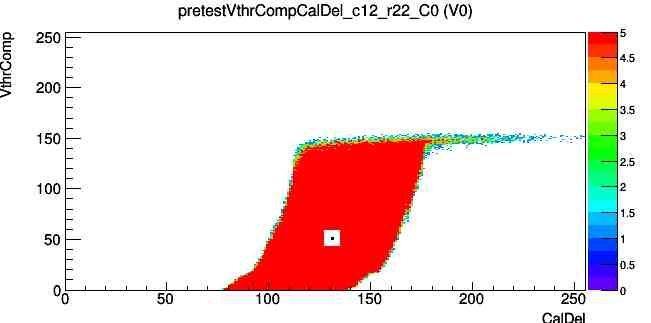
\includegraphics[width=0.7\textwidth]{../images/ch7/working_point}
  \caption[Programable ROC and working point]{Output of the ProgramRoc (left) and finding working pixel (right) subtests.}\label{fig:pretest}
\end{figure}

\subsubsection{Pixel Alive}
In the pixel alive test three subtests are performed: \ital{Alive test} checks for the response of a pixel by sending 10 calibration pulses (hits) to it and recording how many the pixel reports back. Pixel with 10 hits are marked as good, those with less than 10 hits are flagged as faulty, and those with zero hits are called dead. In the \ital{Mask test} all pixels are disable and the same efficiency measurement is done. Pixels with zero efficiency are marked as good while those with efficiency grater than zero are bad. The \ital{AddressDecoding} test checks the specific address of the pixel within the ROC. If the response of the pixel does not match the address to which it was sent the pixel if marked as bad. repeats the same procedure but checks that the order of the resulting data. If the address of a given pixel is out
of order, the recorded hit is given a negative pulse height value. Pixels with negative
hits are flagged as faulty. Figure \ref{fig:pix_ali} shows the result of the pixel alive test for a fully working module and Figure \ref{fig:pix_ali_bad} shows a module with faulty ROC and a ROC with faulty pixels. 

\begin{figure}[!h]
  \centering
   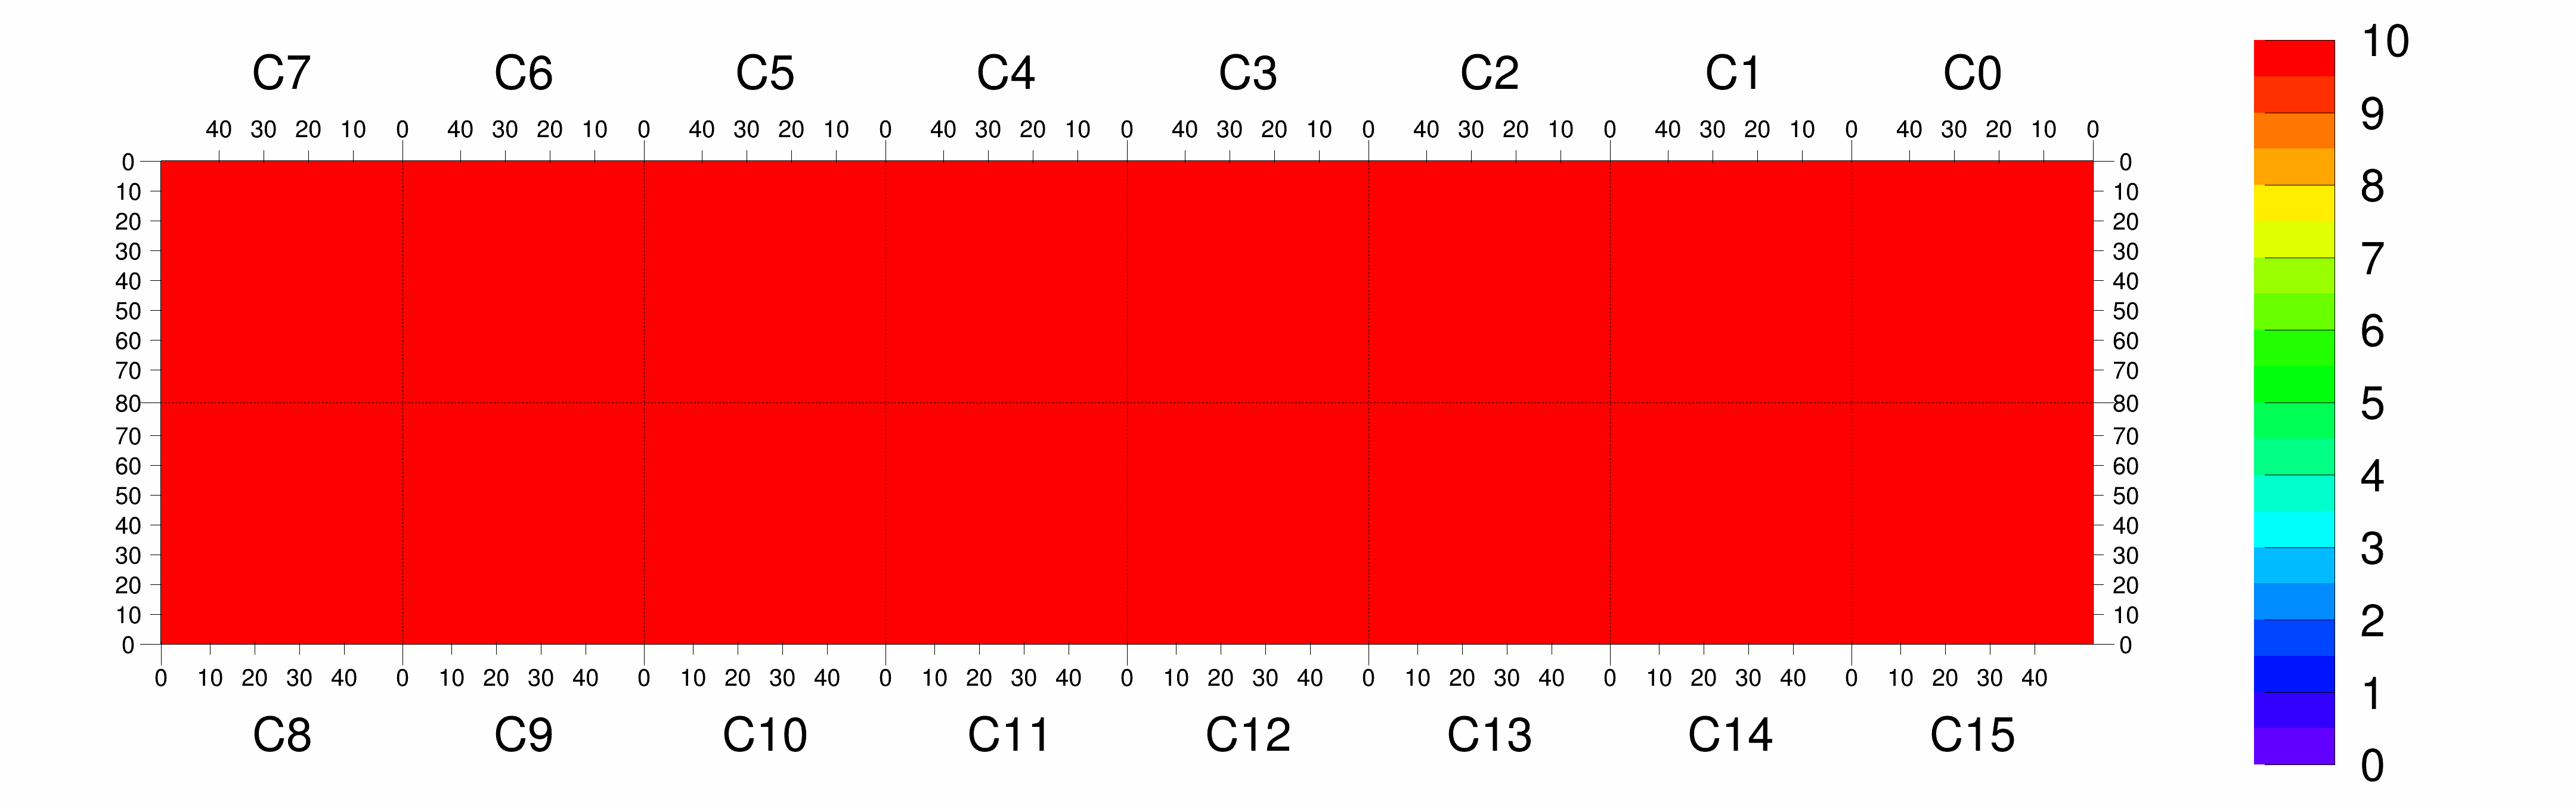
\includegraphics[width=0.3\textwidth]{ch7/pix_ali_good}
   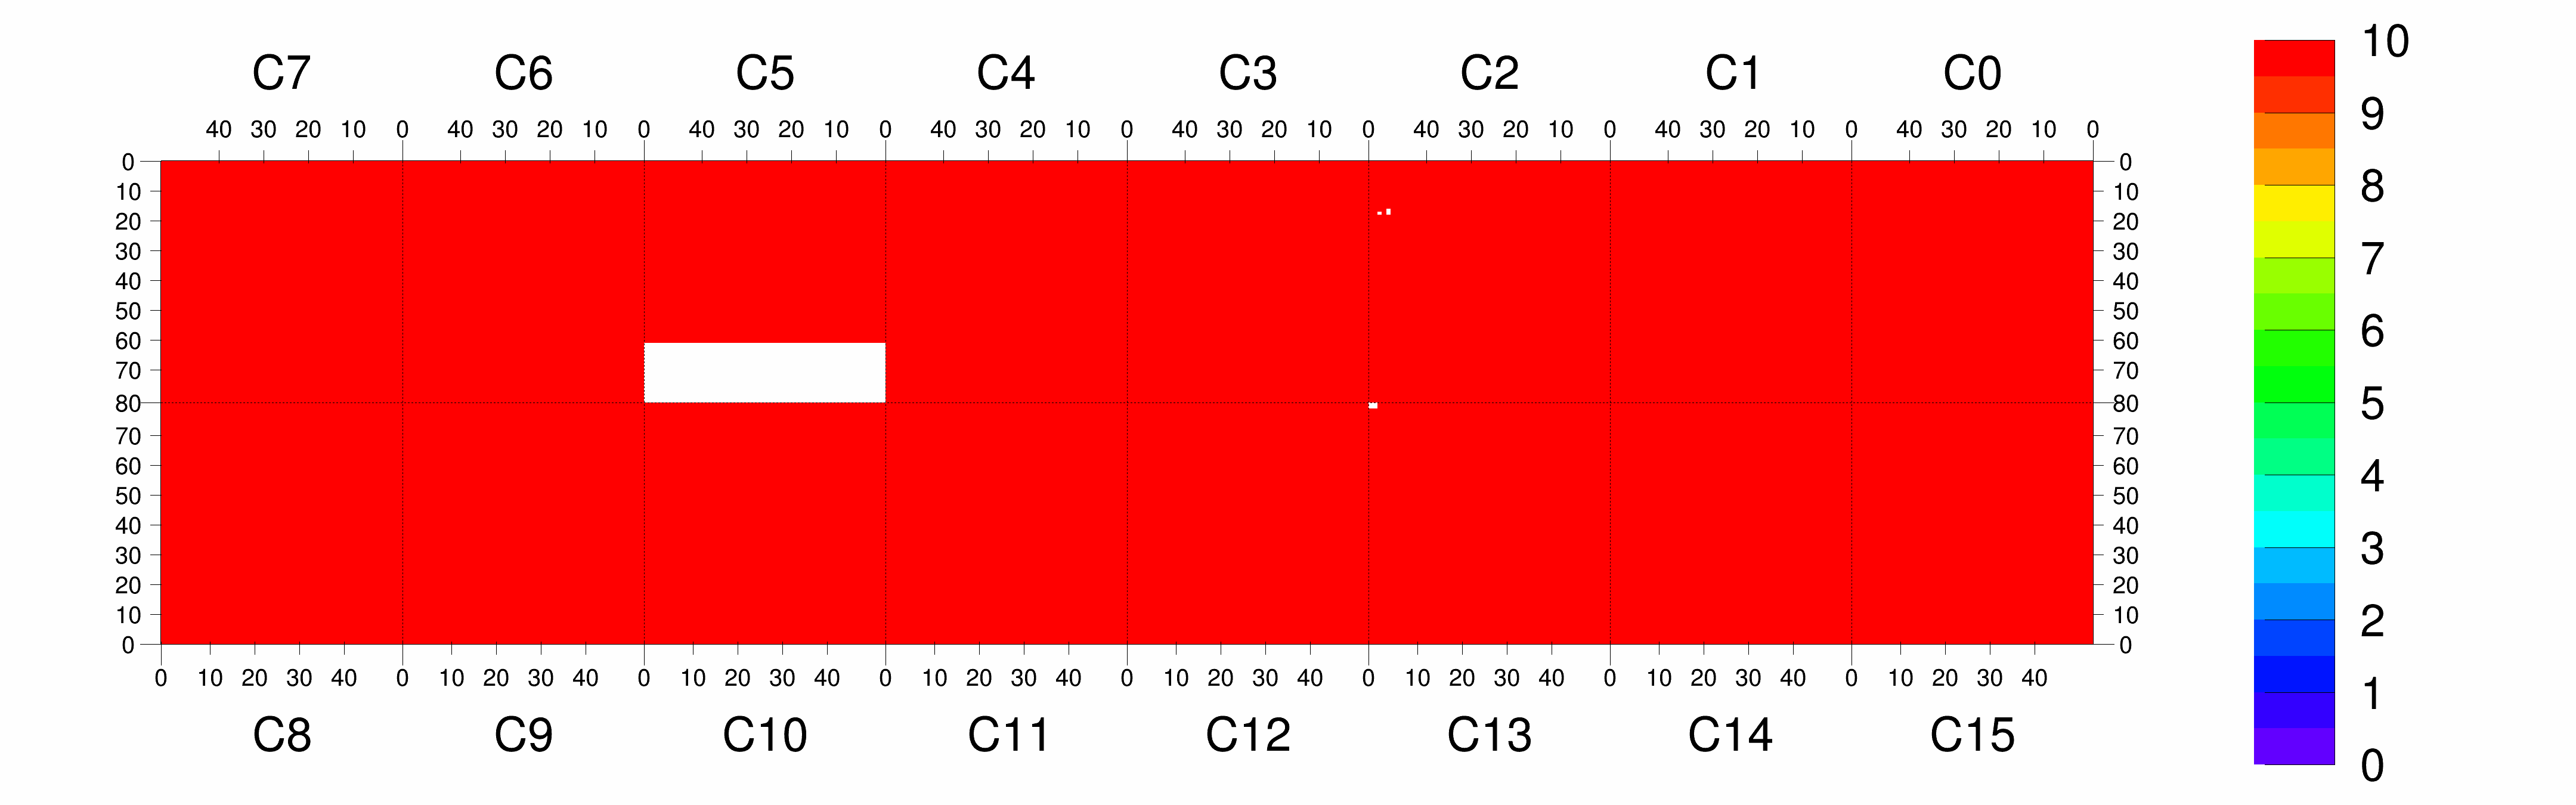
\includegraphics[width=0.3\textwidth]{ch7/pix_ali_bad}
   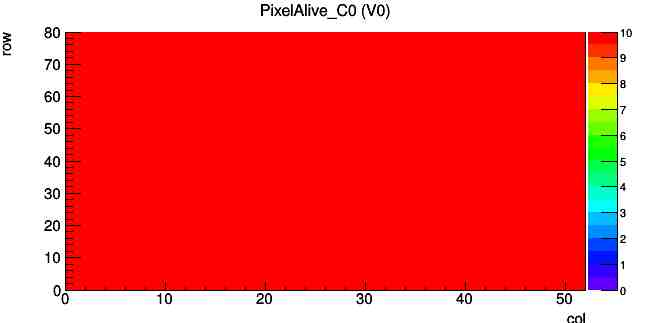
\includegraphics[width=0.3\textwidth]{ch7/pix_ali_full}
  \caption[Pixel alive test]{Pixel alive test for a fully assembled module. a) Alive test, b) Mask test, and c) AddressDecoding test.{\rojo{right fig}}}\label{fig:pix_ali}
\end{figure}

\begin{figure}[!h]
  \centering
   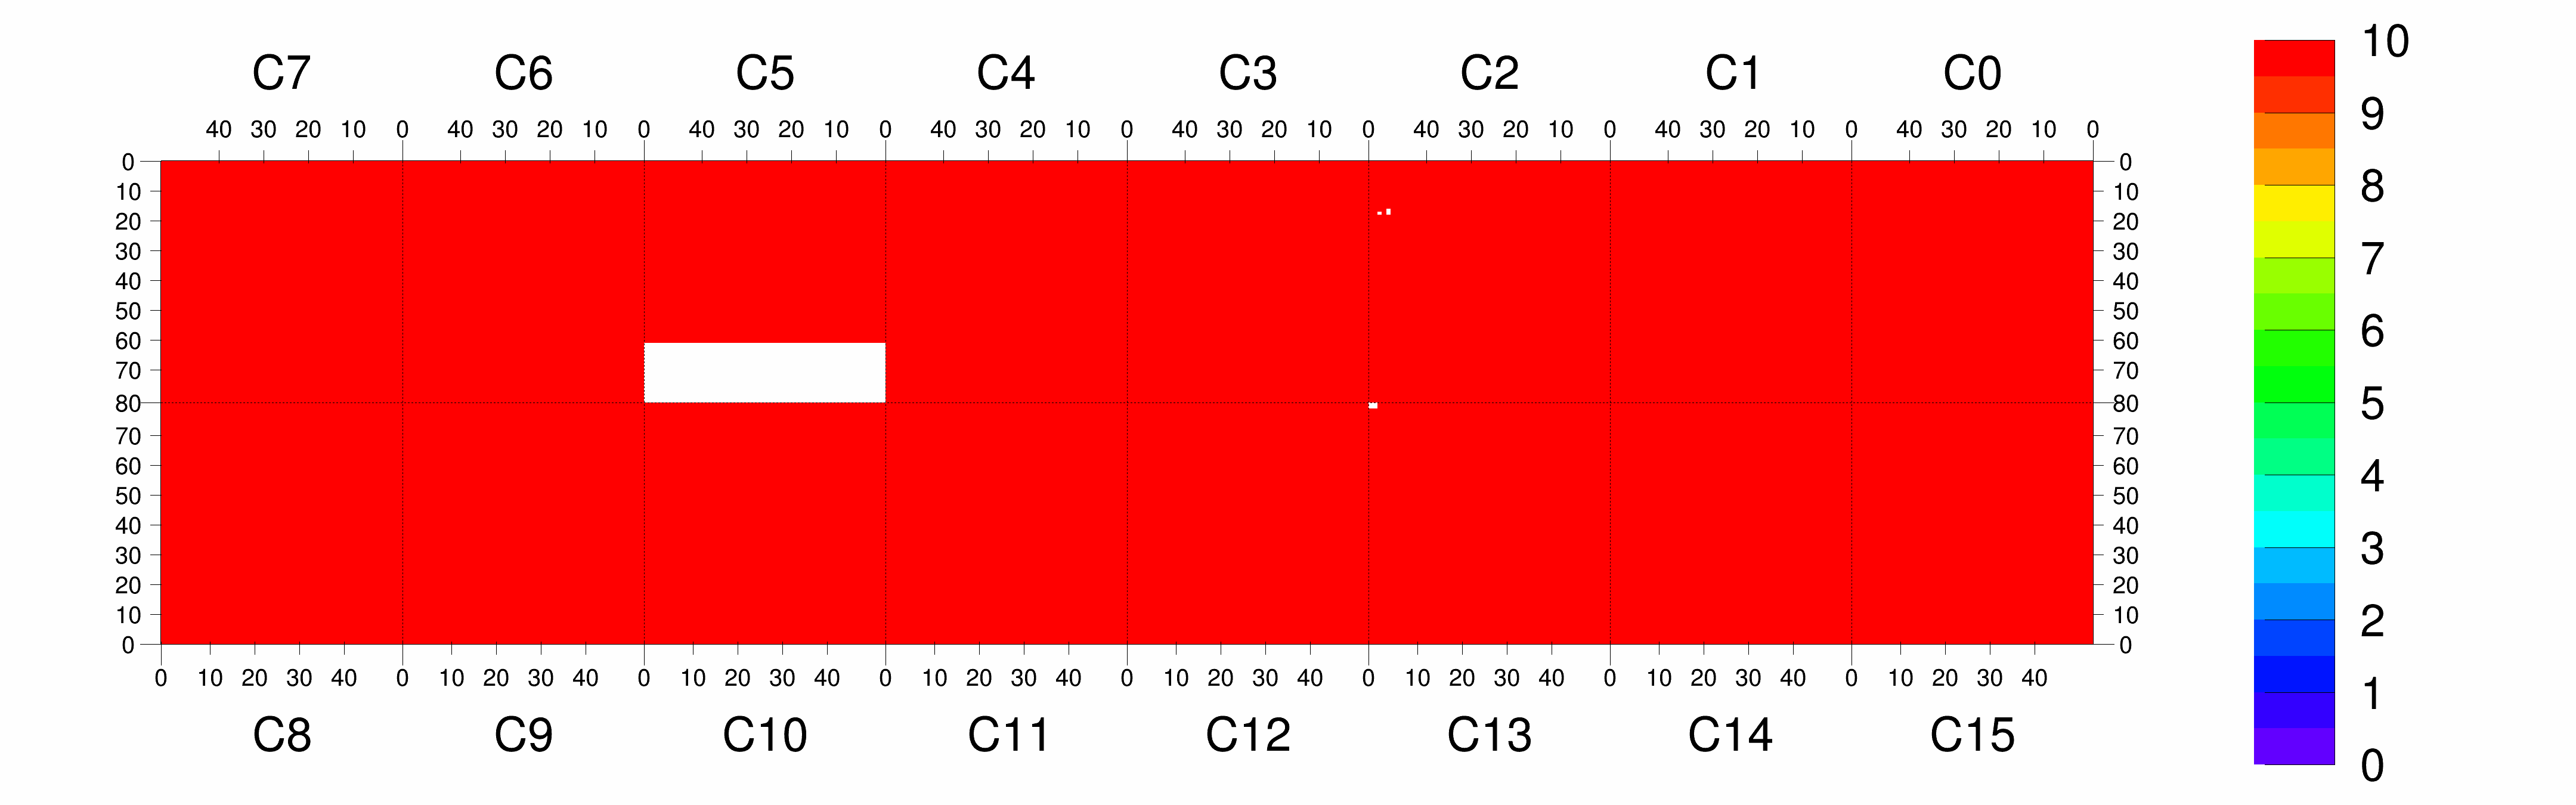
\includegraphics[width=0.4\textwidth]{ch7/pix_ali_bad}
   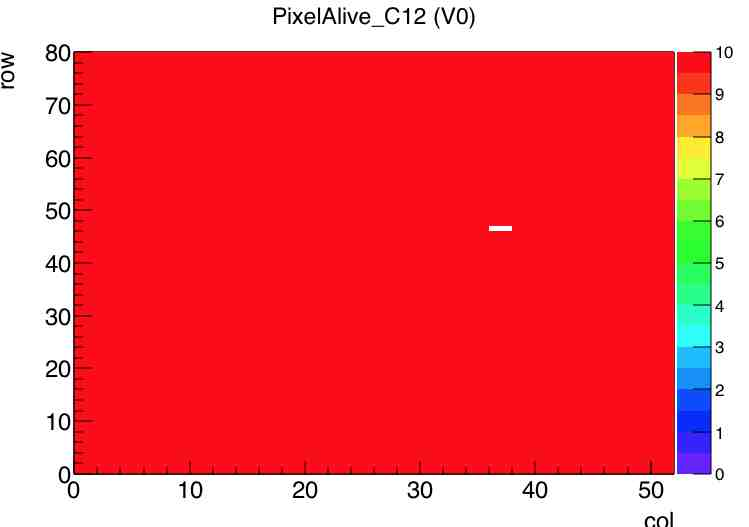
\includegraphics[width=0.3\textwidth]{ch7/pix_ali_roc}
  \caption[Faulty pixel alive test]{Pixel alive for a fully assembled module. a) a module with a faulty ROC and b) a ROC with faulty/dead pixels}\label{fig:pix_ali_bad}
\end{figure}

\subsubsection{Trimming Test}
The aim of the the trimming test is to (calibrate) set the threshold of all pixel on a ROC as uniform as possible. It attempts to do this by varying the VthrComp, Vtrim, and Trim bits DACs. The Trimming test sets VthrComp and Vtrim for the entire ROC and then uses trim bits to further refined the threshold of individual pixels. After the trimming test is finished all pixels within the ROC {\rojo{will have a threshold value as low as possible but still higher than the electrical noise.}}  Furthermore, a TrimBits subtest verifies that all trim bits are working by sequentially enabling each bit and observing its effect on the pixel threshold distribution. The trimming test works as follows: first, with Vcal set to a target value, it finds the VthrComp turn-on value by producing S-Curves for all pixels with respect to VthrComp. Then, VthrComp is set to the value of the pixel with the lowest turn-on value. A ROC map distribution of turn on values for a ROC can be seen in figure \ref{fig:turn-on}. Then, with the VthrComp set to its lowest value, the test tries to minimize the Vtrim value by repeating the previous process and finding the pixel with the highest Vcal turn-on value, see Fig \ref{fig:turn-on}. This is the pixel that requires the most trimming to have its Vcal threshold reduced to the target value. Following, with all trim bits enabled, the test performs an efficiency scan over Vtrim and Vcal DACs \ref{fig:turn-on} to find the value of Vtrim that corresponds to a turn-on at the target Vcal.

\begin{figure}[!h]
  \centering
  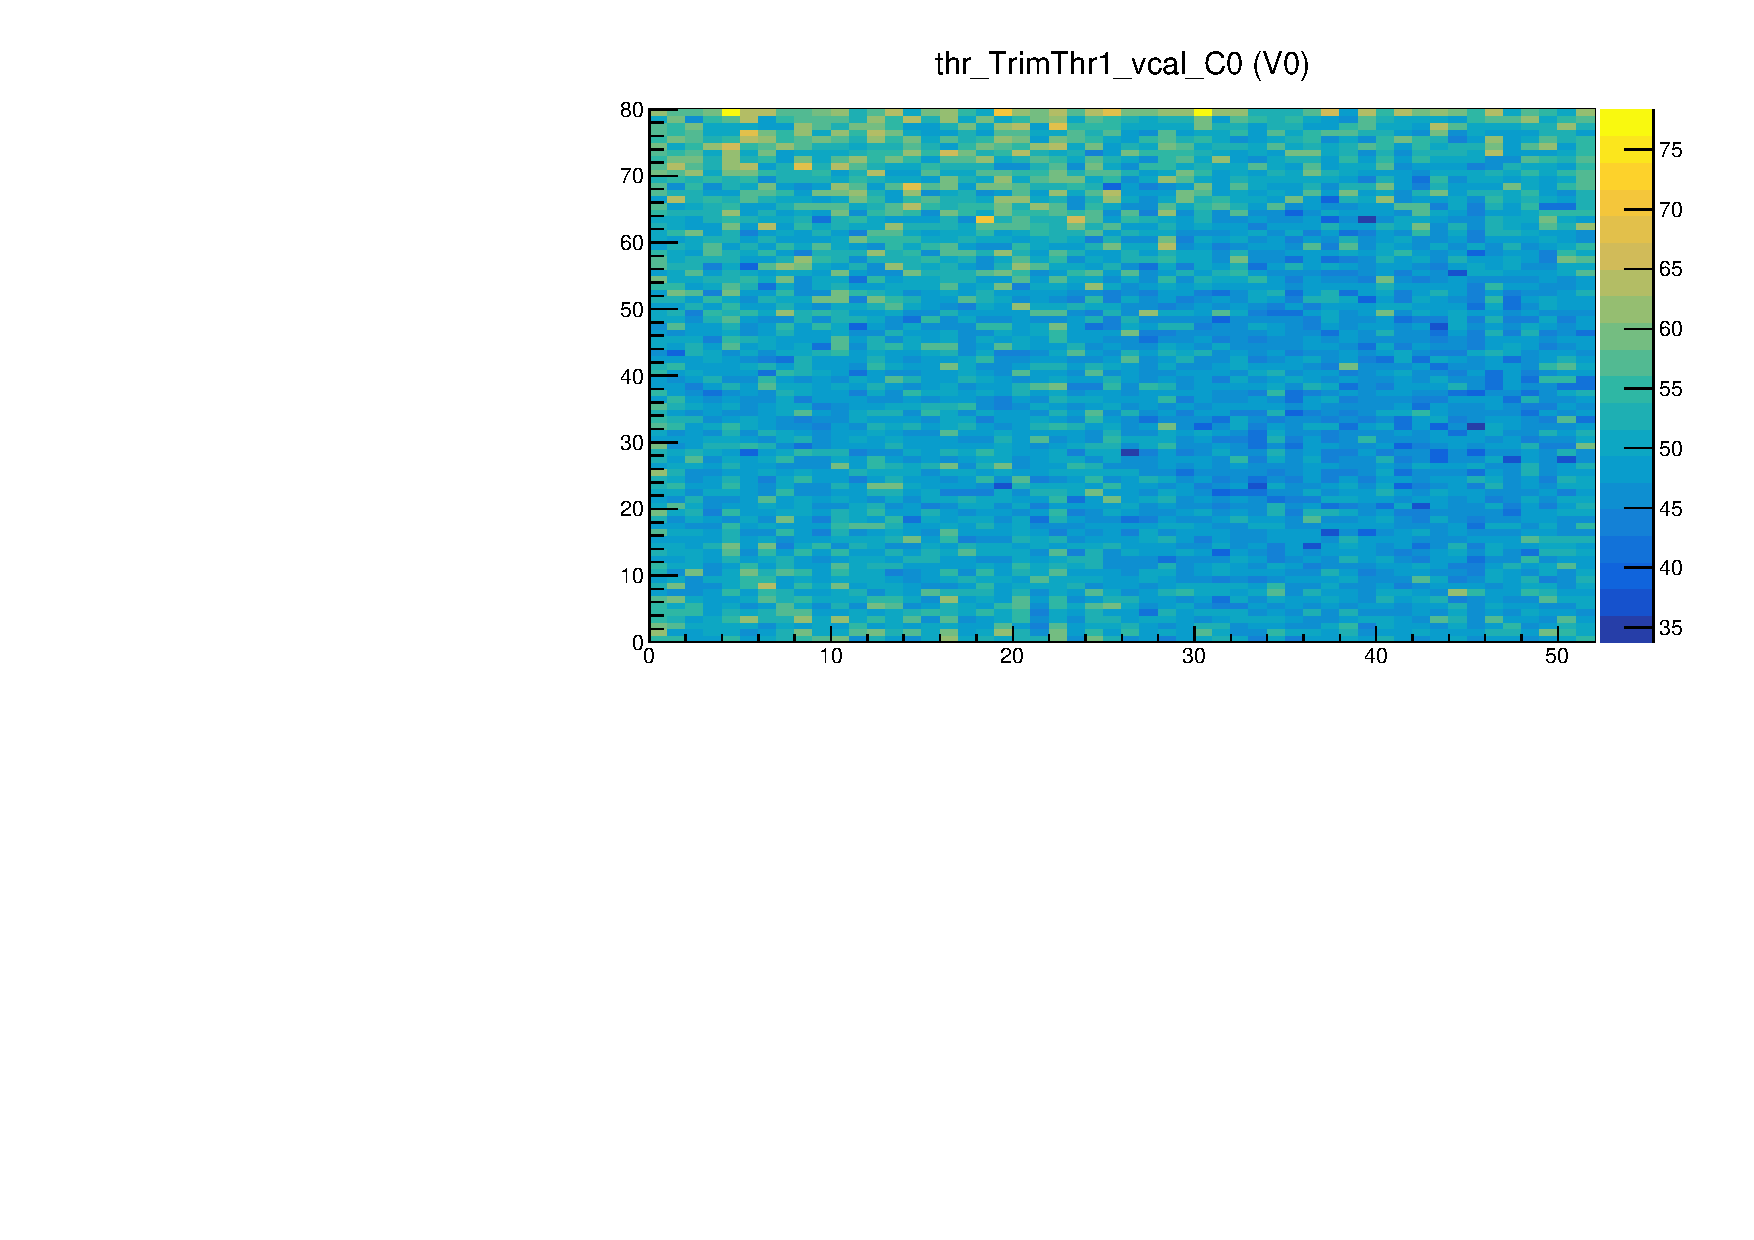
\includegraphics[width=0.3\textwidth]{/ch7/trim_turn-on_vcal}
  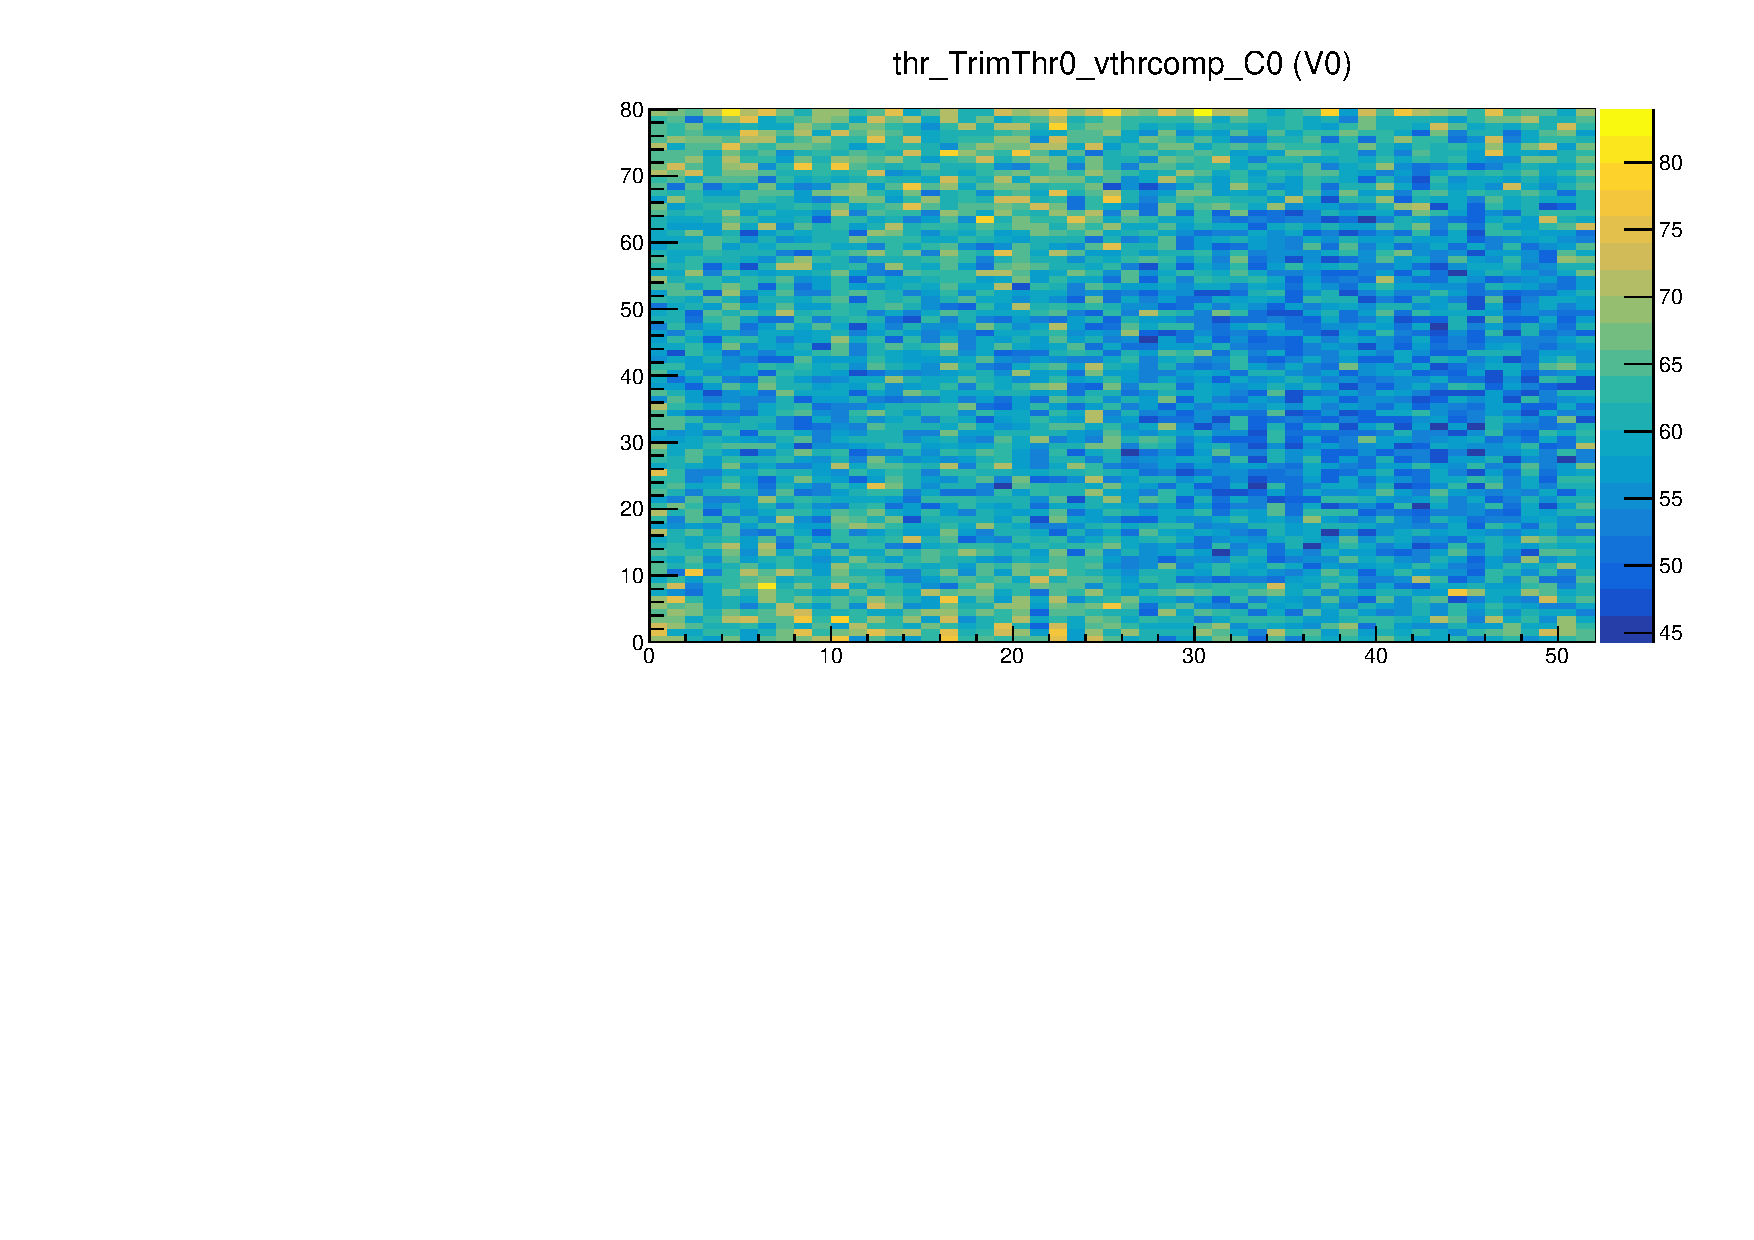
\includegraphics[width=0.4\textwidth]{/ch7/trim_turn-on_vthr}
  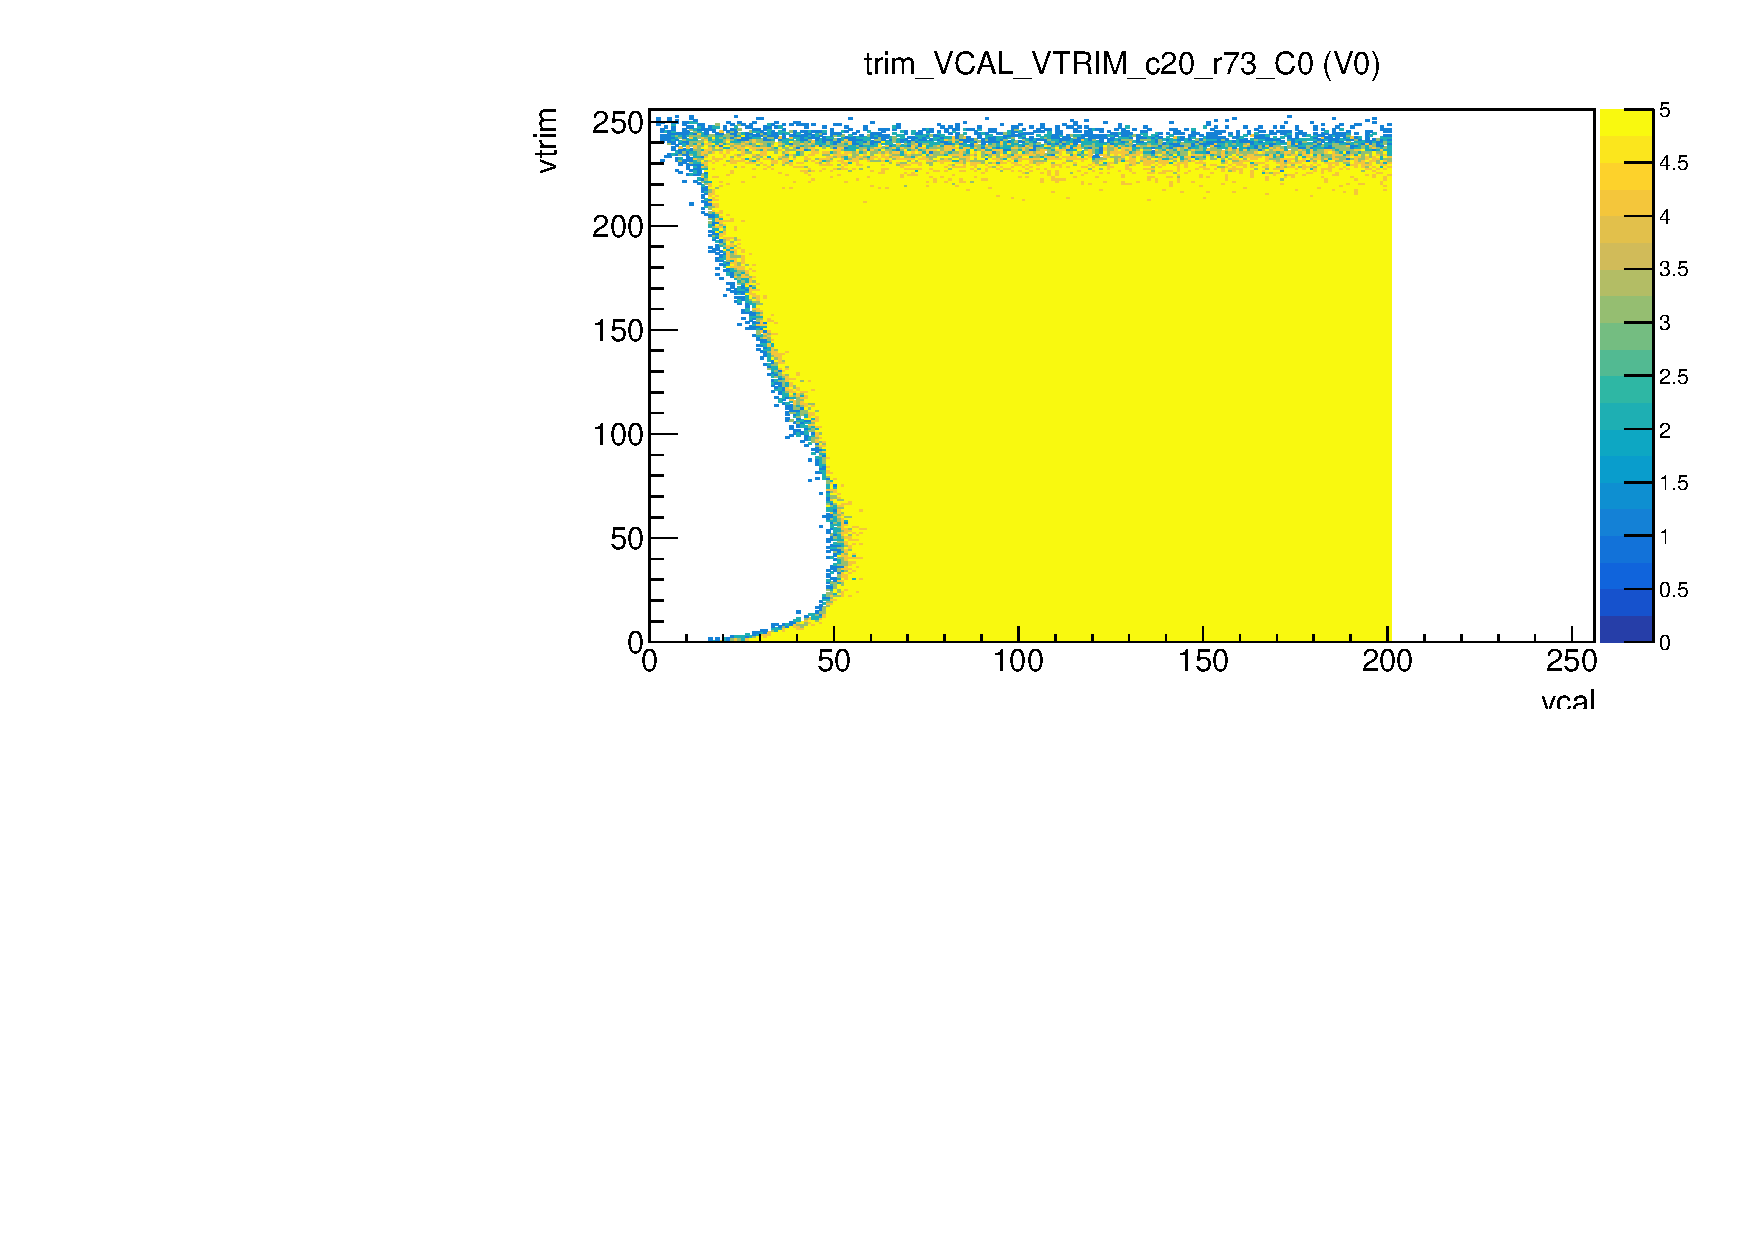
\includegraphics[width=0.3\textwidth]{/ch7/trim_eff}
  \caption[Trim test turn on]{Trim test optimization for. left: Vcal turn on, center: Vthr turn on, right: efficiency in the Vtrim-Vcal plane.}\label{fig:turn-on}
\end{figure}

Next, starting from a high Vtrim, its value is iteratively lowered until the Vcal turn-on surpasses the target Vcal, which corresponds to the minimum value that can trim this pixel. This is the final value of the Vtrim DAC for the the ROC. Finally, with the values of the VthrCaomp and Vtrim set, the test refine the threshold on each pixel by modifying the 4 Trim bits. Starting with the Trim bits set to 7 [0111],    scurves are used to find the Vcal turn-on value. If the pixel {\rojo{reports a hit}} fires below (above) the target Vcal value, the Trim bits value is increased (decreased) by 4, so that the amount of trimming is decreased (increased). This process is repeated three more time increasing or decreasing the Trim bits values by 2, 1, and 1 unit respectively, covering the full range, 0-15, of the Trim bits. Figure \ref{fig:trim_bits} shows a ROC map of Vcal for Trim bits = 7 and after 4 corrections are made and the final Vcal map and distribution could be seen in figure \ref{fig:trim_final}. 

\begin{figure}[!h]
  \centering
  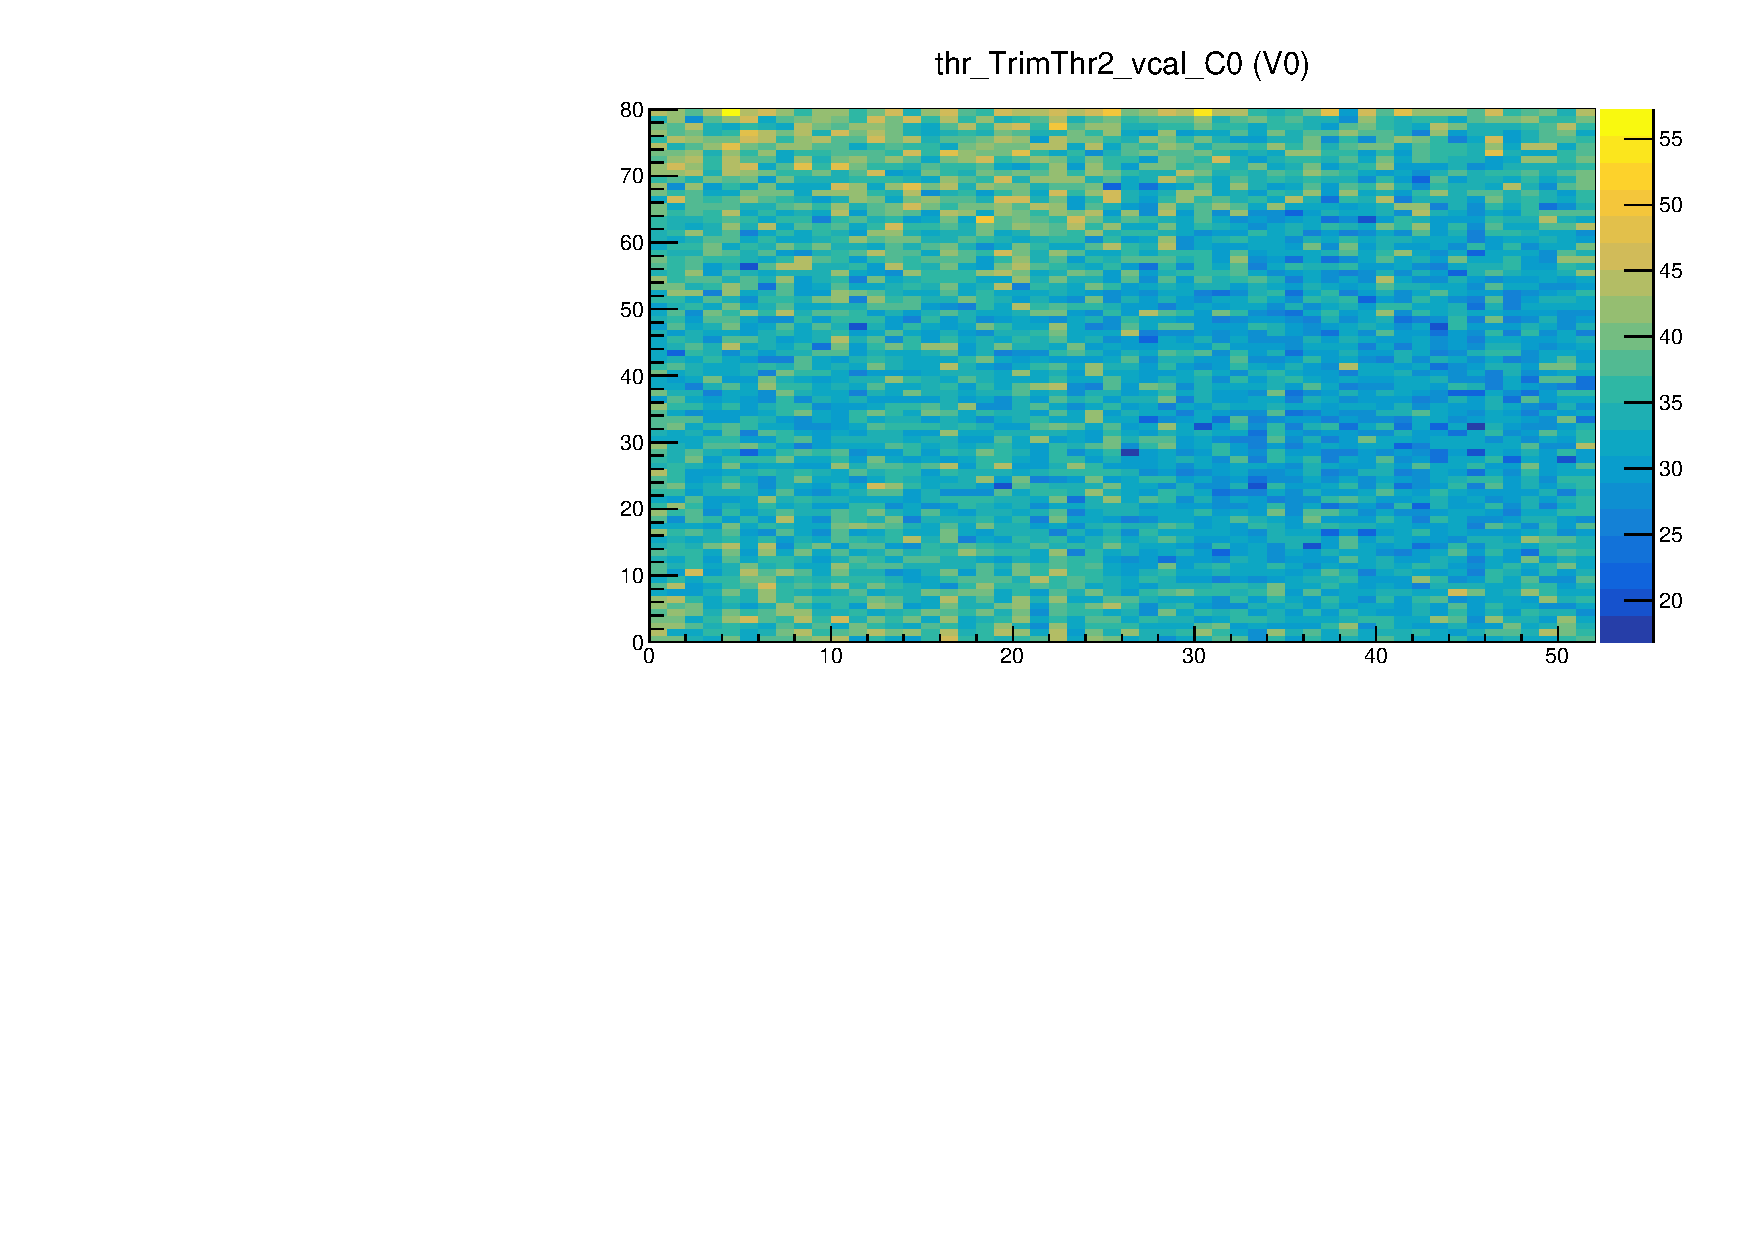
\includegraphics[width=0.7\textwidth]{/ch7/trim_bits_7}
  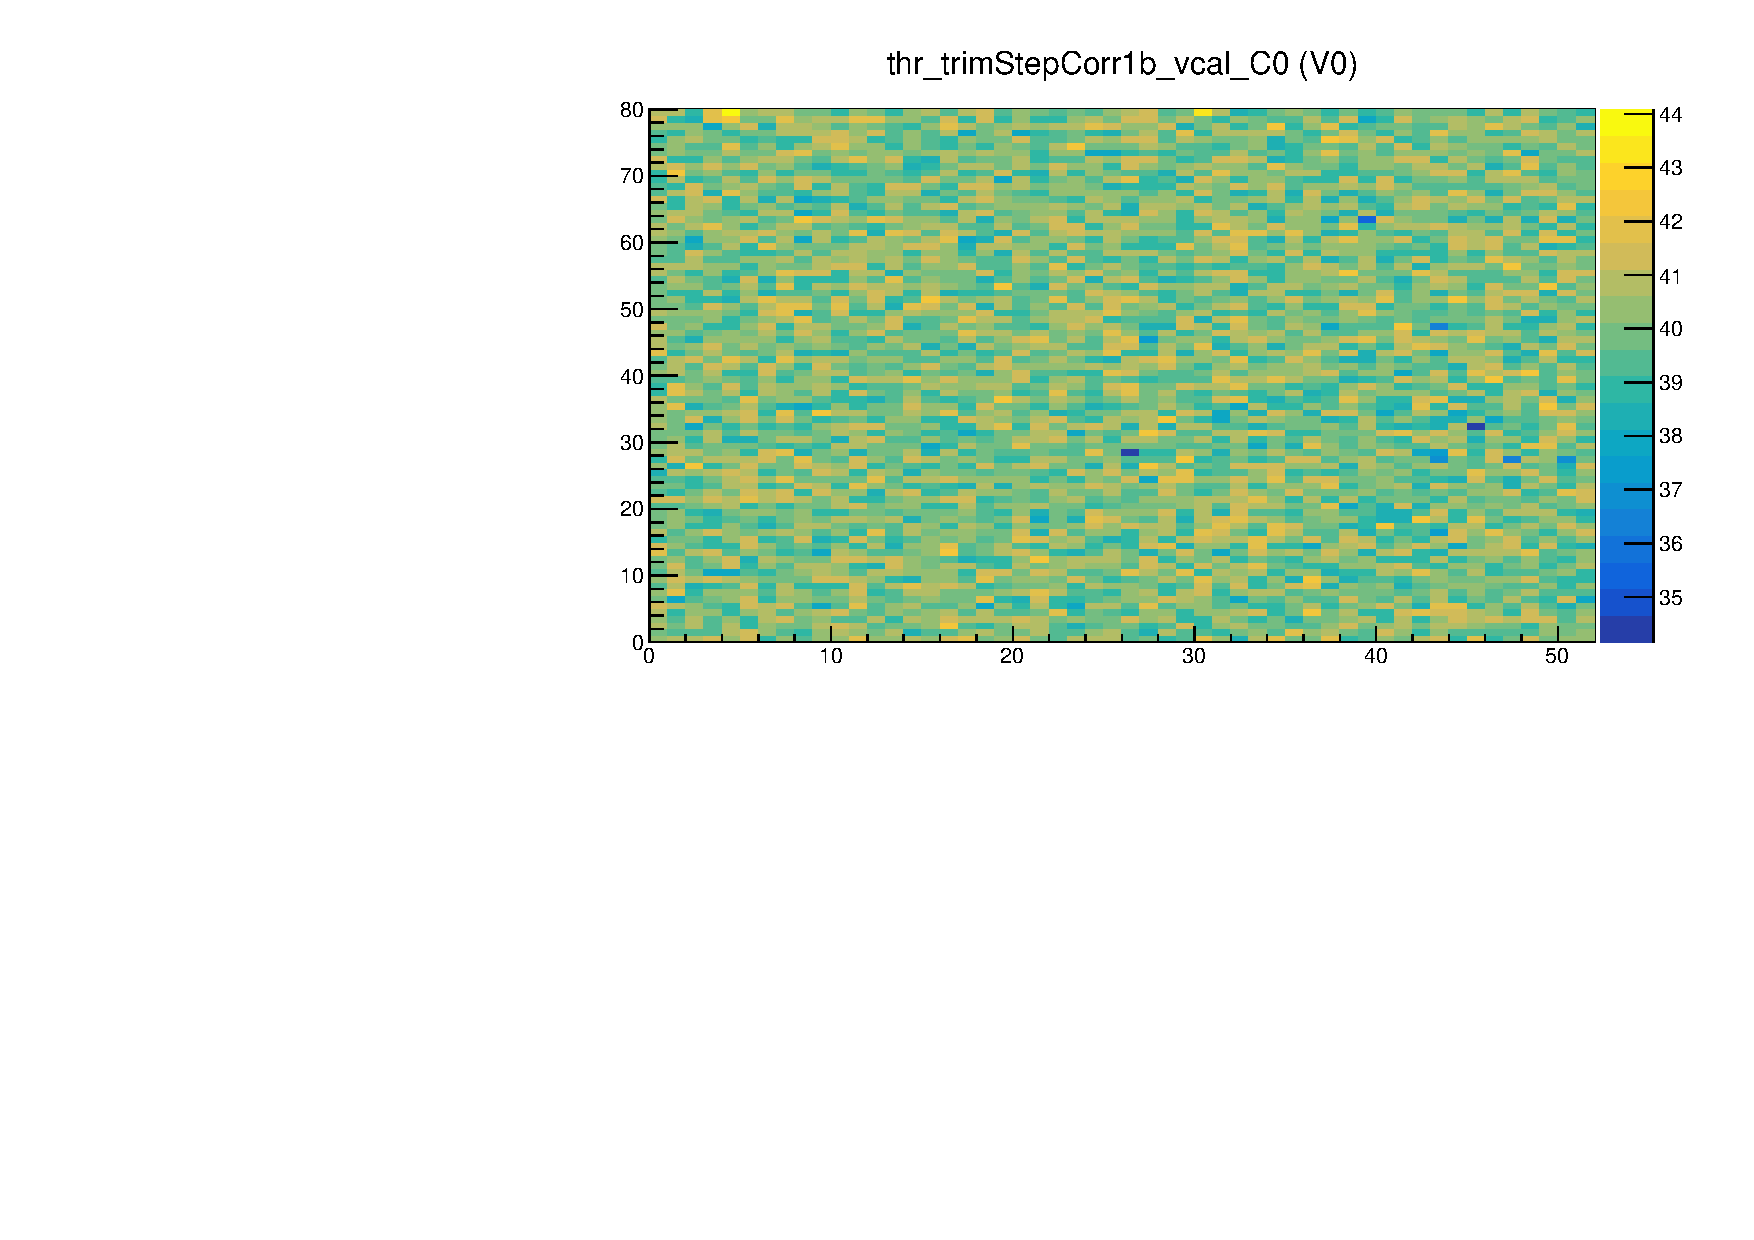
\includegraphics[width=0.7\textwidth]{/ch7/trim_bits_corr}
  \caption[Trim test Trim bits]{Trim bits map distributions for the Vcal turn-on values for the initial  and final Trim bits values.}\label{fig:trim_bits}
\end{figure}

\begin{figure}[!h]
  \centering
  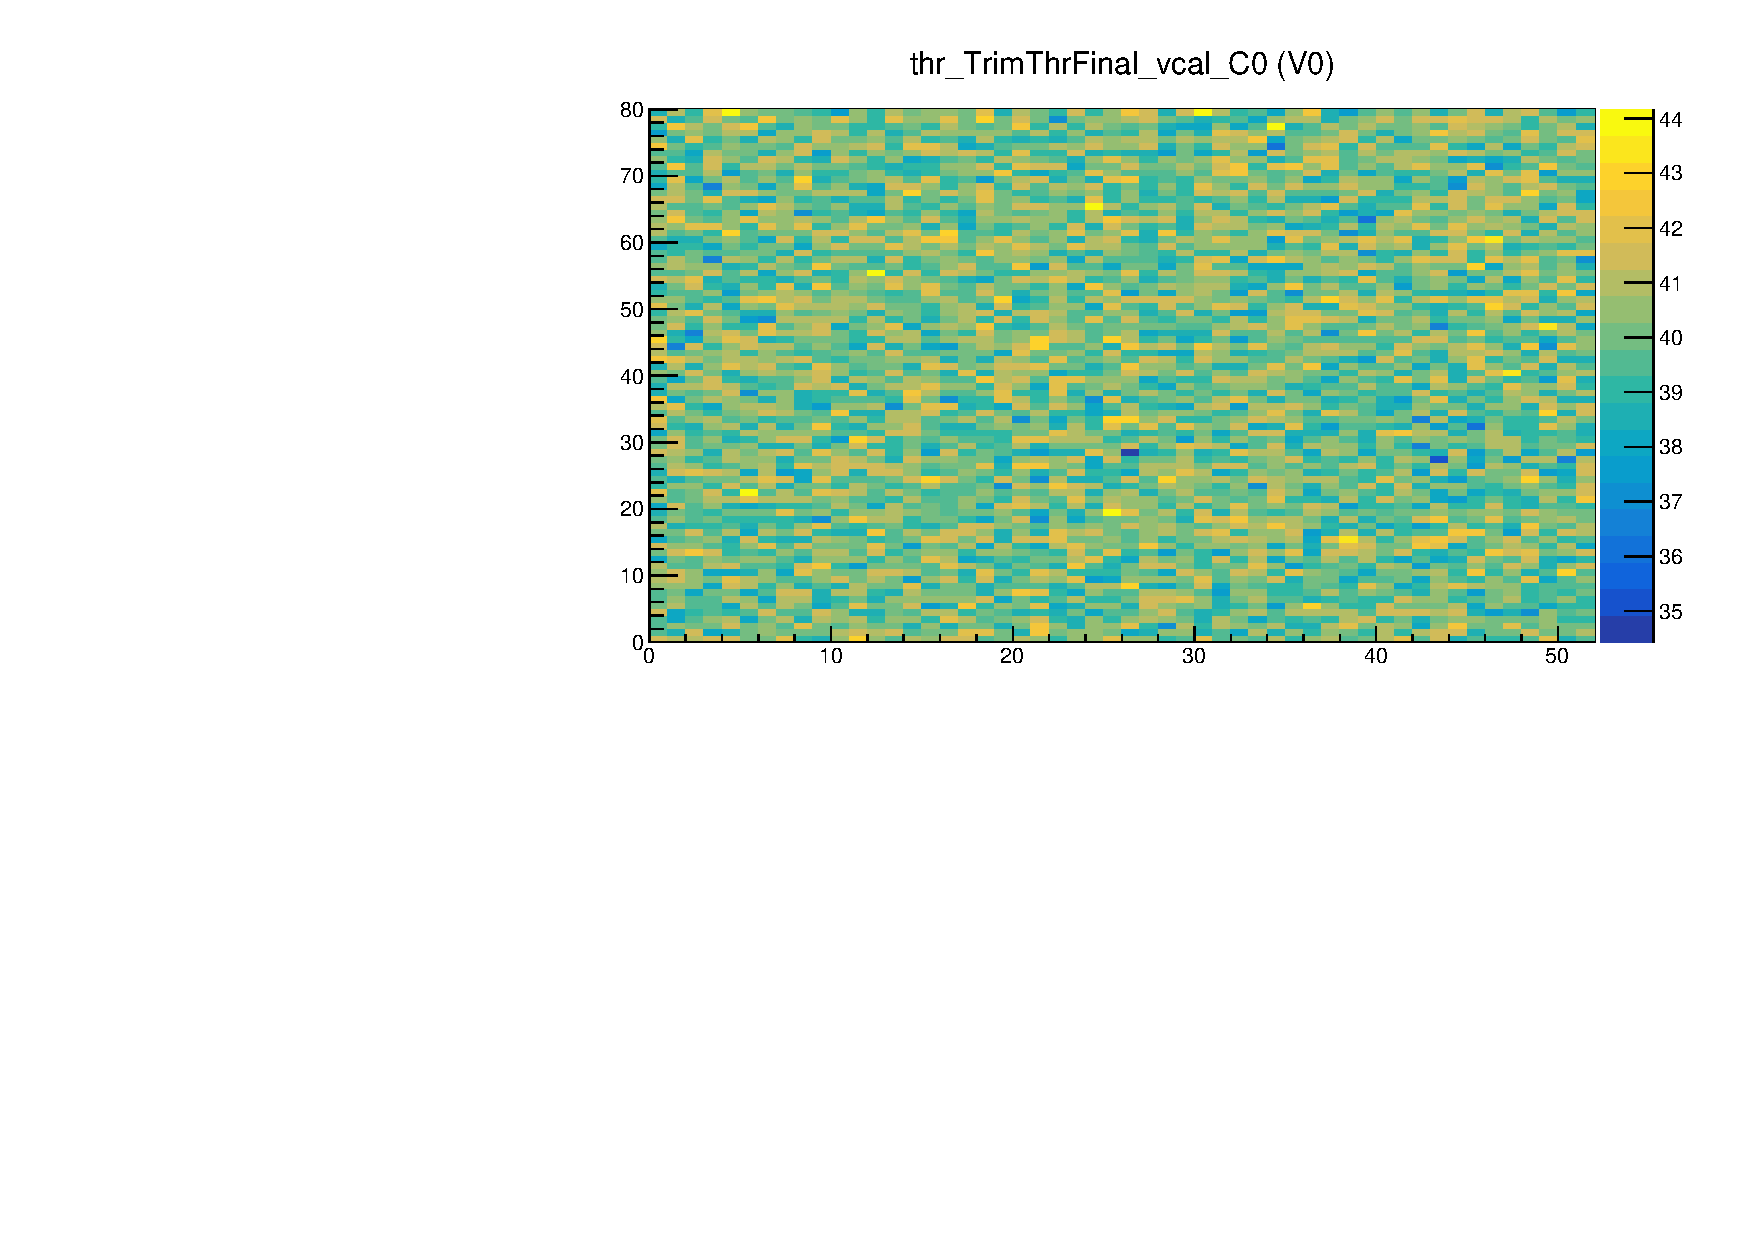
\includegraphics[width=0.7\textwidth]{/ch7/trim_final_map}
  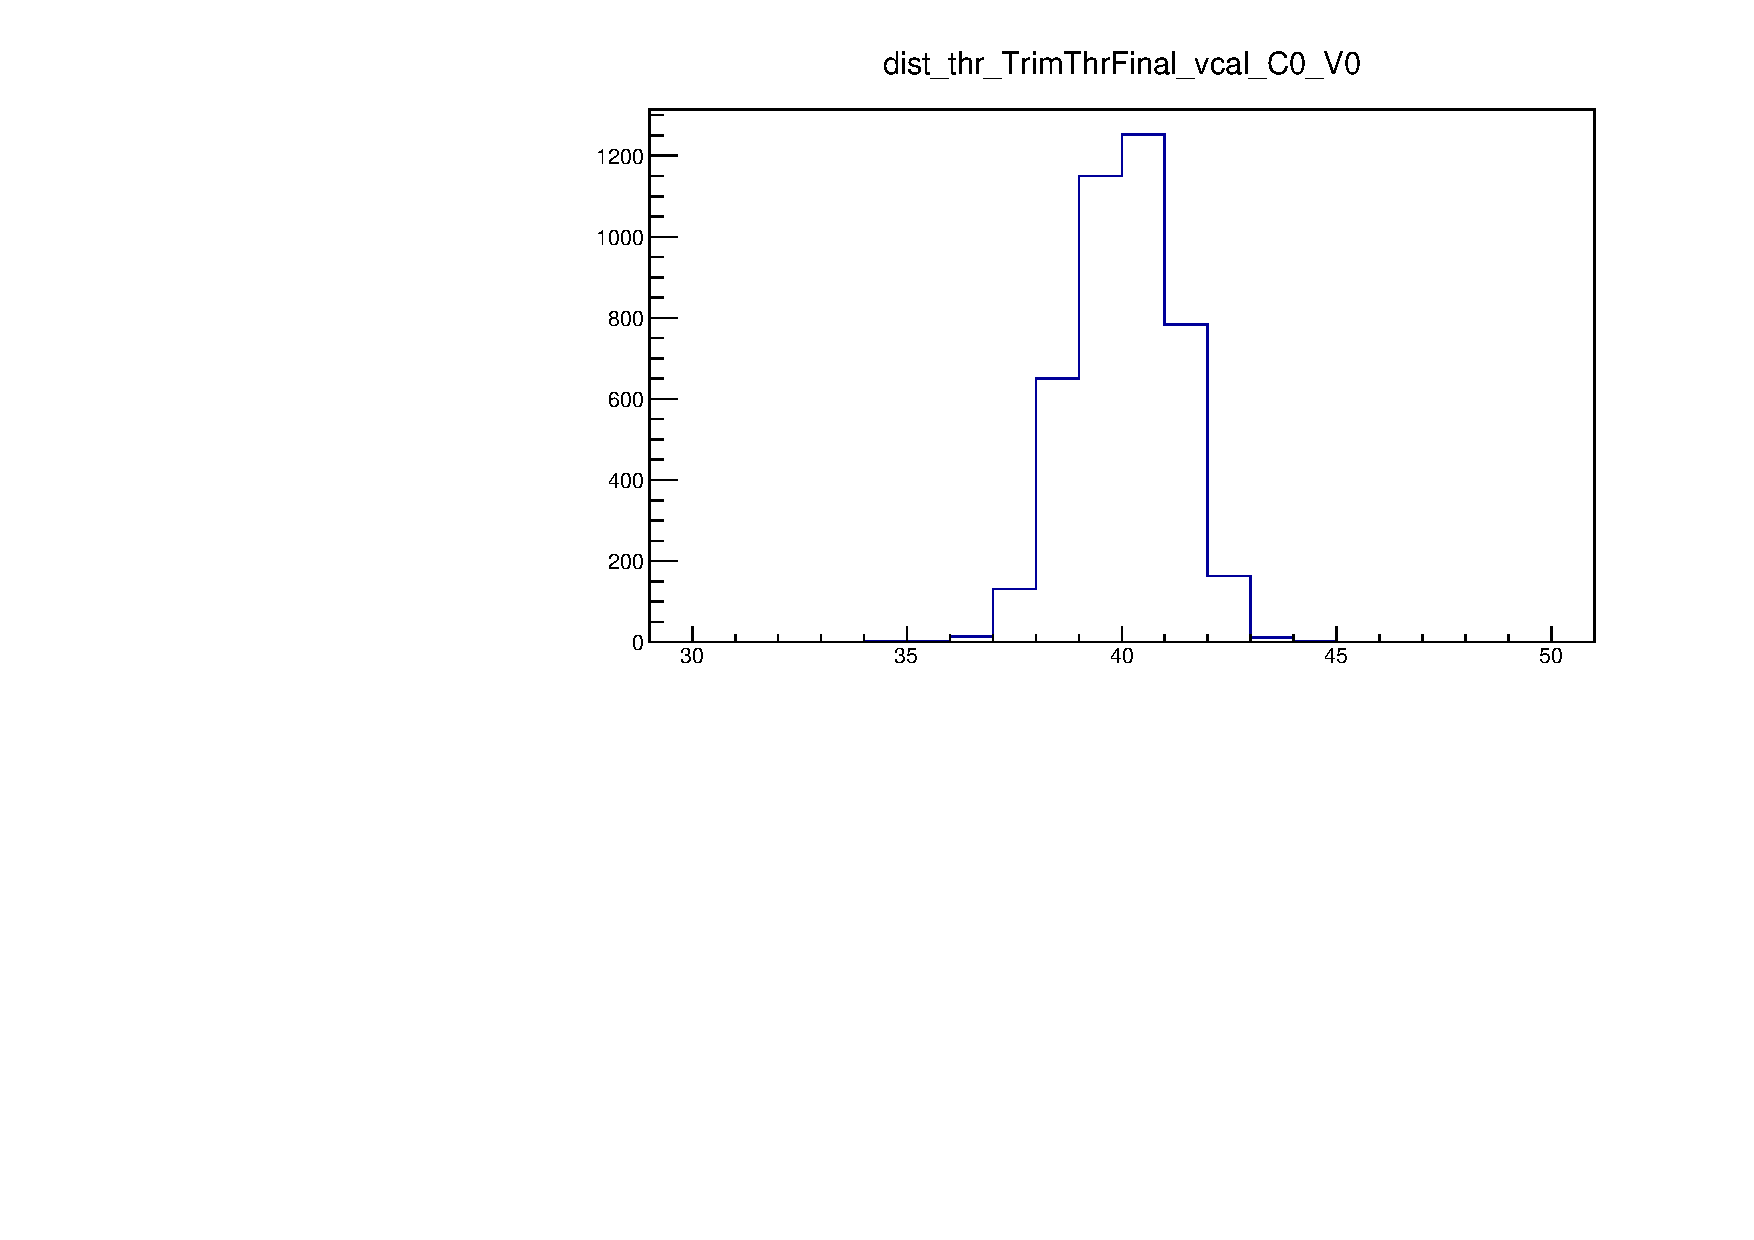
\includegraphics[width=0.7\textwidth]{/ch7/trim_final_dist}
  \caption[Trim test final]{Final map and distribution of Vcal threshold after the Trim test have finished.}\label{fig:trim_final}
\end{figure}

\subsubsection{PH Optimization}


%The PHOptimization test is responsible for setting an appropriate dynamic range for the 8-bit ADC that digitizes the recorded pulse height. The ADC is located in the Controller and Interface Block of the ROC. It can be seen in the bottom right box of Figure 1. The two DACs used to configure the ADC are PHOffset and PHScale. PHOffset adds a constant offset to the pulse height measurement, while PHScale effectively sets the gain of the ADC. The PHOptimization test is designed to optimize these DACs based on a highly sensitive and highly insensitive pixel in the given ROC, or, in other words, pixels with a very high and very low inherent gain. To use the ADC most effectively, the range of the ADC PH response as a function of Vcal needs to be optimized. On the low end, the ADC should provide a PH well above noise for the low-gain pixel near the lowest Vcal that registers a hit on it. On the high end, the ADC should saturate for the high-gain pixel at some user-defined Vcal well below the maximum Vcal the ROC can provide. This allows the signal strength required for saturation to be measured and 

%\begin{figure}[!h]
 % \centering
  %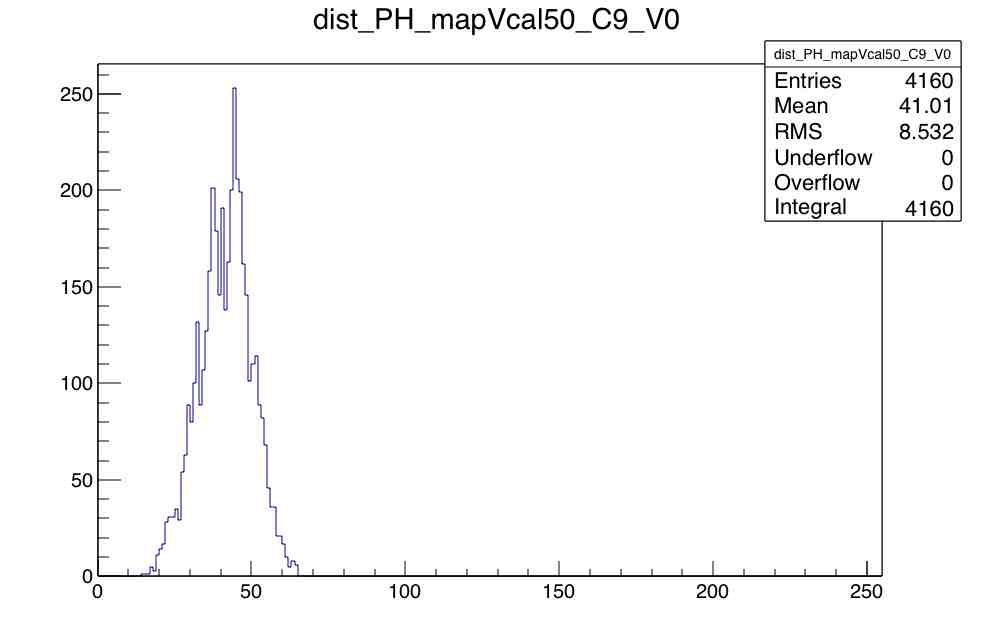
\includegraphics[width=0.7\textwidth]{../images/ch7/ph_opt}
  %\caption[Ph Optimization.]{PH optimization.}\label{fig:vis_insp}
%\end{figure}


\subsubsection{Gain Pedestal}
%The GainPedestal test does not alter any DAC parameters, but merely evaluates and records the shape of the pulse height vs. Vcal distribution for each pixel. For each pixel, this curve is fitted and the fit parameters are stored for later use. Since variations in gain are expected between pixels in a ROC, the gain must be measured independently for each pixel so that the pulse height to be calibrated back to the input signal size, in units of the Vcal DAC (low range). 4.5.2 Methodology For each pixel, a PH vs. Vcal curve is produced. To save time, the pulse height is sampled for a predetermined set of Vcal values instead of doing a complete Vcal scan. In the low Vcal range, the PH is measured in steps of 10 DAC units (configurable), from 10 to 255. Then, in the high Vcal range, the PH is measured for values of 30, 50, 70, 90, and 200. The results of these two scans are then combined into a PH vs. Vcal curve over the full Vcal range. This curve converts the high range Vcal values to their larger low range equivalents by multiplying by a factor of 7. This curve is then fit to an error function and the four fitted parameters and their errors are recorded. Parameter 0 corresponds to the Vcal value at the center of the error function, when the PH is halfway between zero and saturation (255). Parameter 1 is proportional to the width of the turn-on and is therefore inversely related to the gain of the pixel. Parameter 2 shifts the error function upwards, with a value of unity moving the floor of the function to zero. Parameter 3 corresponds to half the height of the function, and should be near 127.5 (255/2). The

%\begin{figure}[!h]
 % \centering
  %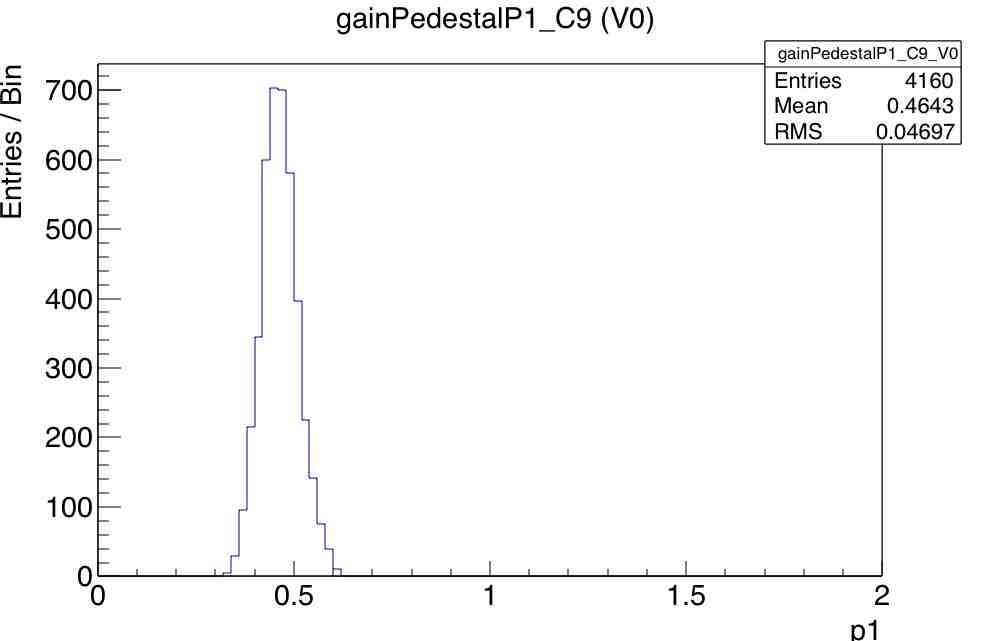
\includegraphics[width=0.7\textwidth]{../images/ch7/gain_ped}
%  \caption[Gain Pedestal.]{Gain pedestal.}\label{fig:vis_insp}
%\end{figure}

\subsubsection{Scurve Test}
The SCurve test measures the efficiency of a pixel as a function of Vcal. It is based on the assumption that a pixel will not respond to lower values of Vcal but it will always respond for higher values. In the absence of noise this curve will be just a step function which changes from zero effiecinecy below the threshold to a region of 100\% efficiency above. The effect of the noise is to smear out the step function giving it a \ital{S} shape. As the noise is assume to follow a Gaussian distribution, the SCurve if fitted with an error function and its width is a measure of the noise level in the pixel. Since the Vcal is known at this point in the testing procedure the SCurve is done around this Vcal value. In order to extract an accurate estimate of the width the number of triggers used for the test is 200. The output of this test can seen in figure \ref{fig:scurve}

\begin{figure}[!h]
  \centering
  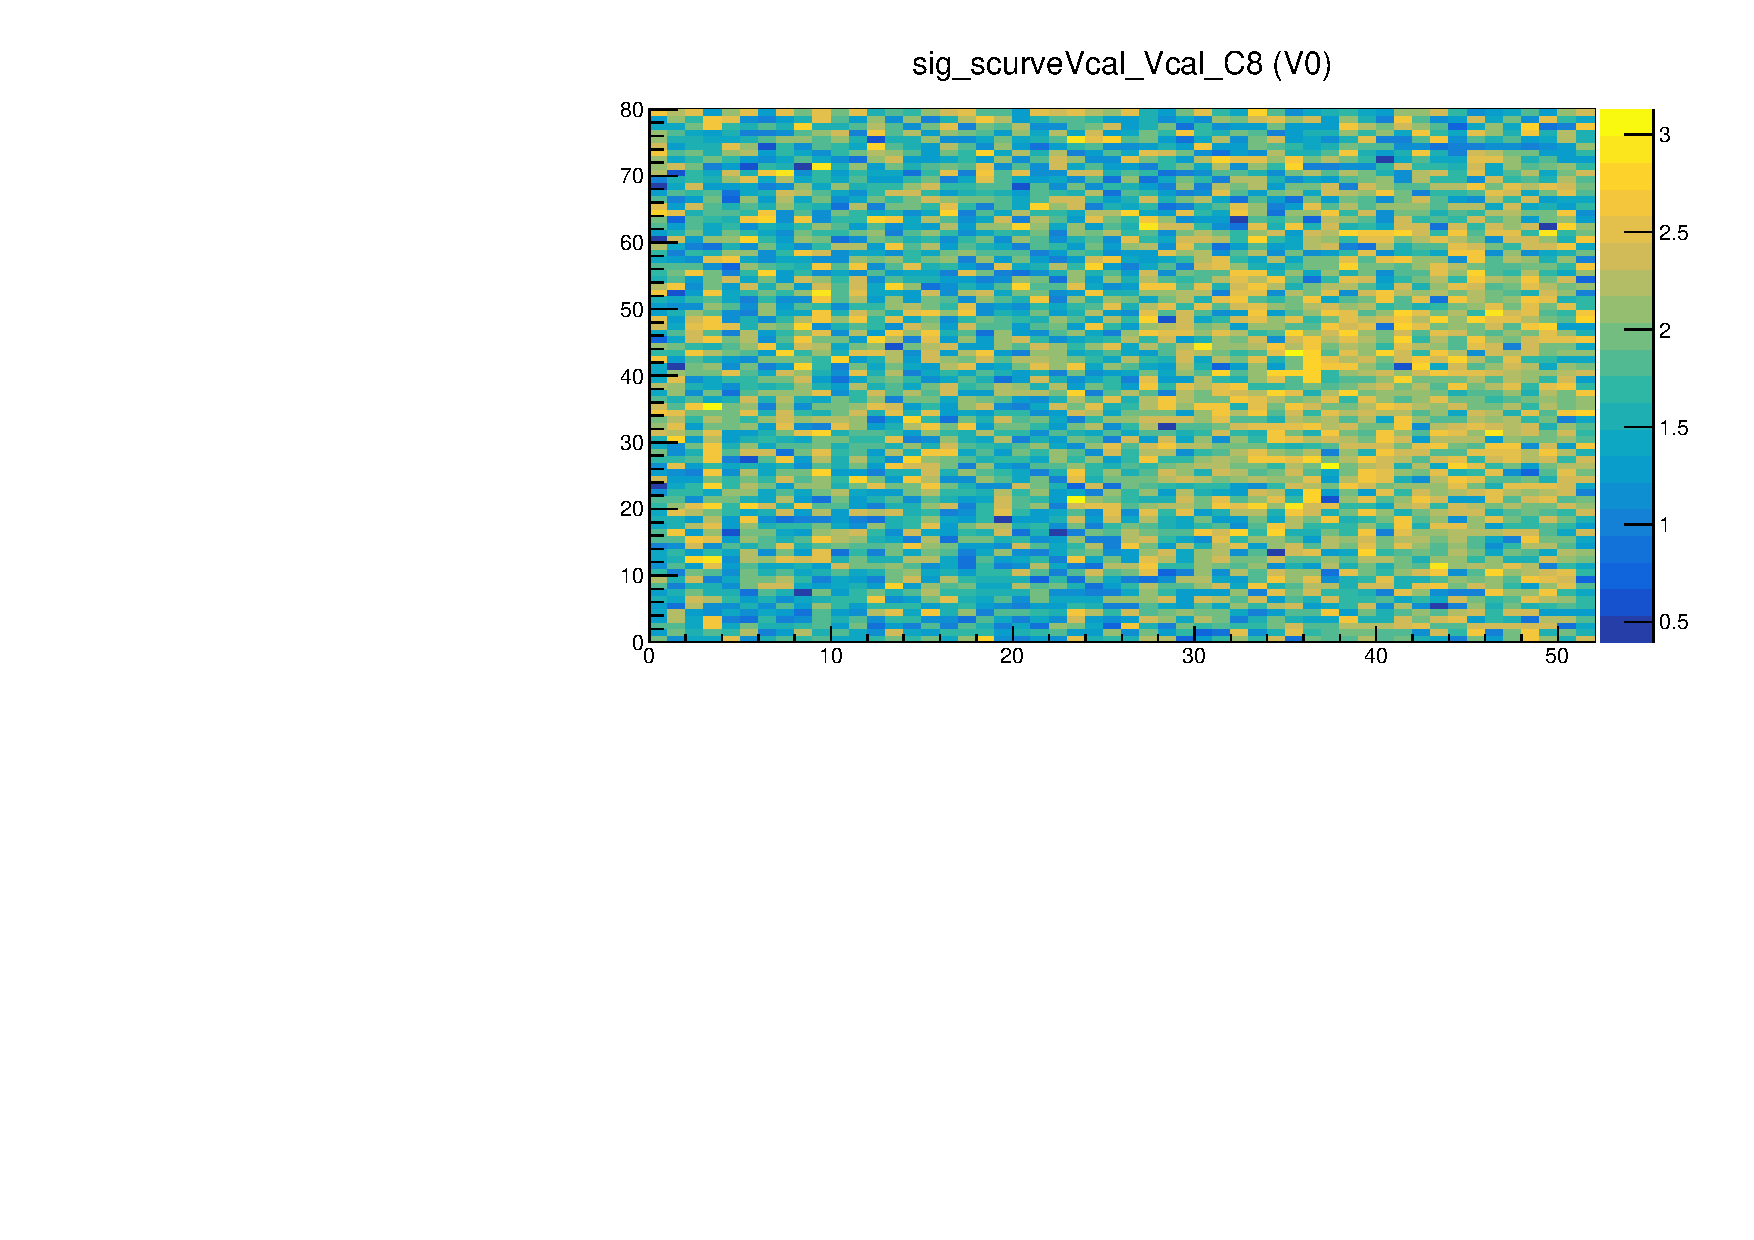
\includegraphics[width=0.5\textwidth]{ch7/scurve_map}
  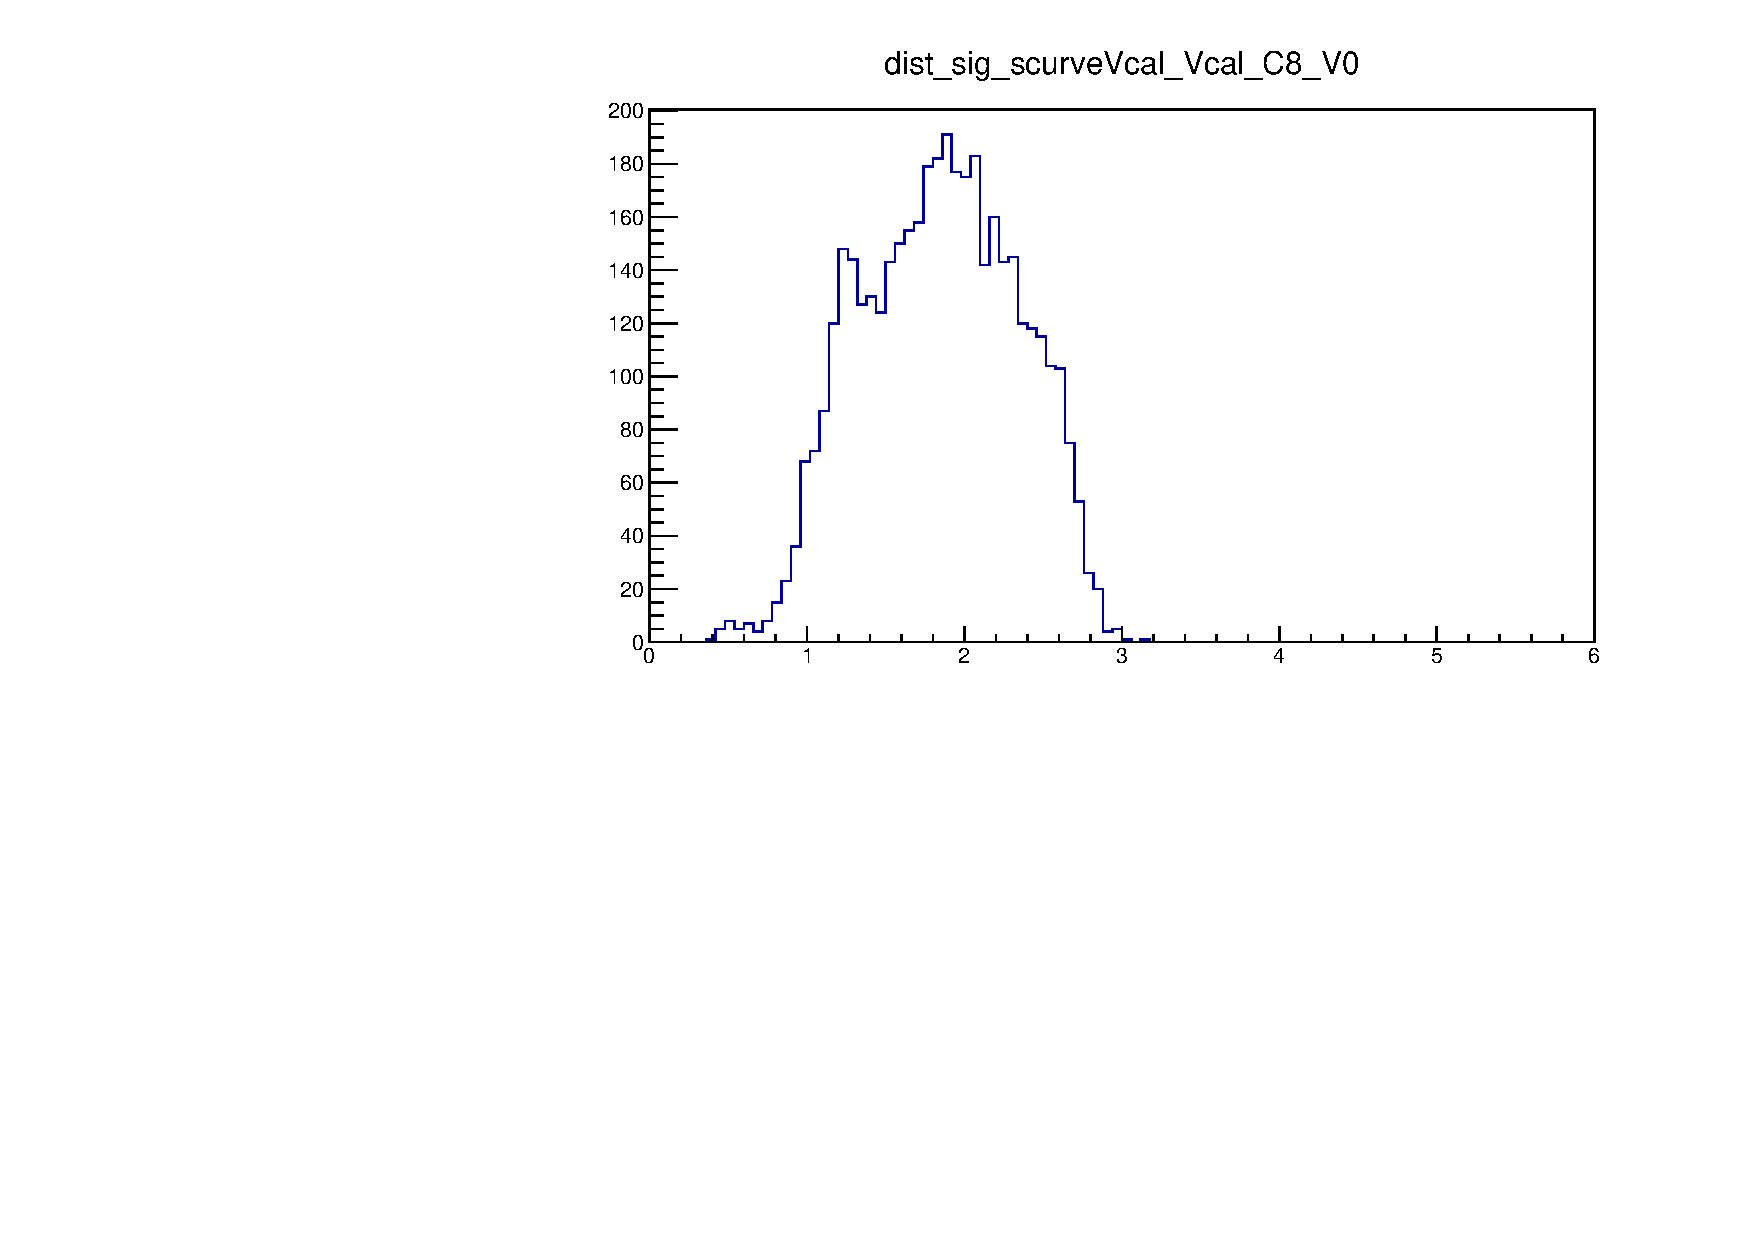
\includegraphics[width=0.5\textwidth]{ch7/scurve_dist}
  \caption[Scurve test]{Left: ROC map of the Vcal s-curve turn-on widths. Right: 1D distribution of the vcal scurve width.}\label{fig:vis_insp}
\end{figure}



\subsubsection{Bond Bonding Test}

%The BumpBonding test is meant to flag any problems with the bump bonds that connect the sensor to the ROCs and form the path for the charge generated in the silicon sensor to be recorded by the ROCs. This test takes advantage of a parallel route designed for the calibration signal in the ROC. This route can be seen at the top left of Figure 1, connecting the source of the Vcal calibration pulse to the “top metal pad” by closing the switch labeled “sensor calib” instead of the standard “calib” switch. The “top metal pad” is located near the edge of the ROC on the side facing the sensor. The calibration pulse can pass via capacitive coupling from this pad, across the ROC-sensor air gap, and into the silicon sensor. The calibration pulse then makes its way back into the ROC via the bump bond and can be read out as normal. Using this signal path that contains the bump bond, the presence of the bump and the quality of the electrical connection it establishes between the sensor and the ROC can be tested. Currently in pXar there are four variants of bump bonding tests, optimized to different module types. For FPix modules, the standard test is the BB3 test. This document focuses on this specific BumpBonding test version.


%The BumpBonding test is essentially an SCurve test with respect to VthrComp, with the calibration signal routed through the sensor instead of directly to the readout electronics. Vcal is configurable and by default is set to 250 (high range). In any case, Vcal should be set quite high since a large signal loss is expected going through the air gap from ROC to sensor. The number of triggers used is also configurable (default is 5). From the VthrComp s-curve for each pixel, the turn on value is extracted, defined as the value of VthrComp for which the efficiency surpasses 50%. For pixels with good bump bonds, these thresholds should be distributed normally, i.e. as a Gaussian curve. The distribution of the VthrComp turn-on is fitted to a Gaussian, the mean and width of which are recorded. In this fit, peaks near 0 or 255 are excluded, since these most likely come from dead pixels. Since variations in the mean of this turn-on are observed in odd and even columns, this fitting is done separately for the odd/even columns in the ROC. Pixels that turn on at much higher than average VthrComp values have higher than average signal loss. Leveraging this fact, pixels with turn-on values more than 5×σ above the mean are flagged as bad.





%The BumpBonding test is meant to flag any problems with the bump bonds that connect the sensor to the ROCs and form the path for the charge generated in the silicon sensor to be recorded by the ROCs. This test takes advantage of a parallel route designed for the calibration signal in the ROC. This route can be seen at the top left of Figure 1, connecting the source of the Vcal calibration pulse to the “top metal pad” by closing the switch labeled “sensor calib” instead of the standard “calib” switch. The “top metal pad” is located near the edge of the ROC on the side facing the sensor. The calibration pulse can pass via capacitive coupling from this pad, across the ROC-sensor air gap, and into the silicon sensor. The calibration pulse then makes its way back into the ROC via the bump bond and can be read out as normal. Using this signal path that contains the bump bond, the presence of the bump and the quality of the electrical connection it establishes between the sensor and the ROC can be tested. Currently in pXar there are four variants of bump bonding tests, optimized to different module types. For FPix modules, the standard test is the BB3 test. This document focuses on this specific BumpBonding test version.

%\begin{figure}[!h]
 % \centering
  %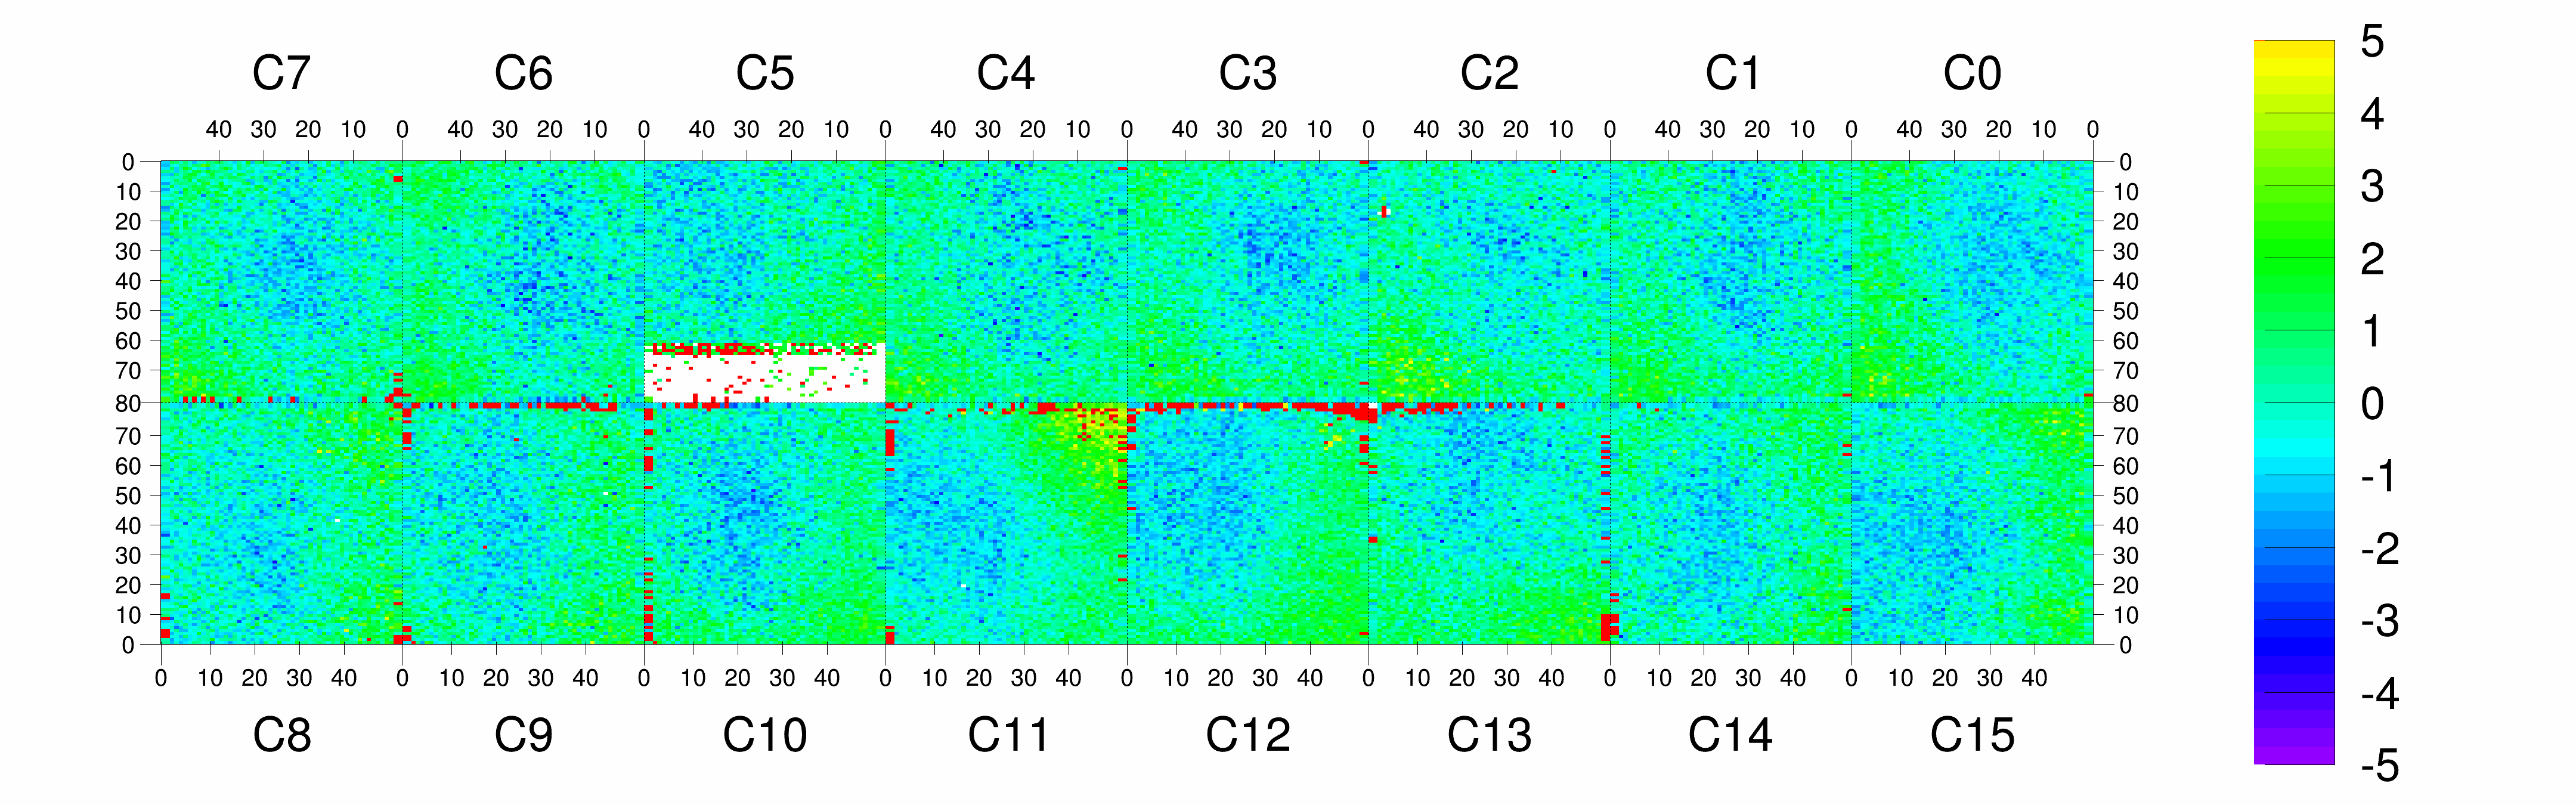
\includegraphics[width=0.7\textwidth]{ch7/bb_map}
  %\caption[Bond bonding test.]{Bond bonding test.}\label{fig:vis_insp}
%\end{figure}

\subsubsection{Summary}

%\begin{figure}[!h]
 % \centering
  %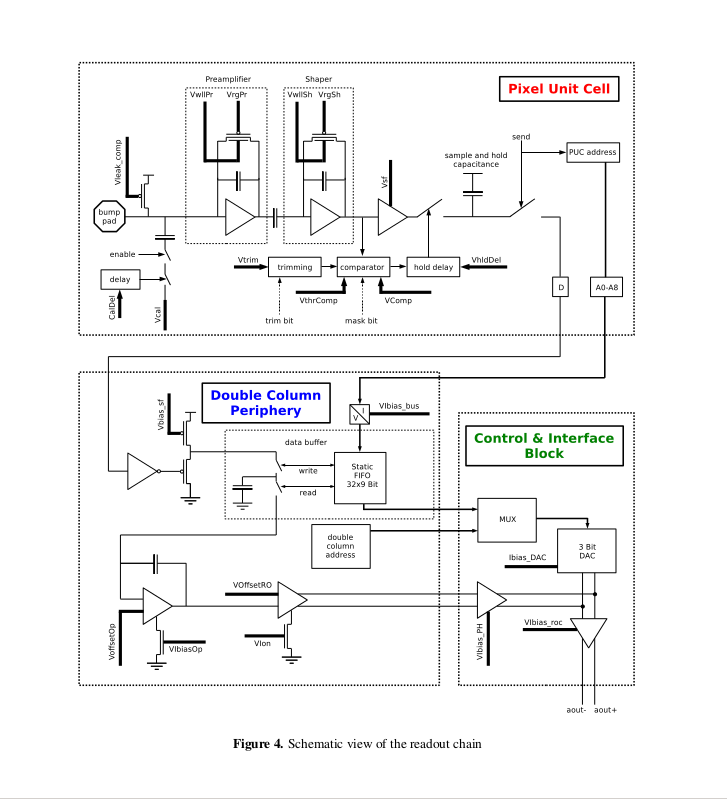
\includegraphics[width=0.7\textwidth]{../images/ch7/pix_unit_cell}
  %\caption[bla for index.]{bla bla.}\label{fig:pix_unit_cell}
%\end{figure}


%\begin{figure}[!h]
 % \centering
 % 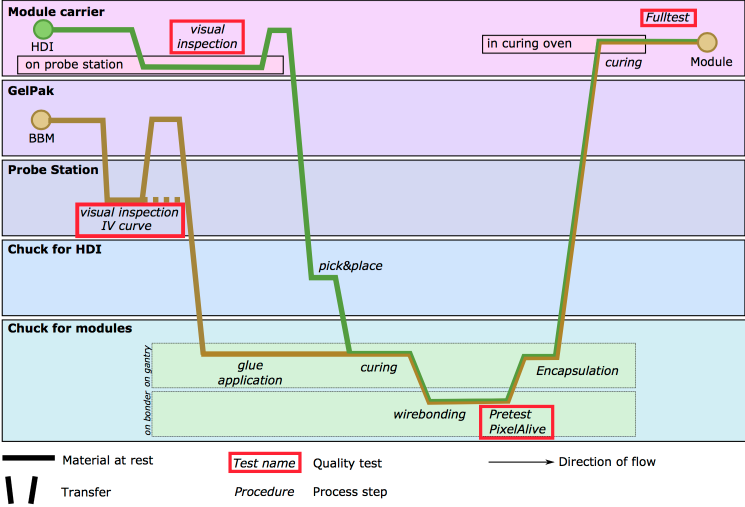
\includegraphics[width=0.7\textwidth]{../images/ch7/unl_workflow2}
 % \caption[bla for index.]{bla bla.}\label{fig:unl_workflow2}
%\end{figure}


%\begin{figure}[!h]
 % \centering
  %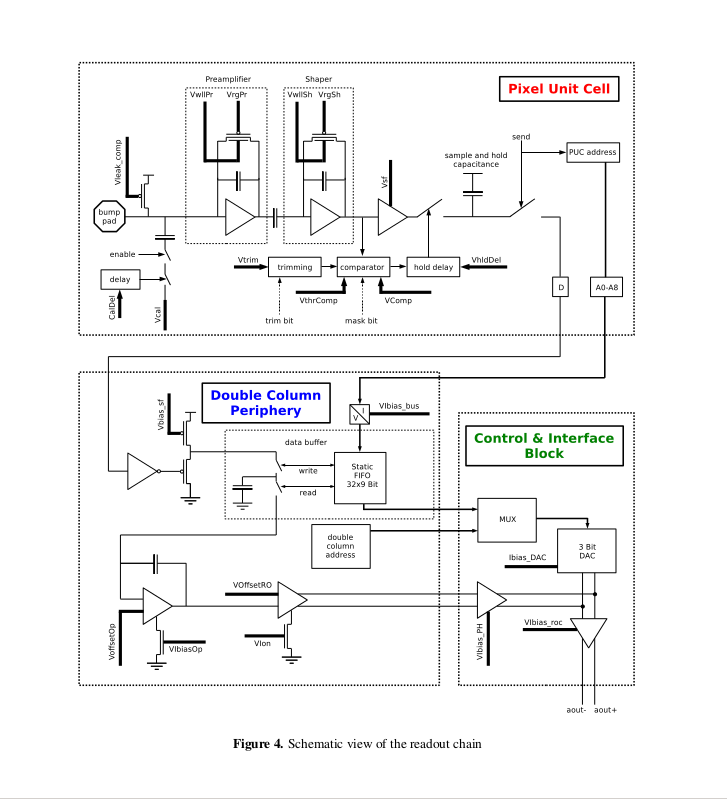
\includegraphics[width=0.7\textwidth]{../images/ch7/pix_unit_cell}
%  \caption[bla for index.]{bla bla.}\label{fig:pix_unit_cell}
%\end{figure}


%\begin{figure}[!h]
 % \centering
  %\includegraphics[width=0.7\textwidth]{../images/ch7/unl_workflow2}
%  \caption[bla for index.]{bla bla.}\label{fig:unl_workflow2}
%\end{figure}

%\begin{figure}[ht]
%\centering
%  \includegraphics[width=0.8\textwidth]{ch7/mod_ass_time}
 % \includegraphics[width=0.8\textwidth]{ch7/mod_ass_unl}
 %\caption[Module assembly over time.]{Module assembly over time for both assembly sites (top) and for UNL (bottom).}\label{fig:mod_ass_time}
%\end{figure}

%\begin{figure}[h]
%\begin{center}
 % \includegraphics[width=0.6\textwidth]{ch7/mod_grade_time}
  %\includegraphics[width=0.8\textwidth]{ch7/mod_grade_batch}
  %\caption[Module grade over time.]{Module grade over time (top) and per received batch at the integration site(bottom).}\label{fig:mod_grad_time}
%\end{center}
%\end{figure}

